\documentclass[cn,11pt,chinese,blue,bibstyle=ieeetr]{elegantbook}

\title{机器人学}
\subtitle{通向自由之路}

\author{Ray Roth}
\institute{Enabot}
\date{Jun 16, 2020}
\version{0.01}
%\bioinfo{自定义}{信息}

%\extrainfo{温柔正确的人总是难以生存,因为这世界既不温柔,也不正确。—— 比企谷八幡}

\logo{logo.png}
\cover{cover.jpg}


% 本文档命令
\usepackage{array}
\newcommand{\ccr}[1]{\makecell{{\color{#1}\rule{1cm}{1cm}}}}



\begin{document}

\maketitle
\frontmatter

\chapter*{自序}
\markboth{Introduction}{前言}
谨以记录我的逐梦之路,实践通向自由之路。

\vskip 1.5cm

\begin{flushright}
Ray Roth\\
Jun 16, 2020
\end{flushright}

\tableofcontents
%\listofchanges

\mainmatter


\chapter{运动学}

机械系统角度看,机械臂可用一组通过转动关节或移动关节连接的刚性连杆运动链抽象表示。该运动链的一端安装在基坐,末端执行器安装在运动链的另一端,将每个连杆相对前级连杆的基本运动进行合成即可得到运动链的整体运动情况。显然,为了在空间中操作目标,需要描述末端执行器位置和方向(简称位姿)。本章运用微积分和线性代数等高等数学基础知识,推导出正运动学方程,将末端执行器位姿表示为相对基坐标系机械结构(包括开链和闭链)中关节变量的函数。为最简化方向的表达,将引入操作空间概念,建立操作空间与关节空间的关系,进而对机械臂运动学参数进行标定。逆运动学问题即对给定的末端执行器位姿,计算满足末端执行器期望位姿要求的关节角。最后,将描述关节速度与末端执行器线速度与角速度之间的微分运动学关系,推导出雅可比矩阵。

\begin{introduction}
	\item \nameref{coordinate_system_and_pose_description}
	\item \nameref{transformation_of_coordinate_system}
	\item \nameref{direct_kinematics}
	\item \nameref{inverse_kinematics}
	\item \nameref{differential_kinematics_jacobi_matrix}
\end{introduction}


\section{坐标系和位姿描述}\label{coordinate_system_and_pose_description}

在描述物体间关系时,需要确定其所在坐标系的位置及方向,即通常所说的位姿。

\subsection{位姿描述}

\textbf{位置描述} 三维空间中任意一点可用位置矢量在直角坐标系${A}$中表示为:
\begin{equation}
^A\bm{p} = 
\begin{bmatrix}
p_x \\
p_y \\
p_z
\end{bmatrix}
\end{equation}
其中位置矢量 $^A\bm{p}$ 的上标 $A$ 表示参考坐标系 ${A}$,$\left(p_x, p_y, p_z\right)$ 表示点 $p$ 在坐标系 ${A}$ 坐标轴 $\left(\bm{x}_A, \bm{y}_A, \bm{z}_A\right)$ 上的三个分量。

\textbf{姿态描述或方向描述} 刚性物体的方向可由与其固定连接的坐标系描述。为描述空间中某物体 $B$ 的方向,设某直角坐标系 $\{B\}$ 与其固接,用坐标系 $\{B\}$ 的单位矢量 $\left(\bm{x}_B, \bm{y}_B, \bm{z}_B\right)$ 相对参考坐标系 ${A}$ 的方向余弦矩阵表示该刚体相对于参考坐标系的方向:
\begin{flalign}
_B^A\bm{R} = \begin{bmatrix}
_B^A\bm{x} & _B^A\bm{y} & _B^A\bm{z}
\end{bmatrix}
= \begin{bmatrix}
\bm{x}_B \cdot \bm{x}_A & \bm{y}_B \cdot \bm{x}_A & \bm{z}_B \cdot \bm{x}_A \\
\bm{x}_B \cdot \bm{y}_A & \bm{y}_B \cdot \bm{y}_A & \bm{z}_B \cdot \bm{y}_A \\
\bm{x}_B \cdot \bm{z}_A & \bm{y}_B \cdot \bm{z}_A & \bm{z}_B \cdot \bm{z}_A \\
\end{bmatrix}
\end{flalign}
其中 $_B^A\bm{R}$ 为正交单位矩阵,通常称为\textbf{旋转矩阵},式中上标 $A$ 表示参考坐标系,$B$表示被描述坐标系。旋转矩阵的列是被描述坐标系 ${B}$ 在参考坐标系 ${A}$ 中的描述,而其行是参考坐标系 ${A}$ 在被描述坐标系 ${B}$ 中的描述。

对应于参考坐标系坐标轴 $x$、$y$ 或 $z$ 轴旋转角度为 $\theta$ 的旋转矩阵分别为:
\begin{equation}\label{axis_x_rotation_matrix}
\bm{R}_x\left(\theta\right) = 
\begin{bmatrix}
1 & 0 		   & 0           \\
0 & \cos\theta & -\sin\theta \\
0 & \sin\theta & \cos\theta
\end{bmatrix}
\end{equation}

\begin{equation}\label{axis_y_rotation_matrix}
\bm{R}_y\left(\theta\right) = 
\begin{bmatrix}
\cos\theta  & 0 & \sin\theta \\
0           & 1 & 0          \\
-\sin\theta & 0 & \cos\theta
\end{bmatrix}
\end{equation}

\begin{equation}\label{axis_z_rotation_matrix}
\bm{R}_z\left(\theta\right) = 
\begin{bmatrix}
\cos\theta & -\sin\theta & 0 \\
\sin\theta & \cos\theta  & 0 \\
0          & 0           & 1
\end{bmatrix}
\end{equation}

\textbf{位姿描述} 完全描述刚体在空间中的位姿,通常将其与某坐标系 ${B}$ 固接,坐标原点一般选择刚体质心或其他特征点。那么相对参考坐标系 ${A}$,刚体固接坐标系 ${B}$ 的原点位置和坐标轴方向即可由位置向量 $^A\bm{p}_{B_o}$ 和旋转矩阵  $_B^A\bm{R}$ 描述,亦即刚体 $B$ 的位姿可由坐标系 ${B}$ 完全描述:
\begin{equation}
\left\lbrace B \right\rbrace = \left\lbrace _B^A\bm{R} \quad ^A\bm{p}_{B_o} \right\rbrace
\end{equation}


\subsection{常用姿态描述}

众所周知的旋转矩阵是种标准正交矩阵,其行列式为 $+1$。根据正交矩阵凯莱公式可知,对任何正交矩阵 $R$ 存在一个反对称矩阵 $S$,满足
\begin{equation}
\bm{R} = \left(\bm{I}-\bm{S}\right)^{-1} \cdot \left(\bm{I}+\bm{S}\right)
\end{equation}
因此,任何一个旋转矩阵可用三个参数确定。显然旋转矩阵的 $9$ 不是完全独立的,对每个旋转矩阵可写出 $6$ 个约束方程。假定 $R$ 为三列:
\begin{equation}
\bm{R}=\left(\bm{x} \quad \bm{y} \quad \bm{z}\right)
\end{equation}
这三个列矢量是坐标系的单位轴,每个列矢量都是单位向量,且相互垂直,即:
\begin{equation}
\begin{aligned}
|\bm{x}|=1 \\
|\bm{y}|=1 \\
|\bm{z}|=1 \\
\bm{x}\cdot\bm{y}=0 \\
\bm{x}\cdot\bm{z}=0 \\
\bm{y}\cdot\bm{z}=0
\end{aligned}
\end{equation}
由此可见,旋转矩阵可用三个参数简便表达,本节介绍几种常用姿态表示方法。


\subsubsection{\textbf{$RPY$}固定角}

每次旋转都是围绕参考坐标系的坐标轴旋转,这种姿态表示方法称作\textbf{固定角}。

\textbf{$RPY$角} 最终坐标系的方向\textbf{相对参考坐标系旋转}而来,可通过左乘基本旋转矩阵进行计算。即先绕参考坐标系的 $\bm{x}$ 轴旋转 $\gamma$,再绕参考坐标系的 $\bm{y}$ 轴旋转 $\beta$,最后绕参考坐标系的 $\bm{z}$ 轴旋转 $\alpha$:
\begin{equation}\label{rpy_fixed_angle}
	\begin{aligned}
		_B^A\bm{R}_{xyz}\left(\gamma, \beta, \alpha\right) &= \bm{R}_z\left(\alpha\right) \bm{R}_y\left(\beta\right) \bm{R}_x\left(\gamma\right) \\
		&=
		\begin{bmatrix}
			\cos\gamma & -\sin\gamma & 0 \\
			\sin\gamma & \cos\gamma  & 0 \\
			0          & 0           & 1
		\end{bmatrix}
		\begin{bmatrix}
			\cos\beta  & 0 & \sin\beta \\
			0           & 1 & 0          \\
			-\sin\beta & 0 & \cos\beta
		\end{bmatrix}
		\begin{bmatrix}
			1 & 0 		   & 0           \\
			0 & \cos\alpha & -\sin\alpha \\
			0 & \sin\alpha & \cos\alpha 
		\end{bmatrix} \\
		&=
		\begin{bmatrix}
			c\alpha c\beta & c\alpha s\beta s\gamma - s\alpha c\gamma & c\alpha s\beta c\gamma + s\alpha s\gamma \\
			s\alpha c\beta & s\alpha s\beta s\gamma + c\alpha c\gamma & s\alpha s\beta c\gamma - c\alpha s\gamma \\
			-s\beta        & c\beta s\gamma                           & c\beta c\gamma
		\end{bmatrix}
	\end{aligned}
\end{equation}

从上式可知,若已知旋转矩阵,则有 $9$ 个方程(其中 $6$ 个方程是相互关联的)和 $3$ 个未知量。令
\begin{equation}
	_B^A\bm{R}_{xyz}\left(\gamma, \beta, \alpha\right) =
	\begin{bmatrix}
		r_{11} & r_{12} & r_{13} \\
		r_{21} & r_{22} & r_{23} \\
		r_{31} & r_{32} & r_{33}
	\end{bmatrix}
\end{equation}
上式与式 \ref{rpy_fixed_angle} 对照,可求得:
\begin{equation}
	\begin{aligned}
		\beta &= -\arctan\frac{r_{31}}{\sqrt{r_{11}^2+r_{21}^2}} \\
		\alpha &= \arctan\frac{r_{21}/\cos\beta}{r_{11}/\cos\beta}, \quad (\cos\beta \ne 0) \\
		\gamma &= \arctan\frac{r_{32}/\cos\beta}{r_{33}/\cos\beta}, \quad (\cos\beta \ne 0)
	\end{aligned}
\end{equation}
若 $\beta = \pm 90^{\circ}$,即 $\cos\beta = 0$,此时仅能求出 $\alpha$ 和 $\beta$ 的和或差。这种情况下一般取 $\alpha = 0$,则有:
\begin{equation}
	\begin{aligned}
		\beta &= \pm 90^{\circ} \\
		\alpha &= 0 \\
		\gamma &= \pm \arctan\frac{r_{12}}{r_{22}}
	\end{aligned}
\end{equation}


\subsubsection{\textbf{$ZYX$}欧拉角}

\textbf{$ZYX$欧拉角} 最终坐标系的方向\textbf{相对当前坐标系旋转}而来,可通过右乘基本旋转矩阵进行计算。即先绕运动坐标系的 $\bm{z}$ 轴旋转 $\alpha$,再绕运动坐标系的 $\bm{y}$ 轴旋转 $\beta$,最后绕运动坐标系的 $\bm{x}$ 轴旋转 $\gamma$:
\begin{equation}
	_B^A\bm{R}_{zyx}\left(\alpha, \beta, \gamma\right) = \bm{R}_z\left(\alpha\right) \bm{R}_y\left(\beta\right) \bm{R}_x\left(\gamma\right)
\end{equation}
显然,三次绕固定轴旋转的最终姿态与以相反顺序绕运动轴旋转的最终姿态完全相同。


\subsubsection{\textbf{$ZYZ$}欧拉角}

每次旋转都是围绕运动坐标系的各轴旋转而不是绕参考坐标系固定轴旋转,这种姿态表示方法称作\textbf{欧拉角}。

\textbf{$ZYZ$欧拉角} 最终坐标系的方向\textbf{相对当前坐标系旋转}而来,可通过右乘基本旋转矩阵进行计算。即先绕运动坐标系的 $\bm{z}$ 轴旋转,再绕运动坐标系的 $\bm{y}$ 轴旋转,最后绕运动坐标系的 $\bm{z}$ 轴旋转:
\begin{equation}
	\begin{aligned}
		_B^A\bm{R}_{zyz}\left(\alpha, \beta, \gamma\right) &= \bm{R}_z\left(\alpha\right) \bm{R}_y\left(\beta\right) \bm{R}_z\left(\gamma\right) \\
		&=
		\begin{bmatrix}
			\cos\alpha & -\sin\alpha & 0 \\
			\sin\alpha & \cos\alpha  & 0 \\
			0          & 0           & 1
		\end{bmatrix}
		\begin{bmatrix}
			\cos\beta  & 0 & \sin\beta \\
			0           & 1 & 0          \\
			-\sin\beta & 0 & \cos\beta
		\end{bmatrix}
		\begin{bmatrix}
			\cos\gamma & -\sin\gamma & 0 \\
			\sin\gamma & \cos\gamma  & 0 \\
			0          & 0           & 1
		\end{bmatrix} \\
		&=
		\begin{bmatrix}
			c\alpha c\beta c\gamma - s\alpha s\gamma & -c\alpha c\beta s\gamma - s\alpha c\gamma & c\alpha s\beta \\
			s\alpha c\beta c\gamma + c\alpha s\gamma & -s\alpha c\beta s\gamma + c\alpha c\gamma & s\alpha s\beta \\
			-s\beta c\gamma                          & s\beta s\gamma                            & c\beta
		\end{bmatrix}
	\end{aligned}
\end{equation}

逆解可按前面的方法求得。当 $\sin\beta \ne 0$ 时:
\begin{equation}
	\begin{aligned}
		\beta &= \arctan\frac{\sqrt{r_{11}^2+r_{21}^2}}{r_{33}} \\
		\alpha &= \arctan\frac{r_{23}/\sin\beta}{r_{13}/\sin\beta}, \quad (\sin\beta \ne 0) \\
		\gamma &= -\arctan\frac{r_{32}/\sin\beta}{r_{31}/\sin\beta}, \quad (\sin\beta \ne 0)
	\end{aligned}
\end{equation}

当 $\beta=0$ 时:
\begin{equation}
	\begin{aligned}
		\beta &= 0 \\
		\alpha &= 0 \\
		\gamma &= \arctan\frac{-r_{12}}{r_{11}}
	\end{aligned}
\end{equation}

当 $\beta=180^{\circ}$ 时:
\begin{equation}
	\begin{aligned}
		\beta &= 180^{\circ} \\
		\alpha &= 0 \\
		\gamma &= \arctan\frac{r_{12}}{-r_{11}}
	\end{aligned}
\end{equation}


\section{坐标系变换}\label{transformation_of_coordinate_system}

对于任意一点 $p$ 在两个坐标系 ${A}$ 和 ${B}$ 中的描述 $^A\bm{p}$ 和 $^B\bm{p}$ 具有以下变换关系:
\begin{equation}\label{coordinate_system_transformation_equation}
^A\bm{p} = {^A\bm{p}}_{B_o} + {_B^A\bm{R}}^B\bm{p}
\end{equation}

\begin{figure}[htbp]
	\centering
	%set the plot display orientation
	%synatax: \tdplotsetdisplay{\theta_d}{\phi_d}
	\tdplotsetmaincoords{60}{110}
	
	%start tikz picture, and use the tdplot_main_coords style to implement the display 
	%coordinate transformation provided by 3dplot
	\begin{tikzpicture}[scale=5,tdplot_main_coords,
		point/.style={draw, circle, fill=black, inner sep=1pt},
		axisline/.style={thick,-{Triangle[width'=0pt .3, length=10pt]}},
		vecline/.style={thin,-{Triangle[width'=0pt .3, length=6pt]}},
		]
		
		%determine a coordinate (P) using (r,\theta,\phi) coordinates.  This command
		%also determines (Pxy), (Pxz), and (Pyz): the xy-, xz-, and yz-projections
		%of the point (P).
		%syntax: \tdplotsetcoord{Coordinate name without parentheses}{r}{\theta}{\phi}
		\tdplotsetcoord{O_A}{0}{0}{0}
		\tdplotsetcoord{O_B}{2}{45}{60}
		\tdplotsetcoord{O_C}{4}{38}{45}
		
		%set up some coordinates 
		%-----------------------
		\coordinate (A)  at (O_A) node[anchor=south east]{$O_A$};
		
		%draw the main coordinate system axes
		\draw[axisline] (0,0,0) -- (1,0,0) node[anchor=north east]{$\bm{x}_A$};
		\draw[axisline] (0,0,0) -- (0,1,0) node[anchor=north west]{$\bm{y}_A$};
		\draw[axisline] (0,0,0) -- (0,0,1) node[anchor=south]{$\bm{z}_A$} node[sloped,anchor=north west]{$\left\lbrace A \right\rbrace$};
		
		%set the rotated coordinate definition within display using a translation
		%coordinate and Euler angles in the "z(\alpha)y(\beta)z(\gamma)" euler rotation convention
		%syntax: \tdplotsetrotatedcoords{\alpha}{\beta}{\gamma}
		\tdplotsetrotatedcoords{45}{15}{30}
		
		%translate the rotated coordinate system
		%syntax: \tdplotsetrotatedcoordsorigin{point}
		\tdplotsetrotatedcoordsorigin{(O_B)}
		
		%use the tdplot_rotated_coords style to work in the rotated, translated coordinate frame
		\draw[tdplot_rotated_coords,axisline] (0,0,0) -- (1,0,0) node[anchor=north west]{$\bm{x}_B$};
		\draw[tdplot_rotated_coords,axisline] (0,0,0) -- (0,1,0) node[anchor=west]{$\bm{y}_B$};
		\draw[tdplot_rotated_coords,axisline] (0,0,0) -- (0,0,1) node[anchor=south]{$\bm{z}_B$} node[sloped,anchor=north west]{$\left\lbrace B \right\rbrace$};
		
		%draw vectors
		\draw[vecline] (O_A) -- node [sloped,above,pos=0.5] {$^A\bm{p}_{B_o}$} (O_B) node[anchor=south east]{$O_B$};
		
		\draw[vecline,tdplot_rotated_coords] (0,0,0) -- node [sloped,above,pos=0.5]{$^B\bm{p}$} (0.5,.25,.25) node[point, label={north east:$p$}]{};
		
		\draw[vecline,tdplot_rotated_coords] (O_A) -- node [sloped,below,pos=0.5]{$^A\bm{p}$} (0.5,.25,.25);
		
	\end{tikzpicture}
	\caption{坐标系变换}
\end{figure}

坐标系变换式 \ref{coordinate_system_transformation_equation} 对点 $^B\bm{p}$ 是非齐次的,可以用简洁的齐次变换形式表示为:
\begin{equation}\label{coordinate_system_homogeneous}
\begin{bmatrix}
^A\bm{p} \\
1
\end{bmatrix} = 
\begin{bmatrix}
_B^A\bm{R} & ^A\bm{p}_{B_o} \\
0 & 1
\end{bmatrix}
\begin{bmatrix}
^B\bm{p} \\
1
\end{bmatrix}
\end{equation}
式中 $4 \times 1$ 的\textbf{列向量称为点的齐次坐标},仍记作 $^A\bm{p}$ 和 $^B\bm{p}$,那么上式可表示为:
\begin{equation}
^A\bm{p} = {_B^A\bm{T}}{^B\bm{p}} = 
\begin{bmatrix}
{_B^A\bm{R}} & ^A\bm{p}_{B_o} \\
0 & 1
\end{bmatrix}
{^B\bm{p}}
\end{equation}

显然,齐次变换矩阵为:
\begin{equation}
{_B^A\bm{T}} = 
\begin{bmatrix}
{_B^A\bm{R}} & {^A\bm{p}_{B_o}} \\
0 & 1
\end{bmatrix}
\end{equation}

该矩阵的逆矩阵为:
\begin{equation}
{_B^A\bm{T}}^{-1} = 
{_A^B\bm{T}} = 
\begin{bmatrix}
{_A^B\bm{R}} & ^B\bm{p}_{A_o} \\
0 & 1
\end{bmatrix} = 
\begin{bmatrix}
{_B^A\bm{R}}^T & -{_B^A\bm{R}}^{T}{^A\bm{p}}_{B_o} \\
0 & 1
\end{bmatrix}
\end{equation}
其中,原点 $^A\bm{p}_{B_o}$ 在坐标系 $\left\{B\right\}$ 中描述为 $^B\left({^A\bm{p}}_{B_o}\right) = {_A^B\bm{R}}{^A\bm{p}}_{B_o} + {^B\bm{p}}_{A_o}$。坐标系原点在本坐标系描述为零,那么 $^B\left({^A\bm{p}}_{B_o}\right) = 0$,因此可得 $^B\bm{p}_{A_o} = -{_A^B\bm{R}}{^A\bm{p}}_{B_o} = -{_B^A\bm{R}}^{T}{^A\bm{p}}_{B_o}$。


\subsection{通用旋转变换}

通用旋转变换是指以任意矢量为轴进行旋转变换。

\subsubsection{通用旋转变换变换公式}

设 $\bm{f}$ 为坐标系 $\left\{C\right\}$ 的 $z$ 轴上的单位矢量,即
\begin{flalign}
\bm{C} &= \begin{bmatrix}
n_x & o_x & a_x & 0 \\
n_y & o_y & a_y & 0 \\
n_z & o_z & a_z & 0 \\
0   & 0   & 0   & 1
\end{bmatrix} \\
\bm{f} &= a_x\bm{i} + a_y\bm{j} + a_z\bm{k}
\end{flalign}
那么,绕矢量 $\bm{f}$ 旋转等价于绕坐标系 $\left\{C\right\}$ 的 $z$ 轴旋转,即
\begin{equation}
\bm{R}_f\left(\theta\right) = \bm{R}_{C_z}\left(\theta\right)
\end{equation}

若已知以参考坐标系描述的坐标系 $\left\{T\right\}$,那么可求得以坐标系 $\left\{C\right\}$ 描述的另一坐标系 $\left\{S\right\}$,因为
$$\bm{T} = \bm{C}\bm{S}$$
式中,$\bm{S}$ 表示 $\bm{T}$ 相对于 坐标系 $\left\{C\right\}$ 的位置。可求得
$$\bm{S}=\bm{C}^{-1}\bm{T}$$
显然,$\bm{T}$ 绕 $\bm{f}$ 旋转等价于 $\bm{S}$ 绕坐标系 $\left\{C\right\}$ 的 $z$ 轴旋转:
\begin{flalign}
\bm{R}_f\left(\theta\right)\bm{T} &= \bm{C}\bm{R}_z\left(\theta\right)\bm{S} =  \bm{C}\bm{R}_z\left(\theta\right)\bm{C}^{-1}\bm{T} \nonumber \\
\Longrightarrow \quad \bm{R}_f\left(\theta\right) &=  \bm{C}\bm{R}_z\left(\theta\right)\bm{C}^{-1} \nonumber \\
&= \begin{bmatrix}
n_x & o_x & a_x & 0 \\
n_y & o_y & a_y & 0 \\
n_z & o_z & a_z & 0 \\
0   & 0   & 0   & 1
\end{bmatrix}
\begin{bmatrix}
\cos\theta & -\sin\theta & 0 & 0 \\
\sin\theta & \cos\theta  & 0 & 0 \\
0          & 0           & 1 & 0 \\
0          & 0           & 0 & 1 \\
\end{bmatrix}
\begin{bmatrix}
n_x & n_y & n_z & 0 \\
o_x & o_y & o_z & 0 \\
a_x & a_y & a_z & 0 \\
0   & 0   & 0   & 1
\end{bmatrix} \nonumber \\ &=
\begin{array}{l}
\left[
\begin{array}{l}
n_xn_xc_{\theta} - n_xo_xs_{\theta} + n_xo_xs_{\theta} + o_xo_xc_{\theta} + a_xa_x \\
n_yn_xc_{\theta} - n_yo_xs_{\theta} + n_xo_ys_{\theta} + o_yo_xc_{\theta} + a_ya_x \\
n_zn_xc_{\theta} - n_zo_xs_{\theta} + n_xo_zs_{\theta} + o_zo_xc_{\theta} + a_za_x \\
0
\end{array} \right. \\ \left.
\begin{array}{l}
n_xn_yc_{\theta} - n_xo_ys_{\theta} + n_yo_xs_{\theta} + o_xo_yc_{\theta} + a_xa_y \\
n_yn_yc_{\theta} - n_yo_ys_{\theta} + n_yo_ys_{\theta} + o_yo_yc_{\theta} + a_ya_y \\
n_zn_yc_{\theta} - n_zo_ys_{\theta} + n_yo_zs_{\theta} + o_zo_yc_{\theta} + a_za_y \\
0
\end{array} \right. \\ \left.
\begin{array}{ll}
n_xn_zc_{\theta} - n_xo_zs_{\theta} + n_zo_xs_{\theta} + o_xo_zc_{\theta} + a_xa_y & 0 \\
n_yn_zc_{\theta} - n_yo_zs_{\theta} + n_zo_ys_{\theta} + o_yo_zc_{\theta} + a_ya_y & 0 \\
n_zn_zc_{\theta} - n_zo_zs_{\theta} + n_zo_zs_{\theta} + o_zo_zc_{\theta} + a_za_y & 0 \\
0 & 1
\end{array}
\right]
\end{array} \nonumber \\ &=
\begin{bmatrix}\label{general_rotation_transformation_equation}
f_xf_x \text{vers}\theta + c_{\theta}    & f_yf_x \text{vers}\theta - f_zs_{\theta} & f_zf_x \text{vers}\theta + f_ys_{\theta} & 0 \\
f_xf_y \text{vers}\theta + f_zs_{\theta} & f_yf_y \text{vers}\theta + c_{\theta}    & f_zf_y \text{vers}\theta - f_xs_{\theta} & 0 \\
f_xf_z \text{vers}\theta - f_ys_{\theta} & f_yf_z \text{vers}\theta + f_xs_{\theta} & f_zf_z \text{vers}\theta + c_{\theta}    & 0 \\
0                              & 0                              & 0                              & 1
\end{bmatrix}
\end{flalign}
其中,令 $f=z=a, \text{vers}\theta=1-c_{\theta}$,并根据正交矢量点积、矢量自乘、单位矢量和相似矩阵特征值等性质可化简推导出结论。


\subsubsection{等效转角与转轴}

给出任意旋转变换矩阵,即可由式 \ref{general_rotation_transformation_equation} 求得对应的转角和转轴。

已知旋转变换
\begin{equation}
\bm{R} = \begin{bmatrix}
n_x & o_x & a_x & 0 \\
n_y & o_y & a_y & 0 \\
n_z & o_z & a_z & 0 \\
0   & 0   & 0   & 1
\end{bmatrix} \nonumber
\end{equation}
令 $\bm{R} = \bm{R}_f\left(\theta\right)$,即
\begin{flalign}
&\begin{bmatrix}
n_x & o_x & a_x & 0 \\
n_y & o_y & a_y & 0 \\
n_z & o_z & a_z & 0 \\
0   & 0   & 0   & 1
\end{bmatrix} \nonumber \\
= &\begin{bmatrix}
f_xf_x \text{vers}\theta + c_{\theta}    & f_yf_x \text{vers}\theta - f_zs_{\theta} & f_zf_x \text{vers}\theta + f_ys_{\theta} & 0 \\
f_xf_y \text{vers}\theta + f_zs_{\theta} & f_yf_y \text{vers}\theta + c_{\theta}    & f_zf_y \text{vers}\theta - f_xs_{\theta} & 0 \\
f_xf_z \text{vers}\theta - f_ys_{\theta} & f_yf_z \text{vers}\theta + f_xs_{\theta} & f_zf_z \text{vers}\theta + c_{\theta}    & 0 \\
0                              & 0                              & 0                              & 1
\end{bmatrix}
\end{flalign}
将等式两边按对角项分别相加,以及非对角项成对相减,并化简得
\begin{flalign}
n_x + o_y + a_z &= \left(f_x^2 + f_y^2 + f_z^2\right) vers\theta + 3c_{\theta} = 1 + 2c_{\theta} \nonumber \\
\Longrightarrow c_{\theta} &= \frac{1}{2}\left(n_x + o_y + a_z - 1\right) \\ \nonumber \\
2f_xs_{\theta} &= o_z - a_y \nonumber \\
2f_ys_{\theta} &= a_x - n_z \nonumber \\
2f_zs_{\theta} &= n_y - o_x \nonumber \\
\Longrightarrow 4s^2\theta &= \left(o_z - a_y\right)^2 + \left(a_x - n_z\right)^2 + \left(n_y - o_x\right)^2 \nonumber \\
\Longrightarrow s_{\theta} &= \pm \frac{1}{2} \sqrt{\left(o_z - a_y\right)^2 + \left(a_x - n_z\right)^2 + \left(n_y - o_x\right)^2}
\end{flalign}
规定旋转为绕转轴矢量 $\bm{f}$ 的正向旋转,即 $0 \le \theta \le 180^{\circ}$,此时 $\sin\theta$ 取正号,那么转角 $\theta$ 可被唯一确定为:
\begin{equation}
\tan\theta = \frac{\sqrt{\left(o_z - a_y\right)^2 + \left(a_x - n_z\right)^2 + \left(n_y - o_x\right)^2}}{n_x + o_y + a_z - 1}
\end{equation}
且转轴矢量 $\bm{f}$ 的各分量为:
\begin{equation}
\left\{\begin{array}{c}
f_x = \frac{o_z - a_y}{2s_{\theta}} \\
f_y = \frac{a_x - n_z}{2s_{\theta}} \\
f_z = \frac{n_y - o_x}{2s_{\theta}}
\end{array}
\right.
\end{equation}


\subsubsection{单位四元数}

未完待续 \\
未完待续 \\
未完待续 \\
未完待续 \\
未完待续 \\
未完待续 \\


\subsection{变换方程}

坐标系 $\left\{D\right\}$ 可以用两种不同的方式变换到坐标系 $\left\{U\right\}$。

第一种方式:
$${_D^UT}={_A^UT}{_D^AT}$$

第二种方式:
$${_D^UT}={_B^UT}{_C^BT}{_D^CT}$$
将上述两个表达式构造成变换方程:
\begin{equation}\label{transformation_equation}
{_A^UT}{_D^AT}={_B^UT}{_C^BT}{_D^CT}
\end{equation}

若有 $n$ 个未知变换和 $n$ 个变换方程,那么所有变换可有变换方程组解出。式 \ref{transformation_equation} 中除 $T_C^B$ 外所有变换均已知,一个变换方程一个未知变换,容易解出:
\begin{equation}
_C^BT={_B^UT}^{-1}{ _A^UT}{_D^AT} {_D^CT}^{-1}
\end{equation}

\begin{figure}[htbp]
	\centering
	%set the plot display orientation
	%synatax: \tdplotsetdisplay{\theta_d}{\phi_d}
	\tdplotsetmaincoords{60}{110}
	
	%start tikz picture, and use the tdplot_main_coords style to implement the display 
	%coordinate transformation provided by 3dplot
	\begin{tikzpicture}[scale=3,tdplot_main_coords,
		point/.style={draw, circle, fill=black, inner sep=1pt},
		axisline/.style={thick,-{Triangle[width'=0pt .3, length=10pt]}},
		vecline/.style={thin,-{Triangle[width'=0pt .3, length=6pt]}},
		]
		
		%determine a coordinate (P) using (r,\theta,\phi) coordinates.  This command
		%also determines (Pxy), (Pxz), and (Pyz): the xy-, xz-, and yz-projections
		%of the point (P).
		%syntax: \tdplotsetcoord{Coordinate name without parentheses}{r}{\theta}{\phi}
		\tdplotsetcoord{O_U}{0}{0}{0}
		\tdplotsetcoord{O_A}{1.8}{15}{60}
		\tdplotsetcoord{O_B}{4}{62}{46}
		\tdplotsetcoord{O_C}{6.5}{55}{55}
		\tdplotsetcoord{O_D}{4.5}{40}{60}
		
		%set up some coordinates 
		%-----------------------
		\coordinate (U)  at (O_U) node[anchor=south east]{$O_U$};
		
		%draw the main coordinate system axes
		\draw[axisline] (0,0,0) -- (1,0,0) node[anchor=north east]{$\bm{x}_U$};
		\draw[axisline] (0,0,0) -- (0,1,0) node[anchor=north west]{$\bm{y}_U$};
		\draw[axisline] (0,0,0) -- (0,0,1) node[anchor=south]{$\bm{z}_U$} node[sloped,anchor=north east]{$\left\lbrace U \right\rbrace$};
		
		%set the rotated coordinate definition within display using a translation
		%coordinate and Euler angles in the "z(\alpha)y(\beta)z(\gamma)" euler rotation convention
		%syntax: \tdplotsetrotatedcoords{\alpha}{\beta}{\gamma}
		\tdplotsetrotatedcoords{15}{-15}{45}
		
		%translate the rotated coordinate system
		%syntax: \tdplotsetrotatedcoordsorigin{point}
		\tdplotsetrotatedcoordsorigin{(O_A)}
		
		%use the tdplot_rotated_coords style to work in the rotated, translated coordinate frame
		\draw[tdplot_rotated_coords,axisline] (0,0,0) -- (1,0,0) node[anchor=north west]{$\bm{x}_A$};
		\draw[tdplot_rotated_coords,axisline] (0,0,0) -- (0,1,0) node[anchor=west]{$\bm{y}_A$};
		\draw[tdplot_rotated_coords,axisline] (0,0,0) -- (0,0,1) node[anchor=south]{$\bm{z}_A$} node[sloped,anchor=north west]{$\left\lbrace A \right\rbrace$};
		
		%set the rotated coordinate definition within display using a translation
		%coordinate and Euler angles in the "z(\alpha)y(\beta)z(\gamma)" euler rotation convention
		%syntax: \tdplotsetrotatedcoords{\alpha}{\beta}{\gamma}
		\tdplotsetrotatedcoords{45}{-15}{30}
		
		%translate the rotated coordinate system
		%syntax: \tdplotsetrotatedcoordsorigin{point}
		\tdplotsetrotatedcoordsorigin{(O_B)}
		
		%use the tdplot_rotated_coords style to work in the rotated, translated coordinate frame
		\draw[tdplot_rotated_coords,axisline] (0,0,0) -- (1,0,0) node[anchor=north west]{$\bm{x}_B$};
		\draw[tdplot_rotated_coords,axisline] (0,0,0) -- (0,1,0) node[anchor=west]{$\bm{y}_B$};
		\draw[tdplot_rotated_coords,axisline] (0,0,0) -- (0,0,1) node[anchor=south]{$\bm{z}_B$} node[sloped,anchor=north west]{$\left\lbrace B \right\rbrace$};
		
		%set the rotated coordinate definition within display using a translation
		%coordinate and Euler angles in the "z(\alpha)y(\beta)z(\gamma)" euler rotation convention
		%syntax: \tdplotsetrotatedcoords{\alpha}{\beta}{\gamma}
		\tdplotsetrotatedcoords{-30}{-30}{15}
		
		%translate the rotated coordinate system
		%syntax: \tdplotsetrotatedcoordsorigin{point}
		\tdplotsetrotatedcoordsorigin{(O_C)}
		
		%use the tdplot_rotated_coords style to work in the rotated, translated coordinate frame
		\draw[tdplot_rotated_coords,axisline] (0,0,0) -- (1,0,0) node[anchor=north west]{$\bm{x}_C$};
		\draw[tdplot_rotated_coords,axisline] (0,0,0) -- (0,1,0) node[anchor=west]{$\bm{y}_C$};
		\draw[tdplot_rotated_coords,axisline] (0,0,0) -- (0,0,1) node[anchor=south]{$\bm{z}_C$} node[sloped,anchor=north west]{$\left\lbrace C \right\rbrace$};
		
		%set the rotated coordinate definition within display using a translation
		%coordinate and Euler angles in the "z(\alpha)y(\beta)z(\gamma)" euler rotation convention
		%syntax: \tdplotsetrotatedcoords{\alpha}{\beta}{\gamma}
		\tdplotsetrotatedcoords{30}{-45}{15}
		
		%translate the rotated coordinate system
		%syntax: \tdplotsetrotatedcoordsorigin{point}
		\tdplotsetrotatedcoordsorigin{(O_D)}
		
		%use the tdplot_rotated_coords style to work in the rotated, translated coordinate frame
		\draw[tdplot_rotated_coords,axisline] (0,0,0) -- (1,0,0) node[anchor=north west]{$\bm{x}_D$};
		\draw[tdplot_rotated_coords,axisline] (0,0,0) -- (0,1,0) node[anchor=west]{$\bm{y}_D$};
		\draw[tdplot_rotated_coords,axisline] (0,0,0) -- (0,0,1) node[anchor=south]{$\bm{z}_D$} node[sloped,anchor=north west]{$\left\lbrace D \right\rbrace$};
		
		%draw vectors
		\draw[vecline] (O_U) -- node [sloped,below,pos=0.5] {$^U\bm{p}_{A_o}$} (O_A) node[anchor=south east]{$O_A$};
		\draw[vecline] (O_A) -- node [sloped,above,pos=0.5] {$^A\bm{p}_{D_o}$} (O_D) node[anchor=south east]{$O_D$};
		\draw[vecline] (O_U) -- node [sloped,above,pos=0.5] {$^U\bm{p}_{B_o}$} (O_B) node[anchor=south east]{$O_B$};
		\draw[vecline] (O_B) -- node [sloped,below,pos=0.5] {$^B\bm{p}_{C_o}$} (O_C) node[anchor=south west, rotate=-15]{$O_C$};
		\draw[vecline] (O_C) -- node [sloped,above,pos=0.5] {$^C\bm{p}_{D_o}$} (O_D) node[anchor=south east]{$O_D$};
	\end{tikzpicture}
	\caption{闭环变换形成的变换组}
\end{figure}

上图采用了\textbf{坐标系的图形表示法},用从上一个坐标系的原点指向下一个坐标系的原点的箭头定义坐标系,箭头的指向指明了坐标系定义方式,即下一个坐标系相对于上一个坐标系定义,将箭头串联起来,通过简单的变换相乘即可得到复合坐标系。若某个箭头的方向与串联箭头的方向相反,首先求出其逆,然后按串联次序相乘即可。


\subsection{数值计算}


\section{正运动学}\label{direct_kinematics}

运动学研究机械系统的运动特性,但不考虑使其产生运动的力,主要研究对象是系统的位置、速度、加速度,以及位置变量对时间和其他变量的高阶导数。机械臂由一系列连杆(刚体)通过关节(运动副)连接起来,关节可分为两大类:转动型和移动型,机械臂整个结构型成一个运动链,一端固定在基座上,另一端连接末端执行器。运动链两端只由一系列连杆相连接的成为开链,若连杆形成了闭环则称为闭链。机械臂结构及姿态由自由度表征,典型情况下每个自由度与一个关节关联,亦即关节变量,正运动学研究核心是根据关节变量计算末端执行器的姿态。

一般情况下,刚体相对参考坐标系的位姿由原点的位置向量和固连在刚体的坐标系的单位向量描述。相对参考坐标系 $O_b-x_by_bz_b$,正运动学方程可表示为:
\begin{equation}
{_e^b\bm{T}}\left(\bm{q}\right) = \begin{bmatrix}
{_e^b\bm{n}}\left(\bm{q}\right) & {_e^b\bm{o}}\left(\bm{q}\right) & {_e^b\bm{a}}\left(\bm{q}\right) & {_e^b\bm{p}}\left(\bm{q}\right)
\end{bmatrix}
\end{equation}
其中 $\bm{q}$ 为关节变量,$\left(\bm{n}_e,\bm{o}_e,\bm{a}_e\right)$ 为固连在末端执行器坐标系的单位向量,$\bm{p}_e$ 为该坐标系原点相对基坐标系原点的位置向量。坐标系 $O_b-x_by_bz_b$ 定义为基坐标系,固连在末端执行器的坐标系定义为末端执行器坐标系,通常根据任务特性所使用的末端执行器选择。若末端执行器为单自由度钳形工具,那么末端执行器的坐标系原点就定位在该工具中心,单位向量 $\bm{a}_e$ 选为接近目标的方向,单位向量 $\bm{o}_e$ 在钳口滑动平面内且垂直于 $\bm{a}_e$,单位向量 $\bm{n}_e$ 与另外两个单位向量垂直且使坐标系 $O_b-x_by_bz_b$ 符合右手法则。

正运动学的第一种计算方式是通过对机械结构的几何分析进行,但是该方法的有效性取决于选取适当的系统变量,以及研究者几何分析能力,当系统较为复杂、关节数量较多时就不太适用了。


\subsection{开链系统}

典型的开链机械臂通过 $n$ 个关节连接 $n+1$ 个连杆构成,假设其连杆 $0$ 固定在地面,且每个关节为机械结构提供一个与关节变量对应的自由度。由于每个关节连接相邻的两个连杆,通常首先分析相邻连杆的运动学关系描述,然后通过递归方式计算整个开链系统的运动学描述。为每个连杆顺序定义固连坐标系,那么坐标系 $n$ 的位姿相对于坐标系 $0$ 的坐标变换可由下式给出:
\begin{equation}\label{link_forward_coordinate_transformation}
{_n^0\bm{T}}\left(\bm{q}\right) = {_1^0\bm{T}}\left(q_1\right){_2^1\bm{T}}\left(q_2\right)\cdots{_n^{n-1}\bm{T}}\left(q_n\right)
\end{equation}
其中,每个齐次变换矩阵都是相应关节变量的函数,可采用递归与齐次变换矩阵乘积计算得出正运动学方程。

描述末端执行器坐标系相对于基坐标系位姿的坐标变换可表示为:
\begin{equation}
{_e^b\bm{T}\left(\bm{q}\right)} = {_0^b\bm{T}}{_n^0\bm{T}\left(\bm{q}\right)}{_e^n\bm{T}}
\end{equation}
其中 $_0^b\bm{T}$ 和 $_e^n\bm{T}$ 为常数变换矩阵,分别用于描述坐标系 $0$ 相对于基坐标系的位姿,以及末端执行器坐标系相对于坐标系 $n$ 的位姿。


\subsection{标准Denavit-Hartenberg方法}

为系统化的描述可使用递归形式计算的开链机械臂正运动学方程,引入了 DH 方法,该方法通过标准 DH 模型(简写为SDH,Standard Denavit-Hartenberg)定义连杆坐标系(见图 \ref{sdh_model_description}),定义规则如下:

\begin{enumerate}
\item $z_i$ 轴选择为关节 $i+1$ 的轴方向;
\item 原点$O_i$ 选择为 $z_{i+1}$ 轴与 $z_i$ 轴的公垂线与 $z_i$ 轴的交点;
\item $x_i$ 轴选择为 $z_{i+1}$ 轴与 $z_i$ 轴的公垂线,方向由关节 $i$ 指向关节 $i+1$;
\item $y_i$ 轴根据右手系规则确定。
\end{enumerate}

\begin{figure}[htbp]
	\centering
	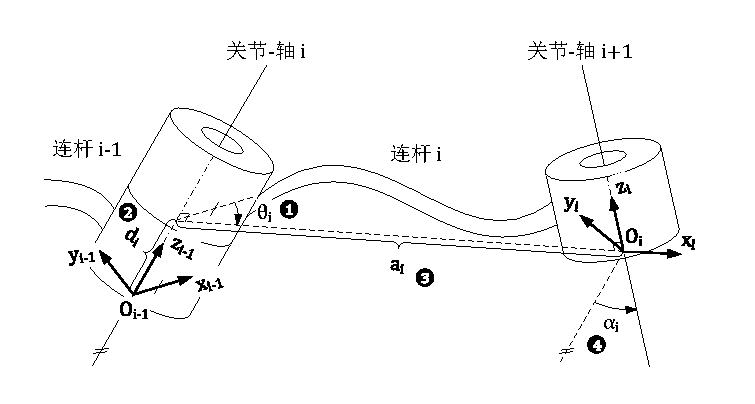
\includegraphics[scale=1]{images//sdh_model.pdf} \\
	\caption{SDH模型描述图}
	\label{sdh_model_description}
\end{figure}

特殊情况下 DH 模型的关节坐标系定义不唯一:
\begin{enumerate}
\item 基坐标系 $\left\{0\right\}$ 只有 $z_0$ 方向是指定的,$O_0$ 和 $x_0$ 可以任意选择。当第一个关节变量为零时,一般规定坐标系 $\left\{0\right\}$ 和 $\left\{1\right\}$ 重合;
\item 末端坐标系 $\left\{n\right\}$ 没有关节 $n+1$,$z_n$ 不是唯一定义的,其原点和 $x_n$ 随 $z_n$ 可任意选取(其 $x_n$ 和 $z_{n-1}$ 仍然必须垂直)。例如,在选取时尽量使连杆参数为零。或者,若关节 $n$ 是转动型的,那么 $z_n$ 将参考 $z_{n-1}$ 的方向设置;
\item 当相邻两个关节轴平行时(连杆扭角$\alpha=0$),公垂线不唯一;
\item 当相邻两个关节轴相交时(连杆长度$a=0$),$x_i$ 方向是任意的;
\item 当关节 $i$ 为移动型时,$z_{i-1}$ 方向是任意的。
\end{enumerate}
可以根据这些不明确的特性来简化坐标系定义。例如,相邻坐标系的轴可选为平行的、垂直的或者使 $d=0$ 等等。

连杆坐标系定义完成后,坐标系 $i$ 相对于坐标系 $i-1$ 的位姿即完全由以下参数确定:
\begin{enumerate}
\item 连杆夹角 $\theta_{i}$ :$x_{i-1}$ 轴与 $x_i$ 轴绕 $z_{i-1}$ 轴的夹角;
\item 连杆偏移 $d_{i}$ :$x_{i-1}$ 沿 $z_{i-1}$ 轴到 $x_i$ 轴的距离;
\item 关节扭角 $\alpha_{i}$ :$z_{i-1}$ 轴与 $z_i$ 轴绕 $x_{i-1}$ 轴的夹角;
\item 连杆长度 $a_{i}$ :$z_{i-1}$ 轴沿 $x_i$ 轴到 $z_i$ 轴的距离;
\item 关节类型 $\sigma_i$ :对于转动关节,广义关节变量 $q_i$ 变为 $\theta_{i}$;对于移动关节,广义关节变量 $q_i$ 变为 $d_i$。
\end{enumerate}

上述参数中连杆扭角、连杆长度即连杆类型均为定值,对于每个连杆只有一个参数是变量,由此,坐标系 $\left\{i\right\}$ 相对于坐标系 $\left\{i-1\right\}$ 坐标变换可按如下变换顺序,逐次右乘单个变换得到,即:
\begin{equation}\label{sdh_model_adjacent_link_forward_coordinate_transformation}
	\begin{aligned}
		{_i^{i-1}\bm{T}} &= \bm{R}_z\left(\theta_i\right)\bm{T}_z\left(d_i\right)\bm{T}_x\left(a_i\right)\bm{R}_x\left(\alpha_i\right) \\
		&= 
		\begin{bmatrix}
			c_{\theta_i} & -s_{\theta_i} & 0 & 0 \\
			s_{\theta_i} & c_{\theta_i}  & 0 & 0 \\
			0         & 0          & 1 & 0 \\
			0         & 0          & 0 & 1
		\end{bmatrix}
		\begin{bmatrix}
			1 & 0 & 0 & 0   \\
			0 & 1 & 0 & 0   \\
			0 & 0 & 1 & d_i \\
			0 & 0 & 0 & 1
		\end{bmatrix}
		\begin{bmatrix}
			1 & 0 & 0 & a_i \\
			0 & 1 & 0 & 0   \\
			0 & 0 & 1 & 0   \\
			0 & 0 & 0 & 1
		\end{bmatrix}
		\begin{bmatrix}
			1 & 0 		  & 0          & 0 \\
			0 & c_{\alpha_i} & -s_{\alpha_i} & 0 \\
			0 & s_{\alpha_i} & c_{\alpha_i}  & 0 \\
			0 & 0         & 0          & 1
		\end{bmatrix} \\
		&= \begin{bmatrix}
			c_{\theta_i} & -s_{\theta_i} c_{\alpha_i} & s_{\theta_i} s_{\alpha_i}  & a_i c_{\theta_i} \\
			s_{\theta_i} & c_{\theta_i} c_{\alpha_i}  & -c_{\theta_i} s_{\alpha_i} & a_i s_{\theta_i} \\
			0         & s_{\alpha_i}            & c_{\alpha_i}            & d_i           \\
			0         & 0                    & 0                    & 1
		\end{bmatrix}
	\end{aligned}
\end{equation}
该变换矩阵是广义关节坐标 $q_i$ 的函数,若是转动关节则该变量为 $\theta_i$,若是移动关节则该变量为 $d_i$。

\subsection{修正Denavit-Hartenberg方法}

DH 方法的另外一种形式是使用 MDH(Modified Denavit-Hartenberg)模型定义连杆坐标系。MDH 与 SDH 的最大区别是将连杆坐标系定义到相对基坐标系的近端,而不是远端(见图 \ref{mdh_model_description}),此外 SDH 坐标系在处理树形结构时会产生歧义,而 MDH 坐标系则不会发生这种情况。

\begin{figure}[htbp]
	\centering
	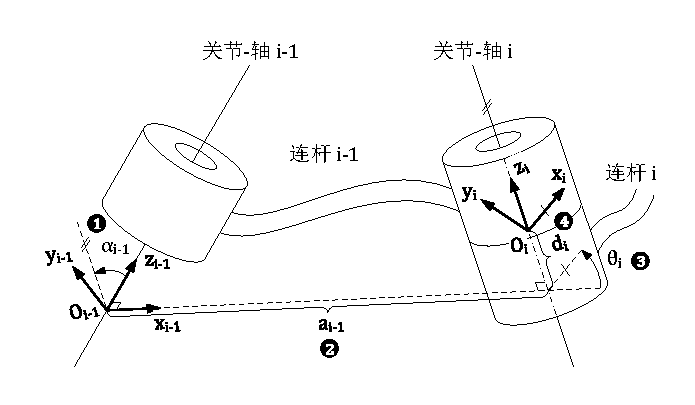
\includegraphics[scale=1]{images//mdh_model.pdf} \\
	\caption{MDH模型描述图}
	\label{mdh_model_description}
\end{figure}

MDH 连杆坐标系定义完成后,坐标系 $i$ 相对于坐标系 $i-1$ 的位姿即完全由以下参数确定:
\begin{enumerate}
	\item 关节扭角 $\alpha_{i-1}$ :$z_{i-1}$ 轴与 $z_i$ 轴绕 $x_{i-1}$ 轴的夹角;
	\item 连杆长度 $a_{i-1}$ :$z_{i-1}$ 轴沿 $x_{i-1}$ 轴到 $z_i$ 轴的距离;
	\item 连杆夹角 $\theta_{i}$ :$x_{i-1}$ 轴与 $x_i$ 轴绕 $z_{i}$ 轴的夹角;
	\item 连杆偏移 $d_{i}$ :$x_{i-1}$ 沿 $z_{i}$ 轴到 $x_i$ 轴的距离;
	\item 关节类型 $\sigma_i$ :对于转动关节,广义关节变量 $q_i$ 变为 $\theta_{i}$;对于移动关节,广义关节变量 $q_i$ 变为 $d_i$。
\end{enumerate}

MDH 模型定义的连杆坐标系 $\left\{i\right\}$ 相对于坐标系 $\left\{i-1\right\}$ 坐标变换可按如下变换顺序,逐次右乘单个变换得到,即:
\begin{equation}\label{mdh_model_adjacent_link_forward_coordinate_transformation}
	\begin{aligned}
		{_i^{i-1}\bm{T}} &= \bm{R}_x\left(\alpha_{i-1}\right)\bm{T}_x\left(a_{i-1}\right)\bm{R}_z\left(\theta_i\right)\bm{T}_z\left(d_i\right) \\
		&= \begin{bmatrix}
			c_{\theta_i}               & -s_{\theta_i}              & 0              & a_{i-1} \\
			s_{\theta_i} c_{\alpha_{i-1}} & c_{\theta_i} c_{\alpha_{i-1}} & -s_{\alpha_{i-1}} & -d_i s_{\alpha_{i-1}} \\
			s_{\theta_i} s_{\alpha_{i-1}} & c_{\theta_i} s_{\alpha_{i-1}} & c_{\alpha_{i-1}}  & d_i c_{\alpha_{i-1}} \\
			0                       & 0                       & 0              & 1
		\end{bmatrix}
	\end{aligned}
\end{equation}

使用 DH 模型可表示单一坐标变换,然后合成为形如式 \ref{link_forward_coordinate_transformation} 表示的齐次变换矩阵,并构建正运动学方程,这个方法可应用在任何开链系统中。


\subsection{闭链系统}

\subsection{标准坐标系定义}

用简单、易懂且通用的方式描述机器人坐标系统以便于机器人系统的编程和控制,本节所述的机器人系统坐标系命名标准为此提供了一种标准语言。

\textbf{基坐标系 $\left\{B\right\}$}

基坐标系 $\left\{B\right\}$ 位于操作臂的基座上,亦即坐标系 $\left\{0\right\}$ 的别称,基坐标系固连在机器人的静止部位,也叫做连杆 $0$。

\textbf{固定坐标系 $\left\{S\right\}$}

固定坐标系 $\left\{S\right\}$ 与任务相关,也称为任务坐标系、世界坐标系或通用坐标系。就机器人系统的用户,该坐标系是通用坐标系,机器人的所有运动都是相对于它的,该坐标系通常根据基坐标系确定。

\textbf{腕部坐标系 $\left\{W\right\}$}

腕部坐标系 $\left\{W\right\}$ 附着在末端连杆,也叫做坐标系 $\left\{n\right\}$。一般情况下,腕部坐标系的原点位于操作臂手腕上,随着末端连杆移动,可根据基坐标系确定,即 $\left\{W\right\}={_W^BT}={_N^0T}$。

\textbf{工具坐标系 $\left\{T\right\}$}

工具坐标系 $\left\{T\right\}$ 附着在夹持工具末端,若没有夹持工具,则位于末端执行器几何中心。工具坐标系一般相对腕部坐标系来确定。

\textbf{目标坐标系 $\left\{G\right\}$}

目标坐标系 $\left\{G\right\}$ 描述移动工具到达的位置,当机器人运动结束时,目标坐标系应当与工具坐标系重合。该坐标系通常根据固定坐标系来确定。

\textbf{工具定位}

机器人系统一般需要计算末端夹持的工具相对于某个坐标系的位置,一般是计算相对于固定坐标系 $\left\{S\right\}$ 的变换矩阵。根据坐标系相对位置列出变换方程并求解 $_T^S\bm{T}$,即:
\begin{flalign}
{_S^B\bm{T}}{_T^S\bm{T}}&={_W^B\bm{T}}{_T^W\bm{T}} \nonumber \\
\Longrightarrow {_T^S\bm{T}}&={_S^B\bm{T}^{-1}}{_W^B\bm{T}}{_T^W\bm{T}}
\end{flalign}
上式即通常所说的\textbf{工具定位函数}。


\subsection{计算问题}

正运动学计算量主要是正弦和余弦等超越函数,标准程序库中一般展开为许多次乘法的级数计算,计算时间开销较大。因此许多操作臂采用内存空间换取时间的思路,用查表方式计算超越函数,可将计算时间加快几倍。姿态矩阵计算 $9$ 个变量是冗余的,可通过计算矩阵的两列,然后这两列叉乘即可得到矩阵第三列,这样计算开销较少。


\subsection{实例分析:PUMA 560}

PUMA 560 属于 6 转动关节机器人,前三个关节确定末端执行器相对基坐标系的位置,后三个关节确定末端执行器相对基坐标系的姿态,且后三个关节轴线相较于一点,将该点选为末端执行器手腕参考点,也作为后三个固连坐标系原点。PUMA 560 机器人的 MDH 模型如图 \ref{puma560_mdh_model} 所示。

\begin{figure}[htbp]
	\centering
	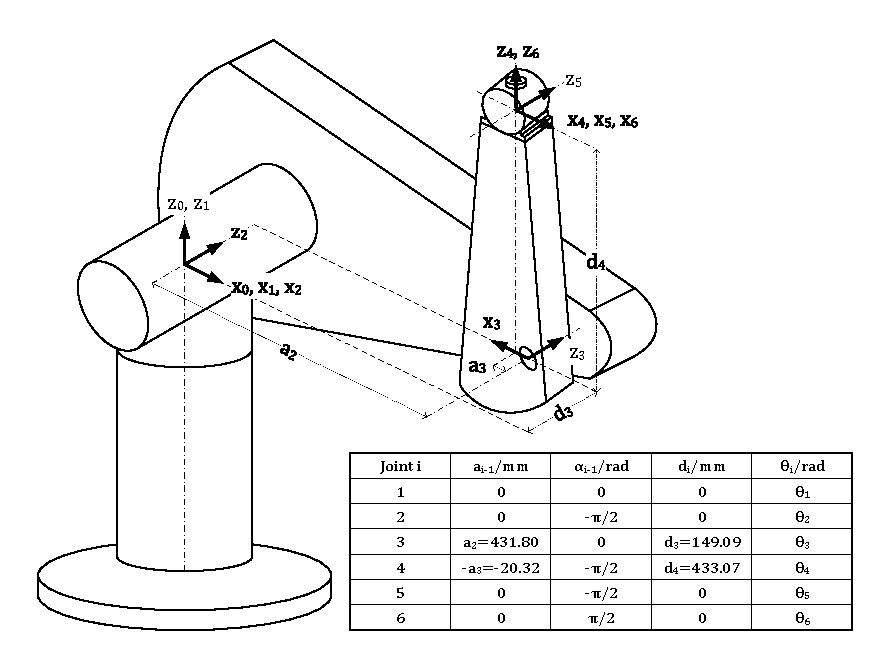
\includegraphics[scale=1]{images//puma560_mdh.pdf} \\
	\caption{PUMA 560 机器人 MDH 模型}
	\label{puma560_mdh_model}
\end{figure}

根据 \ref{mdh_model_adjacent_link_forward_coordinate_transformation} 可求得每个连杆的变换矩阵:
\begin{flalign}
\begin{array}{ll}
{_1^0\bm{T}} = \begin{bmatrix}
	c_{\theta_1} & -s_{\theta_1} & 0 & 0 \\
	s_{\theta_1} & c_{\theta_1}  & 0 & 0 \\
	0            & 0             & 1 & 0 \\
	0            & 0             & 0 & 1
\end{bmatrix}, &
{_2^1\bm{T}} = \begin{bmatrix}
	c_{\theta_2}  & -s_{\theta_2} & 0 & 0 \\
	0             & 0             & 1 & 0 \\
	-s_{\theta_2} & -c_{\theta_2} & 0 & 0 \\
	0             & 0             & 0 & 1
\end{bmatrix}, \\
{_3^2\bm{T}} = \begin{bmatrix}
	c_{\theta_3} & -s_{\theta_3} & 0 & a_2 \\
	s_{\theta_3} & c_{\theta_3}  & 0 & 0 \\
	0            & 0             & 1 & d_3 \\
	0            & 0             & 0 & 1
\end{bmatrix}, &
{_4^3\bm{T}} = \begin{bmatrix}
	c_{\theta_4}  & -s_{\theta_4} & 0 & -a_3 \\
	-s_{\theta_4} & -c_{\theta_4}  & 0 & d_4 \\
	0             & 0             & 1 & 0 \\
	0             & 0             & 0 & 1
\end{bmatrix}, \\
{_5^4\bm{T}} = \begin{bmatrix}
	c_{\theta_5}  & -s_{\theta_5} & 0 & 0 \\
	0             & 0             & 1 & 0 \\
	-s_{\theta_5} & -c_{\theta_5} & 0 & 0 \\
	0             & 0             & 0 & 1
\end{bmatrix}, &
{_6^5\bm{T}} = \begin{bmatrix}
	c_{\theta_6} & -s_{\theta_6} & 0  & 0 \\
	s_{\theta_6} & c_{\theta_6}  & -1 & 0 \\
	0            & 0             & 0  & 0 \\
	0            & 0             & 0  & 1
\end{bmatrix}.
\end{array}
\end{flalign}

那么由此可得连杆末端相对基坐标系的变换矩阵为:
\begin{equation}
\begin{aligned}
{_6^0\bm{T}} &= {_1^0\bm{T}}{_2^1\bm{T}}{_3^2\bm{T}}{_4^3\bm{T}}{_5^4\bm{T}}{_6^5\bm{T}} \\
&=\begin{bmatrix}
{_6^0\bm{n}} & {_6^0\bm{o}} & {_6^0\bm{a}} & {_6^0\bm{p}} \\
0            & 0            & 0            & 1
\end{bmatrix}
\end{aligned}
\end{equation}

点乘运算得到连杆末端姿态与位置为:
\begin{equation}\label{puma560_mdh_direct_kinematics_equations}
\begin{aligned}
{_6^0\bm{n}} &= \begin{bmatrix}
	s_1 (s_4 c_5 c_6 + c_4 s_6) + c_1 (s_{23} s_5 c_6 + c_{23} (c_4 c_5 c_6 - s_4 s_6)) \\
	s_1 s_{23} s_5 c_6 - c_1 (s_4 c_5 c_6 + c_4 s_6) + s_1 c_{23} (c_4 c_5 c_6 - s_4 s_6) \\
	(-s_{23} c_4 c_5 + c_{23} s_5)c_6 + s_{23} s_4 s_6
\end{bmatrix} \\
{_6^0\bm{o}} &= \begin{bmatrix}
	(s_1c_4-c_1c_{23}s_4)c_6-(s_1s_4c_5+c_1(c_{23}c_4c_5+s_{23}s_5))s_6 \\
	c_1(-c_4c_6+s_4c_5s_6)-s_1(s_{23}s_5s_6+c_{23}(s_4c_6+c_4c_5s_6)) \\
	s_{23}s_4c_6+(s_{23}c_4c_5-c_{23}s_5)s_6
\end{bmatrix} \\
{_6^0\bm{a}} &= \begin{bmatrix}
	s_1s_4s_5+c_1(-s_{23}c_5+c_{23}c_4s_5) \\
	-s_1s_{23}c_5+(s_1c_{23}c_4-c_1s_4)s_5 \\
	-c_{23}c_5-s_{23}c_4s_5
\end{bmatrix} \\
{_6^0\bm{p}} &= \begin{bmatrix}
	-s_1d_3+c_1(c_2a_2-c_{23}a_3-s_{23}d_4) \\
	c_1d_3+s_1(c_2a_2-c_{23}a_3-s_{23}d_4) \\
	-s_2a_2+s_{23}a_3-c_{23}d_4
\end{bmatrix}
\end{aligned}
\end{equation}

将广义坐标取具体数值计算末端执行器姿态并观察,即可验证以上变换矩阵是否正确。分别令 $\bm{q}$ 取不同广义坐标值,代入计算结果为:
\begin{flalign}
	{_6^0\bm{T}}\left(0,\ 0,\ 0,\ 0,\ 0,\ 0\right) &= \begin{bmatrix}
		1 & 0 & 0 & a_2 - d_3 \\
		0 & 1 & 0 & d_3 \\
		0 & 0 & 1 & d_4 \\
		0 & 0 & 0 & 1
	\end{bmatrix} \nonumber \\
	{_6^0\bm{T}}\left(0,\ 0,\ 0,\ \pi/2,\ 0,\ \pi/4\right) &= \begin{bmatrix}
	-\frac{1}{\sqrt{2}} & -\frac{1}{\sqrt{2}} & 0 & a_2 - d_3 \\
	\frac{1}{\sqrt{2}} & -\frac{1}{\sqrt{2}} & 0 & d_3 \\
	0 & 0 & 1 & d_4 \\
	0 & 0 & 0 & 1
	\end{bmatrix} \nonumber \\
	{_6^0\bm{T}}\left(\pi/2,\ 0,\ \pi/2,\ 0,\ 0,\ 0\right) &= \begin{bmatrix}
		0  & -1 & 0 & -d_3 \\
		0  & 0  & 1 & a_2 + d_4 \\
		-1 & 0  & 0 & a_3 \\
		0  & 0  & 0 & 1
	\end{bmatrix} \nonumber \\
	{_6^0\bm{T}}\left(\pi/2,\ 0,\ \pi/2,\ \pi/2,\ 0,\ \pi/4\right) &= \begin{bmatrix}
	-\frac{1}{\sqrt{2}} & \frac{1}{\sqrt{2}} & 0 & - d_3 \\
	0 & 0 & 1 & a_2 + d_4 \\
	\frac{1}{\sqrt{2}} & \frac{1}{\sqrt{2}} & 0 & a3 \\
	0 & 0 & 0 & 1
\end{bmatrix} \nonumber
\end{flalign}


\subsection{实例分析:Justin}

德国航空航天中心(简称DLR)研发的Justin七自由度机械臂,它的三个外侧关节具有两种可能构型,各相邻关节轴相交且垂直(见图 \ref{justin_mdh_model})。

\begin{figure}[htbp]
	\centering
	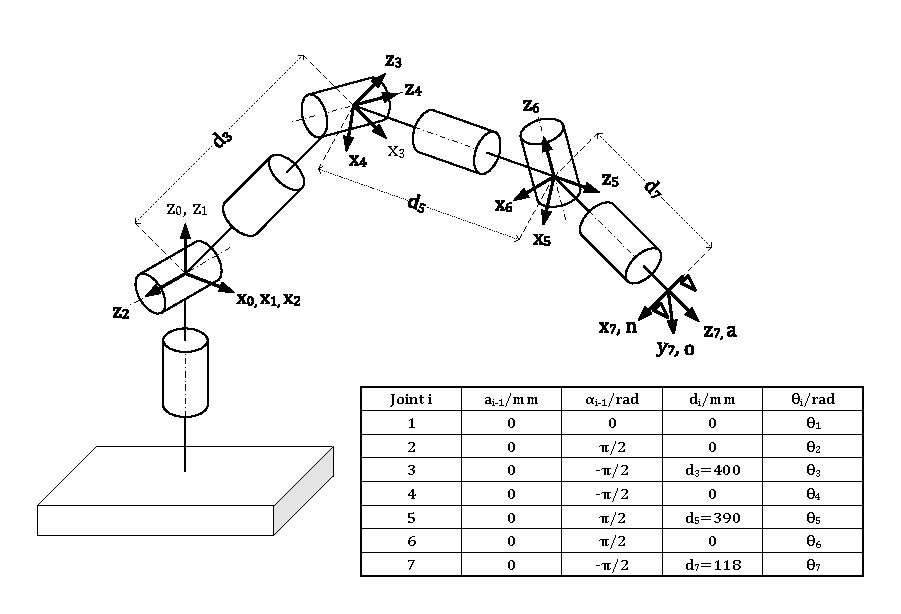
\includegraphics[scale=1]{images//dlr_justin_mdh.pdf} \\
	\caption{DLR Justin 机器人 MDH 模型}
	\label{justin_mdh_model}
\end{figure}

根据 \ref{mdh_model_adjacent_link_forward_coordinate_transformation} 计算每个连杆的变换矩阵:
\begin{flalign}
	\begin{array}{ll}
		{_1^0\bm{T}} = \begin{bmatrix}
			c_{\theta_1} & -s_{\theta_1} & 0 & 0 \\
			s_{\theta_1} & c_{\theta_1}  & 0 & 0 \\
			0            & 0             & 1 & 0 \\
			0            & 0             & 0 & 1
		\end{bmatrix}, &
		{_2^1\bm{T}} = \begin{bmatrix}
			c_{\theta_2} & -s_{\theta_2} & 0  & 0 \\
			0            & 0             & -1 & 0 \\
			s_{\theta_2} & c_{\theta_2}  & 0  & 0 \\
			0            & 0             & 0  & 1
		\end{bmatrix}, \\
		{_3^2\bm{T}} = \begin{bmatrix}
			c_{\theta_3}  & -s_{\theta_3} & 0 & 0 \\
			0             & 0             & 1 & d_3 \\
			-s_{\theta_3} & -c_{\theta_3} & 0 & 0 \\
			0             & 0             & 0 & 1
		\end{bmatrix}, &
		{_4^3\bm{T}} = \begin{bmatrix}
			c_{\theta_4}  & -s_{\theta_4} & 0 & 0 \\
			0             & 0             & 1 & 0 \\
			-s_{\theta_4} & -c_{\theta_4} & 0 & 0 \\
			0             & 0             & 0 & 1
		\end{bmatrix}, \\
		{_5^4\bm{T}} = \begin{bmatrix}
			c_{\theta_5} & -s_{\theta_5} & 0  & 0 \\
			0            & 0             & -1 & -d_5 \\
			s_{\theta_5} & c_{\theta_5}  & 0  & 0 \\
			0            & 0             & 0  & 1
		\end{bmatrix}, &
		{_6^5\bm{T}} = \begin{bmatrix}
			c_{\theta_6} & -s_{\theta_6} & 0  & 0 \\
			0            & 0             & -1 & 0 \\
			s_{\theta_6} & c_{\theta_6}  & 0  & 0 \\
			0            & 0             & 0  & 1
		\end{bmatrix}, \\
		{_7^6\bm{T}} = \begin{bmatrix}
			c_{\theta_7}  & -s_{\theta_7} & 0 & 0 \\
			0             & 0             & 1 & d_7 \\
			-s_{\theta_7} & -c_{\theta_7} & 0 & 0 \\
			0             & 0             & 0 & 1
		\end{bmatrix}.
	\end{array}
\end{flalign}

那么由此可得连杆末端相对基坐标系的变换矩阵为:
\begin{equation}
	\begin{aligned}
		{_7^0\bm{T}} &= {_1^0\bm{T}}{_2^1\bm{T}}{_3^2\bm{T}}{_4^3\bm{T}}{_5^4\bm{T}}{_6^5\bm{T}}{_7^6\bm{T}} \\
		&=\begin{bmatrix}
			{_7^0\bm{n}} & {_7^0\bm{o}} & {_7^0\bm{a}} & {_7^0\bm{p}} \\
			0            & 0            & 0            & 1
		\end{bmatrix}
	\end{aligned}
\end{equation}

点乘运算得到连杆末端姿态与位置为:
\begin{equation}\label{justin_mdh_direct_kinematics_equations}
	\begin{aligned}
		{_7^0\bm{n}} &= \begin{bmatrix}
			(({x_1}c_{5}-{x_3}s_{5})c_{6}+{x_2}s_{6})c_{7}-({x_1}s_{5}+{x_3}c_{5})s_{7} \\
			(({y_1}c_{5}-{y_3}s_{5})c_{6}+{y_2}s_{6})c_{7}-({y_1}s_{5}+{y_3}c_{5})s_{7} \\
			(({z_1}c_{5}-{z_3}s_{5})c_{6}+{z_2}s_{6})c_{7}-({z_1}s_{5}+{z_3}c_{5})s_{7}
		\end{bmatrix} \\
		{_7^0\bm{o}} &= \begin{bmatrix}
			-(({x_1}c_{5}-{x_3}s_{5})c_{6}+{x_2}s_{6})s_{7}-({x_1}s_{5}+{x_3}c_{5})c_{7} \\
			-(({y_1}c_{5}-{y_3}s_{5})c_{6}+{y_2}s_{6})s_{7}-({y_1}s_{5}+{y_3}c_{5})c_{7} \\
			-(({z_1}c_{5}-{z_3}s_{5})c_{6}+{z_2}s_{6})s_{7}-({z_1}s_{5}+{z_3}c_{5})c_{7}
		\end{bmatrix} \\
		{_7^0\bm{a}} &= \begin{bmatrix}
			-({x_1}c_{5}-{x_3}s_{5})s_{6}+{x_2}c_{6} \\
			-({y_1}c_{5}-{y_3}s_{5})s_{6}+{y_2}c_{6} \\
			-({z_1}c_{5}-{z_3}s_{5})s_{6}+{z_2}c_{6}
		\end{bmatrix} \\
		{_7^0\bm{p}} &= \begin{bmatrix}
			-{p_1}{d_3}+{x_2}{d_5}-(({x_1}c_{5}-{x_3}s_{5})s_{6}-{x_2}c_{6}){d_7} \\
			-{p_2}{d_3}+{y_2}{d_5}-(({y_1}c_{5}-{y_3}s_{5})s_{6}-{y_2}c_{6}){d_7} \\
			{p_3}{d_3}+{z_2}{d_5}-(({z_1}c_{5}-{z_3}s_{5})s_{6}-{z_2}c_{6}){d_7}
		\end{bmatrix}
	\end{aligned}
\end{equation}
其中,
\begin{equation}
\begin{aligned}
{x_1} &= ((c_{1}c_{2}c_{3}-s_{1}s_{3})c_{4}+c_{1}s_{2}s_{4}) \\
{x_2} &= ((c_{1}c_{2}c_{3}-s_{1}s_{3})s_{4}-c_{1}s_{2}c_{4}) \\
{x_3} &= (c_{1}c_{2}s_{3}+s_{1}c_{3}) \\
{y_1} &= ((s_{1}c_{2}c_{3}+c_{1}s_{3})c_{4}+s_{1}s_{2}s_{4}) \\
{y_2} &= ((s_{1}c_{2}c_{3}+c_{1}s_{3})s_{4}-s_{1}s_{2}c_{4}) \\
{y_3} &= (s_{1}c_{2}s_{3}-c_{1}c_{3}) \\
{z_1} &= (s_{2}c_{3}c_{4}-c_{2}s_{4}) \\
{z_2} &= (s_{2}c_{3}s_{4}+c_{2}c_{4}) \\
{z_3} &= s_{2}s_{3} \\
{p_1} &= c_{1}s_{2} \\
{p_2} &= s_{1}s_{2} \\
{p_3} &= c_{2}
\end{aligned}
\end{equation}

将广义坐标取具体数值计算末端执行器姿态并观察,即可验证以上变换矩阵是否正确。分别令 $\bm{q}$ 取不同广义坐标值,代入计算结果为:
\begin{flalign}
	{_7^0\bm{T}}\left(0,\ 0,\ 0,\ 0,\ 0,\ 0,\ 0\right) &= \begin{bmatrix}
		1 & 0 & 0 & d_3+d_5+d_7 \\
		0 & 1 & 0 & 0 \\
		0 & 0 & 1 & 0 \\
		0 & 0 & 0 & 1
	\end{bmatrix} \nonumber \\
	{_7^0\bm{T}}\left(0,\ 0,\ 0,\ 0,\ \pi/2,\ \pi/6,\ \pi/4\right) &= \begin{bmatrix}
		-\frac{\sqrt{2}}{2} & -\frac{\sqrt{2}}{2} & 0 & 0 \\
		\frac{\sqrt{6}}{4} & -\frac{\sqrt{6}}{4} & -\frac{1}{2} & -\frac{1}{2}d_7 \\
		\frac{\sqrt{2}}{4} & -\frac{\sqrt{2}}{4} & \frac{\sqrt{3}}{2} & d_3+d_5+\frac{\sqrt{3}}{2}d_7 \\
		0 & 0 & 0 & 1
	\end{bmatrix} \nonumber \\
	{_7^0\bm{T}}\left(0,\ -\pi/2,\ 0,\ -\pi/2,\ 0,\ 0,\ 0\right) &= \begin{bmatrix}
		1 & 0 & 0 & d_3 \\
		0 & 1 & 0 & 0 \\
		0 & 0 & 1 & d_5+d_7 \\
		0 & 0 & 0 & 1
	\end{bmatrix} \nonumber \\
	{_7^0\bm{T}}\left(0,\ -\pi/2,\ 0,\ -\pi/2,\ \pi/2,\ \pi/6,\ \pi/4\right) &= \begin{bmatrix}
		-\frac{\sqrt{2}}{2} & -\frac{\sqrt{2}}{2} & 0 & d_3 \\
		\frac{\sqrt{6}}{4} & -\frac{\sqrt{6}}{4} & -\frac{1}{2} & -\frac{1}{2}d_7 \\
		\frac{\sqrt{2}}{4} & -\frac{\sqrt{2}}{4} & \frac{\sqrt{3}}{2} & d_5+\frac{\sqrt{3}}{2}d_7 \\
		0 & 0 & 0 & 1
	\end{bmatrix} \nonumber
\end{flalign}


\section{运动学标定}

系统精度与高精度的正运动学参数密不可分,运动学标定技术通过系统的测量机械臂末端执行器位姿数据精确估算运动学 DH 参数,运动学标定技术不会直接测量系统结构的几何参数。

机械臂系统中,对于转动关节 $q_i=\theta_i$,对于移动关节 $q_i=d_i$,末端执行器位姿取决于关节变量,因此正运动学方程也可以表示为\textbf{操作空间}位姿向量 $\bm{x}_e$ 关于\textbf{关节空间}向量 $\bm{q}$ 的函数 $\bm{k}$:
\begin{equation}
\begin{aligned}
	\bm{x}_e &= \left(\bm{\phi}_e , \bm{p}_e\right) = \left(\bm{n} , \bm{o} , \bm{a} , \bm{p}\right)\text{,操作空间位置与姿态向量} \\
	&=\bm{k} \left(q_1 , \cdots , q_n\right) \text{,关节空间向量}
\end{aligned}
\end{equation}

为考察操作空间变量与运动学 DH 参数间的关系,正运动学方程还可以表示为:
\begin{equation}
	\begin{aligned}
		\bm{x}_e =\bm{k} \left(\bm{a},\bm{\alpha},\bm{d},\bm{\theta}\right)
	\end{aligned}
\end{equation}

为有效完成运动学标定,需高精度完成机械臂位姿测量,可使用辅助机械电子装置,将末端执行器按限制在已知精度的给定位姿。另外,也可以使用直接测量系统,采用三角测量技术测量目标在笛卡尔空间的位置和方向。

令 $\bm{x}_m$ 为测量的位姿,$\bm{x}_n$ 为用参数 $\left(\bm{a},\bm{\alpha},\bm{d},\bm{\theta}\right)$ 的标称值计算而来的标称位姿值。假设固定参数标称值和机械结构的设计数据相等,关节变量的标称值与机械结构处于给定位姿时传感器提供的数据相等。那么,偏差 $\delta \bm{x} = \bm{x}_m - \bm{x}_n$ 则为给定位姿时对精度的度量。假设偏差值相对较小,那么近似有如下关系:
\begin{equation}
	\begin{aligned}
	\Delta\bm{x} = \frac{\partial\bm{k}}{\partial\bm{a}} \Delta\bm{a} + \frac{\partial\bm{k}}{\partial\bm{\alpha}} \Delta\bm{\alpha} + \frac{\partial\bm{k}}{\partial\bm{d}} \Delta\bm{d} + \frac{\partial\bm{k}}{\partial\bm{\theta}} \Delta\bm{\theta}
\end{aligned}
\end{equation}
其中 $\left(\Delta\bm{a},\Delta\bm{\alpha},\Delta\bm{d},\Delta\bm{\theta}\right)$ 表示真实结构参数值与标称值之间的偏差。$\left({\partial\bm{k}}/{\partial\bm{a}},{\partial\bm{k}}/{\partial\bm{\alpha}},{\partial\bm{k}}/{\partial\bm{d}},{\partial\bm{k}}/{\partial\bm{\theta}}\right)$ 为 $ m \times n$ 偏导矩阵,其元素为正运动学方程分量关于单个参数的偏导数。

将参数合成为一个 $4n \times 1$ 向量 $\bm{\zeta} = {\left[ \bm{a}^T \quad \bm{\alpha}^T \quad \bm{d}^T \quad \bm{\theta}^T \right]}^T$。令 $\Delta\bm{\zeta} = \bm{\zeta}_m - \bm{\zeta}_n$ 表示参数关于标称值的偏差,$\bm{\varPhi} = \left[{\partial\bm{k}}/{\partial\bm{a}} \quad {\partial\bm{k}}/{\partial\bm{\alpha}} \quad {\partial\bm{k}}/{\partial\bm{d}} \quad {\partial\bm{k}}/{\partial\bm{\theta}}\right]$ 为计算参数 $\bm{\zeta}_n$ 的标称值的 $m \times 4n$ 运动学标定矩阵。那么上述近似等式可简写为:
\begin{equation}
	\begin{aligned}
		\Delta\bm{x} = \bm{\varPhi}\left(\bm{\zeta}_n\right)\Delta\bm{\zeta}
	\end{aligned}
\end{equation}
目标是从 $\bm{\zeta}_n$,$\bm{x}_n$ 的信息和 $\bm{x}_m$ 测量值计算出 $\Delta\bm{\zeta}$。上式为包含 $4n$ 个未知数,$m$ 个方程的方程组,其中 $m<4n$,因此必须对末端执行器的位姿进行足够数量的测量,进而得到至少包含 $4n$ 个方程的方程组。若对 $l$ 个位姿进行测量,那么可以得出:
\begin{equation}\label{kinematic_calibration_formula}
\Delta\bar{\bm{x}} = \begin{bmatrix} \Delta\bm{x}_1 \\ \vdots \\ \Delta\bm{x}_l \end{bmatrix} = \begin{bmatrix} \Delta\bm{\varPhi}_1 \\ \vdots \\ \Delta\bm{\varPhi}_l \end{bmatrix} \Delta\bm{\zeta} = \bar{\bm{\varPhi}}\Delta\bm{\zeta}
\end{equation}

计算 $\bm{\varPhi}_i$ 所需参数标称值为结构几何常量,广义关节变量由所处位姿决定。为了避免矩阵 $\bar{\bm{\varPhi}}$ 的病态情况,选择 $l$ 时需满足 $lm >> 4n$,然后采用最小二乘法求解式 \ref{kinematic_calibration_formula},此时解的形式为:
\begin{equation}
	\Delta\bm{\zeta} = (\bar{\bm{\varPhi}}^T\bar{\bm{\varPhi}})^{-1}\bar{\bm{\varPhi}}^T\Delta\bar{\bm{x}}
\end{equation}
通过用参数 $\Delta\bm{\zeta}$ 的理论标称值计算 $\bar{\bm{\varPhi}}$,第一个参数估计由下式给出:
\begin{equation}
\bm{\zeta}'=\bm{\zeta}_n + \Delta\bm{\zeta}
\end{equation}
这是非线性参数估计问题,通过逐次迭代指导 $\Delta\bm{\zeta}$ 收敛到指定值。每次迭代过程中,通过上一步迭代得到的 $\bm{\zeta}'$ 计算更新标定矩阵 $\bar{\bm{\varPhi}}$,而偏差 $\Delta\bar{\bm{x}}$ 使用末端执行器的 $l$ 组位姿测量值与上一步迭代得到的参数值通过正运动学方程计算得到位姿值之差进行计算。通过运动学标定,可获得机械臂几何参数更精确的估计值,并对关节传感器测量值进行更精确的修正。实际应用中还可以在测量系统启动中采用其他标定方法保证位姿传感器数据与机械臂实际姿态相一致,例如,在增量式位置传感器中,可将机械机构调整到给定的参考位姿,然后用相应位姿值初始化传感器。



\section{逆运动学}\label{inverse_kinematics}

逆运动学研究的问题是:一直工具坐标系相对于固定坐标系的期望位姿,计算满足该期望位姿的广义关节坐标值。求解你运动学问题分为两步:首先,坐标变换求解相对于基坐标系 $\left\{B\right\}$ 的腕部坐标系 $\left\{W\right\}$;然后,采用逆运动学方法求解广义关节坐标 $\bm{q}$。


\begin{property}{\textbf{逆解存在性}}
若逆解存在,则被指定的目标点必须在工作空间内。实际机械机构中关节不是总能旋转整圈,此时工作空间范围或可达姿态数目会减少。当操作臂小于六个自由度时,不能到达三维空间一般性目标位姿;当操作臂至少六个自由度时,若腕部坐标系的期望位姿在工作空间内,那么至少存在一个逆解。
\end{property}


\begin{property}{\textbf{逆解多解性}}
机械臂自由度可能会大于工作空间自由度,而且超越函数存在多解性,因此系统会出现多解的情况,而实际系统只会选择某个解,选择标准一般是就近原则,但存在障碍的情况下,若较劲解会发生碰撞,则只能选择相对较远的解。

解得个数不仅取决于关节数,而且还是连杆参数和关节运动范围的函数。通常,连杆的非零参数越多,解的最大数目也越大,到达特定目标的方式也越多,对于 $6$ 个旋转关节的机械臂,最多可能有 $16$ 个解。
\end{property}

由大量超越函授构成的运动学方程没有通用解法,不同的系统机构解的形式不同。若关节变量能够通过某种算法确定,且通过这种算法可以计算出已知位姿相对应的\textbf{全部关节变量},那么机械臂是可解的。机械臂的全部求解方法可分为两大类:\textbf{解析解}(即封闭解)和\textbf{数值解}。数值解一般采用数值迭代程序进行求解,多解情况下不能保证求出全部的解,而且其求解速度较慢。理想情况是可以设计出由解析解的机械臂系统。解析解求解方法有两大类:代数法和几何法。代数法求解运动学方程是将给定的方程转换为根据已知条件可求解的形式,几何法求解运动方程则将机械臂的空间几何参数分解为平面几何问题。


关于运动学求解方面业界目前的一个主要研究成果是:所有包含转动关节和移动关节的串联型六自由度机构均是可解的。但一般是数值解,只有机构存在几个正交关节轴或有多个关节轴夹角为零或 $\pm 90^{\circ}$ 时存在解析解,六个旋转关节机械臂存在解析解的充分条件是相邻的三个关节轴相交(相互垂直或平行)于一点。


\subsection{低自由度机械臂子空间}

机械臂可达工作空间是其自由度子空间的子集。确定 $n$ 自由度机械臂子空间的常用方法是给出其末端腕部或工具坐标系表达式,该表达式含有 $n$ 个变量,若所有这些变量均是自由变量,那么它们所有取值的集合就构成了 $n$ 自由度机械臂的子空间。通常采用 $n$ 个参数来定义具有 $n$ 个自由度的机械臂的目标点。例如若给定 $6$ 自由度的目标位置,一般情况下自由度小于 $6$ 的机械臂无法到达该点,这种情况下,可在该机械臂子空间内的可达工作空间寻找\textbf{可达目标位置}尽可能和\textbf{期望目标位置}接近。


\subsection{三轴相交求解方法}

一般构型的六自由度机器人没有解析解,但某些特殊构型情况下是可解的。三个连续轴相较于一点的六自由度机械臂是可解的,例如很多商业机器人采用六个旋转关节且后三轴相较于一点的机械臂。

当最后三轴相交时,连杆坐标系 $\left\{4\right\}$、$\left\{4\right\}$ 和 $\left\{4\right\}$ 的原点均位于交点,该点相对于基坐标系表示为:
\begin{equation}
{^0\bm{P_{4_o}}} = {_1^0\bm{T}}{_2^1\bm{T}}{_3^2\bm{T}}{^3\bm{P_{4_o}}} = \begin{bmatrix}
x \\
y \\
z \\
1
\end{bmatrix}
\end{equation}
或,当 $i=4$ 时,由式 $\ref{mdh_model_adjacent_link_forward_coordinate_transformation}$ 第四列有
\begin{equation}
	{^0\bm{P_{4_o}}} = {_1^0\bm{T}}{_2^1\bm{T}}{_3^2\bm{T}}\begin{bmatrix}
		a_3 \\
		-d_4s_{\alpha_3} \\
		d_4c_{\alpha_3} \\
		1
	\end{bmatrix}
\end{equation}
或
\begin{equation}
	{^0\bm{P_{4_o}}} = {_1^0\bm{T}}{_2^1\bm{T}}\begin{bmatrix}
		f_1\left(\theta_3\right) \\
		f_2\left(\theta_3\right) \\
		f_3\left(\theta_3\right) \\
		1
	\end{bmatrix}
\end{equation}
式中
\begin{equation}
\begin{bmatrix}
f_1 \\
f_2 \\
f_3 \\
1
\end{bmatrix} = {_3^2\bm{T}}\begin{bmatrix}
a_3 \\
-d_4s_{\alpha_3} \\
d_4c_{\alpha_3} \\
1
\end{bmatrix}
\end{equation}
对以上式中的 ${_3^2\bm{T}}$ 应用式 \ref{mdh_model_adjacent_link_forward_coordinate_transformation} 可将 $f$ 表示为:
\begin{equation}
\begin{aligned}
	f_1 &= a_3c_3 + d_4s_{\alpha_3}s_3 + a_2 \\
	f_2 &= a_3c_{\alpha_2}s_3 - d_4s_{\alpha_3}c_{\alpha_2}c_3 - d_4s_{\alpha_2}c_{\alpha_3} - d_3s_{\alpha_2} \\
	f_3 &= a_3s_{\alpha_2}s_3 - d_4s_{\alpha_3}s_{\alpha_2}c_3 + d_4c_{\alpha_2}c_{\alpha_3} + d_3c_{\alpha_2}
\end{aligned}
\end{equation}
对以上式中的 ${_1^0\bm{T}}$ 和 ${_2^1\bm{T}}$ 应用式 \ref{mdh_model_adjacent_link_forward_coordinate_transformation} 可得到:
\begin{equation}
	{^0\bm{P_{4_o}}} = \begin{bmatrix}
		c_1g_1 - s_1g_2 \\
		s_1g_1 - c_1g_2 \\
		g_3 \\
		1
	\end{bmatrix}
\end{equation}
式中
\begin{equation}
\begin{aligned}
g_1 &= c_2f_1 - s_2f_2 + a_1 \\
g_2 &= s_2c_{\alpha_1}f_1 + c_2c_{\alpha_1}f_2 - s_{\alpha_1}f_3 - d_2s_{\alpha_1} \\
g_2 &= s_2s_{\alpha_1}f_1 + c_2s_{\alpha_1}f_2 + c_{\alpha_1}f_3 + d_2c_{\alpha_1}
\end{aligned}
\end{equation}
计算 ${^0\bm{P_{4_o}}}$ 绝对值平方的表达式,这里 $r=x^2 + y^2 + z^2$,从而消去 $\theta_1$,故有:
\begin{equation}
\begin{aligned}
r &= g_1^2 + g_2^2 + g_3^2 \\
&= f_1^2 + f_2^2 + f_3^2 + a_1^2 + d_2^2 + 2d_2f_3 + 2a_1(c_2f_1 - s_2f_2)
\end{aligned}
\end{equation}
列出 $Z$ 方向分量方程,并改写出两个方程:
\begin{equation}
\begin{aligned}
r &= 2\alpha_1\left(k_1c_2 + k_2s_2 \right) + k_3 \\
z &= s_{\alpha_1}\left(k_1s_2 + k_2c_2 \right) + k_4
\end{aligned}
\end{equation}
式中
\begin{equation}
	\begin{aligned}
		k_1 &= f_1 \\
		k_2 &= -f_2 \\
		k_3 &= f_1^2 + f_2^2 + f_3^2 + a_1^2 + d_2^2 + 2d_2f_3 \\
		k_4 &= c_{\alpha_1}f_3 + d_2c_{\alpha_1}
	\end{aligned}
\end{equation}
上式以消去因变量 $\theta_1$,只包括 $\theta_2$ 和 $\theta_3$,据此可求解 $\theta_3$,具体分以下情况:
\begin{enumerate}
	\item 若 $a_1=0$,则 $r=k_3$,其中 $r$ 已知,$k_3$ 是关于 $\theta_3$ 的函数,可用三角函数万能公式代换为包含 $\tan(\theta_3/2)$ 的二次方程进而解出 $\theta_3$。
	\item 若 $s_{\alpha_1}=0$,则 $z=k_4$,其中 $z$ 已知,$k_4$ 是关于 $\theta_3$ 的函数,同样的方法可解出 $\theta_3$。
	\item 此外,可通过上述的 $r$、$k$ 方程组消去 $\theta_2$,得到:
	\begin{equation}
		\frac{(r-k_3)^2}{4a_1^2} + \frac{(z-k_4)^2}{s_{a_1}^2} = k_1^2 + k_2^2
	\end{equation}
	可用三角函数万能公式代换得到四次方程解出 $\theta_3$。解出 $\theta_3$ 后代入 $r$、$k$ 方程组解出 $\theta_2$,进而解出 $\theta_1$。
\end{enumerate}

最后需要求解 $\theta_4$、$\theta_5$和$\theta_6$。由于最后三轴相交,故这些关节角只影响末端连杆的方向,只需通过 ${^0_6}T$ 的旋转分量即可完成关节角计算。已知 $\theta_1$、$\theta_2$和$\theta_3$,并令  $\theta_4 = 0$,即可计算出 $^0_4R$,连杆坐标系 $\left\{6\right\}$ 与 $\left\{4\right\}$ 方向的差别仅在于最后三个关节的作用。由于 ${^0_6}R$ 已知,故有:
\begin{equation}
	{^4_6}R \lvert_{\theta_4 = 0} = {^0_4}R^{-1}\lvert_{\theta_4 = 0} {^0_6}R
\end{equation}


\subsection{机械臂求解}
可以将工具坐标系 $\left\{T\right\}$ 和 固定坐标系 $\left\{S\right\}$ 应用于逆运动学求解。已知${^B_S}T$、${^S_T}T$和${^W_T}T$,则可解得相对于基坐标系 $\left\{B\right\}$ 的腕部坐标系 $\left\{W\right\}$:
\begin{equation}
	{^B_W}T = {^B_S}T {^S_T}T {^W_T}T^{-1}
\end{equation}
以 ${^B_W}T$ 作为逆运动学输入即可计算各个广义坐标。


\subsection{重复精度与精度}
成熟的工业机器人产品一般可以运动到达的示教的目标点,该点是机器人运动实际要达到的点,同时关节位置传感器读取存储关节位置;当命令机器人返回该点时,每个关节都移动到已存储的关节位置。这种场景中因为没有在直角坐标系中指定目标点,仅仅是简单的示教运动再现,不存在逆运动学问题。当需要确定机械臂返回示教点的精度时即在确定机械臂的\textbf{重复精度}。

当目标位姿是在笛卡尔坐标系中指定时,则需求解逆运动学,计算关节变量。这种场景中,可以将操作臂移动到未曾示教或未曾到达过的点,称之为\textbf{计算点},到达这个计算点的精度即为机械臂的\textbf{精度}。机械臂的精度不会超过其重复精度,精度受运动学参数精度影响,这些参数误差会引起逆运动学关节变量计算误差。因此尽管绝大多数工业机器人重复精度很高,但精度却较差,并且不同机械臂之间精度相差相当大。通过对操作臂运动学参数辨识和标定技术可以提高操作臂精度。


\subsection{计算问题}
许多路径控制方法需要以很高的速率计算机械臂的逆运动学问题,比如 30 Hz 或更快,因此提高计算效率具有重要意义。正运动学中相关方法也适用于逆运动学,而逆运动学中特有的\textbf{反正切查表法}可以有效提高计算效率。多解的情况下,计算结构非常重要,\textbf{并行计算}所有的解可以大幅提高计算效率。使用几何法求解逆运动学问题时,在计算出第一个解后,有时可通过对各种角度做简单操作来计算多解问题,即第一个接计算比较费时,但可以通过计算角度的和差或加减 $\pi$ 等三角方法可以很快求得其余解。


\subsection{实例分析:PUMA 560}
本例介绍 PUMA 560 机械臂逆运动学代数解法,适用于常见 6 自由度机械臂。已知 ${^0_6}T$,那么有:
\begin{equation}
	{^0_6}T = \begin{bmatrix}
		r_{11} & r_{12} & r_{13} & p_x \\
		r_{21} & r_{22} & r_{23} & p_y \\
		r_{31} & r_{32} & r_{33} & p_z \\
		0      & 0      & 0      & 1
	\end{bmatrix} = {^0_1}T\left(\theta_1\right) {^1_2}T\left(\theta_2\right) {^2_3}T\left(\theta_3\right) {^3_4}T\left(\theta_4\right) {^4_5}T\left(\theta_5\right) {^5_6}T\left(\theta_6\right)
\end{equation}
上式\textbf{两侧同时乘以 ${^0_1}T\left(\theta_1\right)$ 的逆变换即可分离关节变量 $\theta_1$},即:
\begin{equation}\label{puma560_ik_theta_1_equation}
	\begin{aligned}
		&\begin{bmatrix}
			c_{\theta_1} & -s_{\theta_1} & 0 & 0 \\
			s_{\theta_1} & c_{\theta_1}  & 0 & 0 \\
			0            & 0             & 1 & 0 \\
			0            & 0             & 0 & 1
		\end{bmatrix}
		\begin{bmatrix}
			r_{11} & r_{12} & r_{13} & p_x \\
			r_{21} & r_{22} & r_{23} & p_y \\
			r_{31} & r_{32} & r_{33} & p_z \\
			0      & 0      & 0      & 1
		\end{bmatrix} = {^1_6}T\left(\bm{\theta}\right)
	\end{aligned}
\end{equation}
展开即:
\begin{equation}
	\begin{aligned}
		&\begin{bmatrix}
			c_1r_{11}-s_1r_{21} & c_1r_{12}-s_1r_{22} & c_1r_{13}-s_1r_{23} & c_1p_x-s_1p_y \\
			s_1r_{11}+c_1r_{21} & s_1r_{12}+c_1r_{22} & s_1r_{13}+c_1r_{23} & s_1p_x+c_1p_y \\
			r_{31}              & r_{32}              & r_{33}              & p_z \\
			0                   & 0                   & 0                   & 1
		\end{bmatrix} \nonumber = \\
		&\left[
		\begin{array}{cc}
			-s_{23}s_5c_6+c_{23}(c_4c_5c_6-s_4s_6) & s_{23}s_5s_6-c_{23}(c_4c_5s_6+s_4c_6) \\
			s_{4}c_5c_6+c_4s_6 & c_{4}c_6-s_4c_5s_6 \\
			-(s_{23}c_4c_5+c_{23}s_5)c_6+s_{23}s_4s_6 & s_{23}s_4c_6+(s_{23}c_4c_5+c_{23}s_5)s_6 \\
			0            & 0
		\end{array}
		\right. \\
		&\left.
		\begin{array}{cc}
			s_{23}c_5+c_{23}c_4s_5 & c_2a_2-c_{23}a_3+s_{23}d_4 \\
			s_4s_5 & d_3 \\
			c_{23}c_5-s_{23}c_4s_5 & -s_2a_2+s_{23}a_3+c_{23}d_4 \\
			0 & 1
		\end{array}
		\right]
	\end{aligned}
\end{equation}
令上述方程式两边元素 $(2,4)$ 相等,则有:
\begin{equation}
	s_1p_x+c_1p_y = d_3
\end{equation}
运用三角参数方程恒等变换,令:
\begin{equation}
	\begin{aligned}
		p_x = r\cos\phi \\
		p_y = r\sin\phi
	\end{aligned}
\end{equation}
则有
\begin{equation}
	\begin{aligned}
		s_1\cos\phi+c_1\sin\phi &= \frac{d_3}{r} \\
	\xLongrightarrow{\text{积化和差}}
	\left\{
	\begin{aligned}
		\sin\left(\theta_1+\phi\right) &= \frac{d_3}{r} \\
		\cos\left(\theta_1+\phi\right) &= \pm\sqrt{1-\frac{d_3^2}{r^2}}
	\end{aligned}
	\right. 
	\xLongrightarrow{} \theta_1 &= \arctan\left(\pm\frac{d_3}{\sqrt{{r^2}-{d_3^2}}}\right)-\phi
	\end{aligned}
\end{equation}
其中
\begin{equation}
	\begin{aligned}
		r &= \sqrt{p_x^2+p_y^2} \\
		\phi &=\arctan \left(\frac{p_y}{p_x}\right)
	\end{aligned}
\end{equation}
如此已解得 $\theta_1$,即式 \ref{puma560_ik_theta_1_equation} 左边已知,令该式两边的元素 $(1,4)$ 和 $(3,4)$ 分别相等,则有:
\begin{equation}
\begin{aligned}
c_1p_x-s_1p_y &= c_2a_2-c_{23}a_3+s_{23}d_4 \\
p_z &= -s_2a_2+s_{23}a_3+c_{23}d_4
\end{aligned}
\end{equation}




\subsection{实例分析:ABB YUMI}





\section{微分运动学:雅可比矩阵}\label{differential_kinematics_jacobi_matrix}

微分运动学
微分运动学
微分运动学
微分运动学
微分运动学
微分运动学
微分运动学
微分运动学
微分运动学
微分运动学





\chapter{动力学}
机械臂动力学建模对运动仿真、机械臂机构分析和控制算法设计都有重要作用。机械臂仿真可在非真实物理系统环境下,实现最控制策略和运动规划技术的测试,动力学模型分析有助于机械臂模型的构造设计,计算实现典型运动需要的力和力矩,为关机机构、传动装置和执行器的设计提供有用信息。本章核心是两种在关节空间导出机械臂运动方程的方法。第一种方法基于拉格朗日方程,该方法建模简明、系统且通用;第二种方法基于牛顿-欧拉公式,建立一种递归模型,该方法计算效率高,便于计算机实现。

\begin{introduction}
	\item 拉格朗日方程
	\item 牛顿-欧拉公式
	\item 动力学正解与逆解
	\item 轨迹的动态标度
	\item 操作空间动力学模型
	\item 动力学可操作椭球
\end{introduction}


\section{拉格朗日方程}

拉格朗日方程建立了广义非保守力与关节位置、速度和加速度的关系,可以根据系统的动能和势能推导出动力学模型。

\begin{definition}{拉格朗日方程}{define_lagrange_func}
机械系统拉格朗日函数定义为系统总动能和势能之差:
\begin{equation}\label{robot_lagrange_func}
\mathcal{L} = \mathcal{K} - \mathcal{P}
\end{equation}
其中,动能 $\mathcal{K}$ 和势能 $\mathcal{P}$ 可用任何方便的坐标系表示。

对应的拉格朗日方程为:
\begin{equation}\label{robot_lagrange_kinematics_equation}
\frac{\mathrm{d}}{\mathrm{d}t} \frac{\partial \mathcal{L}}{\partial \dot{\bm{q}}} - \frac{\partial \mathcal{L}}{\partial \bm{q}} = \bm{\xi}
\end{equation}
其中,广义坐标 $\bm{q} = (q_1, q_2, ..., q_i ..., q_n)$ 是时间 $t$ 的函数,系统具有 $n$ 个自由度;广义力 $\bm{\xi}$ 是非保守力,如关节传动转矩、摩擦转矩一级由末端执行器对系统外作用力引起的关节转矩。
\end{definition}


\subsection{计算动能}

对于有 $n$ 级刚性连杆的机械臂,总动能为各个连杆和关节执行器动能分量的和:

\begin{equation}\label{total_kinetic_energy_of_rigid_manipulator}
	\mathcal{K} = \sum_{i = 1}^{n} \big( \mathcal{K}_{l_i} + \mathcal{K}_{m_i} \big)
\end{equation}
其中 $\mathcal{K}_{l_i}$ 为连杆 $i$ 的动能, $\mathcal{K}_{l_i}$ 为关节 $i$ 执行电机的动能。

连杆 $i$ 的动能分量为:
\begin{equation}\label{link_kinetic_energy_equation}
	\mathcal{K}_{l_i} = \frac{1}{2} \int_{V_{l_i}} { {{\bm{\dot p}}_{l_i}^{*T}} {{\bm{\dot p}}_{l_i}^*} \rho \mathrm{d}V }
\end{equation}
其中 $\dot{\bm{p}}_{l_i}^*$ 表示连杆上某质点 $P$ 的线速度向量,$\rho$ 为连杆体积微元 $\mathrm{d}V$ 的密度,$V_{l_i}$ 为连杆 $i$ 的体积。

一般情况下微元的位置向量 ${\bm{p}}_{l_i}^{*}$ 和连杆质心的位置向量 ${\bm{p}}_{l_i}$ 都在基坐标系中表示:
\begin{equation}
	\bm{r}_i = \left[ r_{ix} \ \ r_{iy} \ \ r_{iz} \right]^T = {\bm{p}}_{l_i}^* - \bm{p}_{l_i} \nonumber
\end{equation}
其中 $\bm{r}_i$ 为连杆质心到连杆上某质点 $P$ 的位置向量。而连杆质心在基坐标系中的位置向量 $\bm{p}_{l_i}$ 为:
\begin{equation}
\bm{p}_{l_i} = \frac{1}{m_{l_i}} \int_{V_{l_i}} {{{\bm{p}}_{l_i}^*} \rho \mathrm{d}V } \nonumber
\end{equation}
其中 $m_{l_i}$ 为连杆质量。进而可以计算得出该连杆上某质点 $P$ 的速度为:
\begin{equation}\label{particle_p_volocity_equation}
{\bm{\dot p}}_{l_i}^* = \bm{\dot p}_{l_i} + \bm{\omega}_i \times \bm{r}_i = \bm{\dot p}_{l_i} + {\bm{\mathcal{S}} \left(  \bm{\omega}_i \right) \bm{r}_i}
\end{equation}
其中 $\bm{\dot p}_{l_i}$ 为连杆质心线速度,$\bm{\omega}_i$ 为连杆角速度。将 \ref{particle_p_volocity_equation} 代入 \ref{link_kinetic_energy_equation} 中可求得各个连杆的动能,它由以下分量构成。

\textbf{平动分量} 可表示为:
\begin{equation}\label{link_kinetic_energy_translational_equation}
\mathcal{K}_t = \frac{1}{2} \int_{V_{l_i}} {{{\bm{\dot p}}_{l_i}^{*T}} {{\bm{\dot p}}_{l_i}^*} \rho \mathrm{d}V} = \frac{1}{2} m_{l_i} {{\bm{\dot p}}_{l_i}^{T}} {{\bm{\dot p}}_{l_i}}
\end{equation}

\textbf{牵连分量} 可表示为:
\begin{equation}
\begin{aligned}
\mathcal{K}_m &= 2 \cdot \frac{1}{2} \int_{V_{l_i}} {{{\bm{\dot p}}_{l_i}^{T}} {{\bm{\mathcal{S}} \left(  \bm{\omega}_i \right) \bm{r}_i}} \rho \mathrm{d}V} \\ 
&= {{\bm{\dot p}}_{l_i}^{T}} \bm{\mathcal{S}} \left(  \bm{\omega}_i \right) \int_{V_{l_i}} {\left( \bm{p}_{l_i}^* - \bm{p}_{l_i} \right) \rho \mathrm{d}V} \\
&= 0 \nonumber
\end{aligned}
\end{equation}

\textbf{旋转分量} 可表示为:
\begin{equation}\label{link_kinetic_energy_rotational_equation}
\begin{aligned}
\mathcal{K}_r &= \frac{1}{2} \int_{V_{l_i}} {\bm{r}_i^T {\bm{\mathcal{S}}^T \left(  \bm{\omega}_i \right)} {\bm{\mathcal{S}} \left(  \bm{\omega}_i \right)} \bm{r}_i \rho \mathrm{d}V}  \\
&= \frac{1}{2} \bm{\omega}_i^T \left( \int_{V_{l_i}} {{\bm{\mathcal{S}}^T \left( \bm{r}_i \right)} {\bm{\mathcal{S}} \left( \bm{r}_i \right)} \rho \mathrm{d}V} \right) \bm{w}_i \\
&= \frac{1}{2} \bm{\omega}_i^T \bm{I}_{l_i} \bm{\omega}_i
\end{aligned}
\end{equation}
其中:
\begin{equation}
\begin{aligned}
\bm{\mathcal{S}} \left( \bm{r}_i \right) = 
\begin{bmatrix}
0      & -r_{iz} & r_{iy} \\
r_{iz} & 0       & -r_{ix} \\
-r_{iy} & r_{ix}  & 0
\end{bmatrix}
\end{aligned}
\end{equation}

\begin{equation}
\begin{aligned}
\bm{I}_{l_i} &= 
\begin{bmatrix}
 \int {( r_{iy}^2 + r_{iz}^2) \rho \mathrm{d}V} & -\int {r_{ix} r_{iy} \rho \mathrm{d}V} & -{r_{ix} r_{iz} \rho \mathrm{d}V} \\
-\int {r_{ix} r_{iy} \rho \mathrm{d}V} &  \int {( r_{ix}^2 + r_{iz}^2) \rho \mathrm{d}V} & -{r_{iy} r_{iz} \rho \mathrm{d}V} \\
-\int {r_{ix} r_{iz} \rho \mathrm{d}V} & -{r_{iy} r_{iz} \rho \mathrm{d}V} &  \int {( r_{ix}^2 + r_{iy}^2) \rho \mathrm{d}V}
\end{bmatrix} \\
&= \begin{bmatrix}
 I_{{l_i}xx} & -I_{{l_i}xy} & -I_{{l_i}xz} \\
-I_{{l_i}xy} &  I_{{l_i}yy} & -I_{{l_i}yz} \\
-I_{{l_i}xz} & -I_{{l_i}yz} &  I_{{l_i}zz}
\end{bmatrix}
\end{aligned}
\end{equation}
对称矩阵 $\bm{I}_{l_i}$ 为基坐标系中表示的连杆 $i$ 质心的惯量,连杆的位置取决于机械臂位形,因此惯量由位形决定。若连杆 $i$ 的角速度在附着于连杆的坐标系中表示,那么角速度为:
$$ \bm{\omega}_i^i = \bm{R}_i^{-1} \bm{\omega}_i = \bm{R}_i^T \bm{\omega}_i $$
其中 $\bm{R}_i$ 是连杆 $i$ 相对基坐标系的旋转矩阵。参考连杆坐标系时惯量 $\bm{I}_{l_i}^i$ 为常量,那么参考基坐标系惯量可表示为:
\begin{equation}
\bm{I}_{l_i} = \bm{R}_i \bm{I}_{l_i}^i \bm{R}_i^{T}
\end{equation}

若连杆 $i$ 坐标系的轴与惯性中心轴一致,那么惯性积为零,与质心相关的惯量时对角矩阵。

对式动能的平移分量(式 \ref{link_kinetic_energy_translational_equation})和旋转分量(式 \ref{link_kinetic_energy_rotational_equation})求和得到该连杆的动能为:
\begin{equation}\label{link_kinetic_energy_cartesian_expression}
\begin{aligned}
\mathcal{K}_{l_i} &= \frac{1}{2} m_{l_i} {{\bm{\dot p}}_{l_i}^{T}} {{\bm{\dot p}}_{l_i}} + \frac{1}{2} \bm{\omega}_i^T \bm{I}_{l_i} \bm{\omega}_i \\
&= \frac{1}{2} m_{l_i} {{\bm{\dot p}}_{l_i}^{T}} {{\bm{\dot p}}_{l_i}} + \frac{1}{2} \bm{\omega}_i^T \bm{R}_i \bm{I}_{l_i}^i \bm{R}_i^T \bm{\omega}_i
\end{aligned}
\end{equation}

实际应用中很多时候将动能表示为系统广义坐标的函数,可通过将雅可比矩阵的计算方法应用在中间连杆上(而非末端执行器)求得:
\begin{flalign}
\bm{\dot p}_{l_i} &= {\bm{\jmath}_{P_1}^{l_i} \dot{q}_1} + {\bm{\jmath}_{P_2}^{l_i} \dot{q}_2} + ... + {\bm{\jmath}_{P_i}^{l_i} \dot{q}_i} = \bm{J}_P^{l_i} \bm{\dot q} \nonumber \\
\bm{\omega}_{l_i} &= {\bm{\jmath}_{O_1}^{l_i} \dot{q}_1} + {\bm{\jmath}_{O_2}^{l_i} \dot{q}_2} + ... + {\bm{\jmath}_{O_i}^{l_i} \dot{q}_i} = \bm{J}_O^{l_i} \bm{\dot q} \nonumber
\end{flalign}
其中当前连杆的雅可比矩阵为上式矩阵中与关节速度有关的列:
\begin{flalign}
\bm{J}_P^{l_i} &= \left[ \bm{\jmath}_{P_1}^{l_i} \quad \bm{\jmath}_{P_2}^{l_i} \quad ... \quad \bm{\jmath}_{P_i}^{l_i} \quad 0 \quad ... \quad 0 \right] \\
\bm{J}_O^{l_i} &= \left[ \bm{\jmath}_{O_1}^{l_i} \quad \bm{\jmath}_{O_2}^{l_i} \quad ... \quad \bm{\jmath}_{O_i}^{l_i} \quad 0 \quad ... \quad 0 \right]
\end{flalign}
上式中矩阵的列可由下面公式计算得出:
\begin{flalign}\label{link_jacobi_matrix_of_linear_and_angular_velocity}
\begin{bmatrix}
\bm{\jmath}_{P_j}^{l_i} \\
\bm{\jmath}_{O_j}^{l_i}
\end{bmatrix} = 
\begin{cases}
\begin{bmatrix}
\bm{z}_{j-1} \\
0
\end{bmatrix} & \text{移动关节,} \\ \\
\begin{bmatrix}
\bm{z}_{j-1} \times (\bm{p}_{l_i} - \bm{p}_{j-1}) \\
\bm{z}_{j-1} \\
\end{bmatrix} & \text{转动关节}
\end{cases}
\end{flalign}
其中 $\bm{p}_{j-1}$ 和 $\bm{z}_{j-1}$ 分别为坐标系 $j-1$ \textbf{原点的位置向量}和 $z$ \textbf{轴的单位向量},进而式 \ref{link_kinetic_energy_cartesian_expression} 中连杆的动能的广义坐标形式为:
\begin{flalign}\label{link_kinetic_energy_generalized_expression}
\mathcal{K}_{l_i} &= \frac{1}{2} m_{l_i} \bm{\dot q}^T (\bm{J}_P^{l_i})^T \bm{J}_P^{l_i} \bm{\dot q} + 
\frac{1}{2} \bm{\dot q}^T (\bm{J}_O^{l_i})^T \bm{R}_i \bm{I}_{l_i}^i \bm{R}_i^T \bm{J}_O^{l_i} \bm{\dot q}
\end{flalign}

关节电机的动量分量可通过与连杆相似的方式进行计算。以旋转电机为典型例子,假设电机所在连杆包含了电机固定部分(定子)的影响,那么此时只需考虑电机剩余部分的的单一影响。假设关节 $i$ 的电机位于连杆 $i-1$ 上。实际开环式运动系统的机械结构设计中,尽量将电机放在离机械臂底座尽可能近的地方,从而减轻运动链第一个关节的动态负载。电机通过机械传动装置提供关节驱动转矩,传动装置对动能的作用相应地包含在电机作用中。假设无诱导运动,即某关节的运动不会引起其他关节运动。

基于以上假设条件,电机转子 $i$ 的动能可表示为:
\begin{flalign}\label{motor_kinetic_energy_cartesion_expression}
\mathcal{K}_{m_i} &= \frac{1}{2} m_{m_i} {{\bm{\dot p}}_{m_i}^{T}} {{\bm{\dot p}}_{m_i}} + \frac{1}{2} \bm{\omega}_{m_i}^T  \bm{I}_{m_i} \bm{\omega}_{m_i}
\end{flalign}
其中 $m_{m_i}$ 是转子的质量,${\bm{\dot p}}_{m_i}$ 表示转子质心的线速度, $\bm{I}_{m_i}$ 是转子相对于质心的惯量,$\bm{\omega}_{m_i}$ 表示转子的角速度。

令 $\vartheta_{m_i}$ 表示转子角度位置,假设系统为刚性传动,那么有:
\begin{equation}
k_{ri} \dot{q}_i = \dot{\vartheta}_{m_i}
\end{equation}
其中 $k_{ri}$ 为齿轮减速比。移动关节驱动情况下,此轮减速比为量纲量。

根据角速度合成法则(即连杆 $i$ 的角速度为连杆 $i-1$ 的角速度与两连杆相对角速度之和),那么转子总角速度为:
\begin{equation}\label{rotor_angular_velocity_equation}
\bm{\omega}_{m_i} = \bm{\omega}_{i-1} + k_{ri} \dot{q}_i \bm{z}_{m_i}
\end{equation}
其中 $\bm{\omega}_{i-1}$ 为电机所在连杆 $i-1$ 的角速度,$\bm{z}_{m_i}$ 为转子轴的单位向量。

为将转子动能表示为广义坐标的函数,将转子质心线速度和角速度表示为:
\begin{flalign}
\bm{\dot p}_{m_i} = \bm{J}_P^{m_i} \bm{\dot q} \\
\bm{\omega}_{m_i} = \bm{J}_O^{m_i} \bm{\dot q}
\end{flalign}
其中雅可比矩阵为:
\begin{flalign}
\bm{J}_P^{m_i} &= \left[ \bm{\jmath}_{P_1}^{m_i} \quad ... \quad \bm{\jmath}_{P_{i-1}}^{m_i} \quad 0 \qquad 0 \quad ... \quad 0 \right] \nonumber \\
\bm{J}_O^{m_i} &= \left[ \bm{\jmath}_{O_1}^{m_i} \quad ... \quad \bm{\jmath}_{O_{i-1}}^{m_i} \quad \bm{\jmath}_{O_i}^{m_i}   \quad 0 \quad ... \quad 0 \right] \nonumber
\end{flalign}
矩阵的列可由下面公式计算得出:
\begin{equation}\label{motor_jacobi_matrix_of_linear_and_angular_velocity}
\begin{aligned}
\bm{\jmath}_{P_j}^{m_i} &=
\begin{cases}
\bm{z}_{j-1} & \quad \text{移动关节,} \\
\bm{z}_{j-1} \times (\bm{p}_{m_i} - \bm{p}_{j-1}) & \quad \text{转动关节}
\end{cases} \\
\bm{\jmath}_{O_j}^{m_i} &= 
\begin{cases}
\bm{\jmath}_{O_j}^{l_i} & \quad j = 1,2,...,i-1 \\
{k_{ri}} \bm{z}_{m_i} & \quad j = i
\end{cases}
\end{aligned}
\end{equation}
其中 $\bm{p}_{j-1}$ 和 $\bm{z}_{j-1}$ 分别为坐标系 $j-1$ \textbf{原点的位置向量}和 $z$ \textbf{轴的单位向量}。因为转子 $i$ 围绕自身质心旋转而线速度为零 $\bm{\jmath}_{P_i}^{m_i} = 0$。计算上式中执行器电机转子旋转轴 $\bm{z}_{m_i}$ 关于基坐标系单位向量的各元素时要非常仔细。至此,电机转子 $i$ 动能的广义坐标形式可表示为:
\begin{flalign}\label{motor_kinetic_energy_generalized_expression}
\mathcal{K}_{m_i} &= \frac{1}{2} m_{m_i} \bm{\dot q}^T (\bm{J}_P^{m_i})^T \bm{J}_P^{m_i} \bm{\dot q} + 
\frac{1}{2} \bm{\dot q}^T (\bm{J}_O^{m_i})^T \bm{R}_{m_i} \bm{I}_{m_i}^{m_i} \bm{R}_{m_i}^T \bm{J}_O^{m_i} \bm{\dot q}
\end{flalign}

根据式 \ref{total_kinetic_energy_of_rigid_manipulator} 对式 \ref{link_kinetic_energy_generalized_expression} 给出的单个连杆和式 \ref{motor_kinetic_energy_generalized_expression} 给出的单个电机不同分量求和得到包括执行器和连杆的多级刚性连杆机械臂总动能由如下二次型给出:
\begin{flalign}\label{total_kinetic_energy_of_link_and_actuator}
\mathcal{K} = \frac{1}{2} \sum_{i=1}^{n} \sum_{j=1}^{n} {{I}_{ij} \left( \bm{q} \right)} \dot{q}_i \dot{q}_j = \frac{1}{2} \bm{\dot q}^T {\bm{I} \left( \bm{q} \right)} \bm{\dot q}.
\end{flalign}
其中
\begin{flalign}\label{inertia_matrix_of_link_and_actuator}
{\bm{I} \left( \bm{q} \right)} &= \sum_{i=1}^{n} \Big ( m_{l_i} (\bm{J}_P^{l_i})^T \bm{J}_P^{l_i} + (\bm{J}_O^{l_i})^T \bm{R}_i \bm{I}_{l_i}^i \bm{R}_i^T \bm{J}_O^{l_i} + \nonumber \\ 
&\qquad \quad \enspace m_{m_i} (\bm{J}_P^{m_i})^T \bm{J}_P^{m_i} + 
(\bm{J}_O^{m_i})^T \bm{R}_{m_i} \bm{I}_{m_i}^{m_i} \bm{R}_{m_i}^T \bm{J}_O^{m_i} \Big ) \nonumber \\ 
&= \sum_{i=1}^{n} \sum_{j=1}^{n} \Big( m_{l_i} \bm{\jmath}_{P_j}^{l_i} \bm{\jmath}_{P_i}^{l_i} + (\bm{\jmath}_{O_j}^{l_i}) R_{ij} \bm{I}_{l_i}^i R_{ji} \bm{\jmath}_{O_j}^{l_i} + \nonumber \\ 
&\qquad \qquad \quad m_{m_i} \bm{\jmath}_{P_j}^{m_i} \bm{\jmath}_{P_i}^{m_i} + 
\bm{\jmath}_{O_j}^{m_i} R_{(m_i)ij} \bm{I}_{m_i}^{m_i} R_{(m_i)ji} \bm{\jmath}_{O_i}^{m_i} \Big)
\end{flalign}
为 $n \times n$ 惯性矩阵,具有以下特性:
\begin{itemize}
	\item 对称性
	\item 正定性
	\item 一般依赖于系统位形
\end{itemize}


\subsection{计算势能}

机械臂的势能也是单个连杆和单个电机各分量之和:
\begin{equation}\label{total_potential_energy_of_rigid_manipulator}
\mathcal{P} = \sum_{i = 1}^{n} \big( \mathcal{P}_{l_i} + \mathcal{P}_{m_i} \big)
\end{equation}
假设刚性连杆情况下,各分量仅受重力影响(柔性连杆受弹力影响非常显著),则连杆 $i$ 势能可表示为:
\begin{equation}\label{link_potential_energy_expression}
\mathcal{P}_{l_i} = - \int_{V_{l_i}} {\textbf{\textit{g}}_0^T \big(\bm{p}_{l_i}^* (\bm{q})\big) \rho \mathrm{d}V} = - m_{l_i} \textbf{\textit{g}}_0^T \big(\bm{p}_{l_i} (\bm{q})\big)
\end{equation}
其中 $\textbf{\textit{g}}_0$ 为基坐标系中的重力加速度向量,$\bm{p}_i^*$ 为连杆上微元的位置向量,$\bm{p}_{l_i}$ 为质心位置向量。

与推导执行器动能的假设相类似,可以得出执行器电机转子 $i$ 的势能为:
\begin{equation}\label{motor_potential_energy_expression}
\mathcal{P}_{m_i} = - \int_{V_{m_i}} {\textbf{\textit{g}}_0^T \big(\bm{p}_{m_i}^* (\bm{q})\big) \rho \mathrm{d}V} = - m_{m_i} \textbf{\textit{g}}_0^T \big(\bm{p}_{m_i} (\bm{q})\big)
\end{equation}

将以上两式代入式 \ref{total_potential_energy_of_rigid_manipulator} 求得系统总势能为:
\begin{equation}\label{total_potential_energy_of_link_and_actuator}
\mathcal{P} = - \sum_{i=1}^{n} \Big( m_{l_i} \textbf{\textit{g}}_0^T \big(\bm{p}_{l_i} (\bm{q})\big) + m_{m_i} \textbf{\textit{g}}_0^T \big(\bm{p}_{m_i} (\bm{q})\big) \Big)
\end{equation}
式中的位置向量都是关于广义位置坐标 $\bm{q}$ 的函数,与关节速度 $\bm{\dot{q}}$ 无关。


\subsection{运动方程}

根据上述推导的系统动能与势能方程,系统拉格朗日函数可表示为:
\begin{flalign}
\mathcal{L} \left( \bm{q}, \bm{\dot q} \right) &= \mathcal{K} \left(\bm{q}, \bm{\dot q} \right) - \mathcal{P} \left(\bm{q}\right) \nonumber \\
&= \frac{1}{2} \sum_{i=1}^{n} \sum_{j=1}^{n} {{I}_{ij} \left( \bm{q} \right)} \dot{q}_i \dot{q}_j + \sum_{i=1}^{n} \Big( m_{l_i} \textbf{\textit{g}}_0^T \big(\bm{p}_{l_i} (\bm{q})\big) + m_{m_i} \textbf{\textit{g}}_0^T \big(\bm{p}_{m_i} (\bm{q})\big) \Big)
\end{flalign}
将以上得出的各项代入式 \ref{robot_lagrange_kinematics_equation} 可推导得出详细的系统拉格朗日方程:
\begin{flalign}\label{detailed_open_links_lagrange_kinematics_equation}
\frac{\mathrm{d}}{\mathrm{d}t} \frac{\partial \mathcal{L}}{\partial \dot{\bm{q}}} - \frac{\partial \mathcal{L}}{\partial \bm{q}} &= \frac{\mathrm{d}}{\mathrm{d}t} \frac{\partial \mathcal{K}}{\partial \dot{q_i}} - \frac{\partial \mathcal{K}}{\partial q_i} - \frac{\partial \mathcal{P}}{\partial q_i} \nonumber \\ 
&= \sum_{j=1}^{n} {{I}_{ij} \left( \bm{q} \right)} \ddot{q}_j + \sum_{j=1}^{n} \frac{\mathrm{d} {{I}_{ij} \left( \bm{q} \right)}}{\mathrm{d}t} \dot{q}_j + \frac{1}{2} \sum_{j=1}^{n} \sum_{k=1}^{n} \frac{\partial {{I}_{jk} \left( \bm{q} \right)}}{\partial q_i} \dot{q}_k \dot{q}_j \ + \nonumber \\
& \quad \enspace \sum_{j=1}^{n} \Big( m_{l_j} \textbf{\textit{g}}_0^T \frac{\partial \big(\bm{p}_{l_j} (\bm{q})\big)}{\partial q_i} + m_{m_j} \textbf{\textit{g}}_0^T \frac{\partial \big(\bm{p}_{m_j} (\bm{q})\big)}{\partial q_i} \Big) \nonumber \\
&= \sum_{j=1}^{n} {{I}_{ij} \left(\bm{q}\right)} \ddot{q}_j + \sum_{j=1}^{n} \sum_{k=1}^{n} \frac{\partial {{I}_{ij} \left( \bm{q} \right)}}{\partial q_k} \dot{q}_k \dot{q}_j + \frac{1}{2} \sum_{j=1}^{n} \sum_{k=1}^{n} \frac{\partial {{I}_{jk} \left( \bm{q} \right)}}{\partial q_i} \dot{q}_k \dot{q}_j \ + \nonumber \\
& \quad \enspace \sum_{j=1}^{n} \Big( m_{l_j} \textbf{\textit{g}}_0^T \bm{J}_{P_i}^{l_i}\left(\bm{q}\right) + m_{m_j} \textbf{\textit{g}}_0^T \bm{J}_{P_i}^{m_i}\left(\bm{q}\right) \Big) \nonumber \\
&= \sum_{j=1}^{n} {{I}_{ij} \left(\bm{q}\right)} \ddot{q}_j + \sum_{j=1}^{n} \sum_{k=1}^{n} h_{ijk}\left(\bm{q}\right) \dot{q}_k \dot{q}_j + \textit{g}_i\left(\bm{q}\right) \nonumber \\
&= \bm{\xi}
\end{flalign}
上式中二重和式的脚标已经过变换,其中:
\begin{equation}\label{quadratic_velocity_terms_1}
h_{ijk} = \frac{\partial i_{ij}}{\partial q_k} - \frac{1}{2}  \frac{\partial i_{jk}}{\partial q_i}
\end{equation}
式 \ref{detailed_open_links_lagrange_kinematics_equation} 的物理意义为:
\begin{itemize}
	\item \textbf{加速度项} 参数 $i_{ii}$ 表示当前位形下其他关节锁定时关节 $i$ 轴的转动惯量;参数 $i_{ij}$ 表示关节 $i$ 对关节 $j$ 加速度的影响。
	\item \textbf{二次速度项} $h_{ijj} \dot{q}_j^2$ 项表示由关节 $j$ 速度引起的关节 $i$ 的离心作用。(注意:${\partial i_{ii}}/{q_i} = 0$,所以 $h_{iii} = 0$。)$h_{ijk} \dot{q}_j \dot{q}_k$ 项表示关节 $j$ 和关节 $k$ 的速度对关节 $i$ 引起的哥氏作用。
	\item \textbf{位形依赖项} $\textit{g}_i$ 项表示当前位形下重力对关节 $i$ 轴产生的力矩。
\end{itemize}

某些关节动力学耦合项,如参数 $i_{ij}$ 和 $h_{ijk}$ 在结构设计中尽力优化减少,可以简化控制问题。

对机械臂关节处作用的非保守力,由驱动转矩 $\tau$ 减去粘性摩擦转矩 $\bm{F}_v \bm{\dot q}$ 和静摩擦转矩 $\bm{f}_s (\bm{q}, \bm{\dot q})$ 得到。$\bm{F}_v$ 表示由粘性摩擦系数构成的 $n$ 阶对角矩阵。可采用库仑摩擦转矩 $\bm{F}_s \text{sgn}(\bm{\dot q})$ 作为静摩擦转矩的简化模型,其中 $\bm{F}_s$ 为 $n$ 阶对角矩阵,$\text{sgn}(\bm{\dot q})$ 表示 $n \times 1$ 向量,其元素由单个关节速度的符号函数给出。

若机械臂末端执行器与环境接触,部分输入转矩就要用于平衡接触力对关节引起的转矩,该转矩由 $\bm{{J}^T \left(q\right) {h}_e}$ 给出,其中 $\bm{h}_e$ 表示环境中末端执行器施加的力和力矩的向量。

综上所述,开环多关节运动系统的方程可简写如下:
\begin{equation}\label{brief_open_links_lagrange_kinematics_equation}
\bm{\bm{I}\left(q\right)\ddot{q} + C\left(q, \dot{q}\right)\dot{q} + F_v\dot{q} + F_s \text{sgn}\left(\dot{q}\right) + \textbf{\textit{g}}\left(q\right) = \tau - J^T\left(q\right)h_e}
\end{equation}
其中 $\bm C$ 为适当的 $n$ 阶方阵,其元素 $c_{ij}$ 满足下式:
\begin{equation}\label{quadratic_velocity_terms_2}
\sum_{j=1}^{n} {c_{ij}\dot{q}_{j}} = \sum_{j=1}^{n} \sum_{k=1}^{n} {h_{ijk}\dot{q}_k\dot{q}_j}
\end{equation}


\section{动力学模型的典型性质}

本节介绍两个动力学模型重要性质,可对其参数辨识即控制算法推导有所帮助。


\subsection{矩阵\textbf{$\mathbf{\dot{I} - 2C}$}的反对称性}

由于存在多个 $\bm{C}$ 矩阵均能满足式 $\ref{quadratic_velocity_terms_2}$,所以它不唯一。特定的矩阵元素可由式 \ref{quadratic_velocity_terms_2} 等式右侧项和对式 \ref{quadratic_velocity_terms_1} 中的参数 $h_{ijk}$ 进一步说明得到。为此,有
\begin{flalign}
\sum_{j=1}^{n} {c_{ij}\dot{q}_{j}} &= \sum_{j=1}^{n} \sum_{k=1}^{n} {h_{ijk}\dot{q}_k\dot{q}_j} \nonumber \\ 
&= \sum_{j=1}^{n} \sum_{k=1}^{n} \Big( \frac{\partial {I}_{ij}}{\partial q_k} - \frac{1}{2}  \frac{\partial {I}_{jk}}{\partial q_i} \Big) \dot{q}_k\dot{q}_j \nonumber \\
& \xlongequal{\text{转换 $j,k$ 序号,总和不变}} \frac{1}{2} \sum_{j=1}^{n} \sum_{k=1}^{n} \frac{\partial {I}_{ik}}{\partial q_j} \dot{q}_k\dot{q}_j + \frac{1}{2} \sum_{j=1}^{n} \sum_{k=1}^{n} \Big( \frac{\partial {I}_{ij}}{\partial q_k} - \frac{\partial {I}_{jk}}{\partial q_i} \Big) \dot{q}_k\dot{q}_j \nonumber \\
&= \frac{1}{2} \sum_{j=1}^{n} \sum_{k=1}^{n} \Big({\frac{\partial {I}_{ij}}{\partial q_k}} + {\frac{\partial {I}_{ik}}{\partial q_j}} - {\frac{\partial {I}_{jk}}{\partial q_i}}\Big) \dot{q}_k\dot{q}_j \nonumber \\
&= \sum_{j=1}^{n} \sum_{k=1}^{n} {c_{ijk}\dot{q}_{k}\dot{q}_{j}}
\end{flalign}
其中:
\begin{flalign}
c_{ijk} &= \frac{1}{2} \Big({\frac{\partial {I}_{ij}}{\partial q_k}} + {\frac{\partial {I}_{ik}}{\partial q_j}} - {\frac{\partial {I}_{jk}}{\partial q_i}}\Big) \nonumber \\
c_{ij} &= \frac{1}{2} \sum_{k=1}^{n} {\frac{\partial {I}_{ij}}{\partial q_k}} \dot{q}_k + \frac{1}{2} \sum_{k=1}^{n} \Big({\frac{\partial {I}_{ik}}{\partial q_j}} - {\frac{\partial {I}_{jk}}{\partial q_i}}\Big)\dot{q}_k \nonumber \\
&= \frac{1}{2}\dot{I}_{ij} + \frac{1}{2} \sum_{k=1}^{n} \Big({\frac{\partial {I}_{ik}}{\partial q_j}} - {\frac{\partial {I}_{jk}}{\partial q_i}}\Big)\dot{q}_k \nonumber
\end{flalign}
式中 $c_{ijk}$ 称为第一型克里斯托费尔符号,且有:
\begin{equation}
c_{ijk} = c_{ikj}
\end{equation}

上述关于矩阵 $\bm{C}$ 的选择可以推导出运动方程(式 \ref{brief_open_links_lagrange_kinematics_equation})的典型属性,矩阵
\begin{equation}\label{dot_i_sub_2c_skew_symmetric_property}
\bm{N\left(q, \dot{q}\right) = \dot{I}\left(q\right) - 2C\left(q, \dot{q}\right)}
\end{equation}
其一般元素形式为:
$$
n_{ij} = \dot{I}_{ij} - 2c_{ij} = \sum_{k=1}^{n} \Big({\frac{\partial {I}_{ik}}{\partial q_j}} - {\frac{\partial {I}_{jk}}{\partial q_i}}\Big)\dot{q}_k
$$
显然从上式可以得到:$$n_{ij} = -n_{ji}$$

$\bm{N(q,\dot{q})}$ 为反对称矩阵,即给定的任意 $n \times 1$ 的向量 $\bm{w}$,以下关系成立:
\begin{equation}\label{general_skew_symmetric_property}
\bm{w^T N\left(q, \dot{q}\right) w} = 0
\end{equation}
令 $\bm{w = \dot{q}}$,直接得到 $\bm{\dot{q}^TN(q,\dot{q})\dot{q}} = 0$,但反之不一定得出式 \ref{general_skew_symmetric_property} 结果,因为这里 $\bm{N(q,\dot{q})}$ 与 $\bm{\dot{q}}$ 存在函数关系。

由于能量守恒定律作用,上面的结果对矩阵 $\bm{C}$ 的任意选择都成立。根据能量守恒定律,动能对时间的导数与所有关节所受作用力输出的功率相互平衡,那么可以得到:
\begin{flalign}
\bm{\frac{1}{2} \frac{\mathrm{d}}{\mathrm{d}t}\left(\dot{q}^T I\left(q\right) \dot{q}\right)} = \bm{\dot{q}^T \left(\tau - F_v\dot{q} - F_s\text{sgn}\left(\dot{q}\right) - \textbf{\textit{g}}\left(q\right) - J^T\left(q\right)h_e\right)}
\end{flalign}
将上式左侧求导,根据式 \ref{brief_open_links_lagrange_kinematics_equation} 将 $\bm{\mathcal{I}\left(q\right)\ddot{q}}$ 代入其中得到:
\begin{equation}
\begin{aligned}
\bm{\frac{1}{2} \frac{\mathrm{d}}{\mathrm{d}t}\left(\dot{q}^T I\left(q\right) \dot{q}\right)} &= \bm{\frac{1}{2} \dot{q}^T \dot{I}\left(q\right) \dot{q} + \dot{q}^T {I}\left(q\right) \ddot{q}} \\
&= \bm{\frac{1}{2} \dot{q}^T \left(\dot{I}\left(q\right) - 2C\left(q, \dot{q}\right) \right) \dot{q}} + \\
&\quad \quad \bm{\dot{q}^T \left(\tau - J^T\left(q\right)h_e - F_v\dot{q} - F_s \text{sgn}\left(\dot{q}\right) - \textbf{\textit{g}}\left(q\right)\right)} \nonumber
\end{aligned}
\end{equation}
对比以上两式可以得出同样的结论:
\begin{equation}
\begin{aligned}
\bm{\frac{1}{2} \dot{q}^T \left(\dot{I}\left(q\right) - 2C\left(q, \dot{q}\right) \right) \dot{q}} = 0 \Longleftrightarrow \bm{\dot{q}^TN(q,\dot{q})\dot{q}} = 0 \nonumber
\end{aligned}
\end{equation}

综上所述,$\bm{\dot{q}^TN(q,\dot{q})\dot{q}} = 0$ 对所有可能的矩阵 $\bm{C}$ 都成立,因为该式式系统物理属性的直接结果。而反之式 \ref{general_skew_symmetric_property} 只对矩阵中特定选择才成立。


\subsection{动力学参数的线性特征}

动力学参数用于表征机械臂连杆与转子。动力学模型的一个重要性质式动力学参数的线性特征。为了确定这些参数,有必要将每个转子的动能和势能分量与转子所在的连杆联系起来。由此,认为连杆 $i$ 与转子 $i+1$ 合在一起(记为扩展连杆 $i$),其动能为:
\begin{flalign}\label{augmented_link_kinetic_energy_cartesian_expression_1}
\mathcal{K}_i &= \mathcal{K}_{l_i} + \mathcal{K}_{m_{i+1}} \nonumber \\
&= \frac{1}{2} m_{l_i} {{\bm{\dot p}}_{l_i}^{T}} {{\bm{\dot p}}_{l_i}} + \frac{1}{2} \bm{\omega}_i^T \bm{I}_{l_i} \bm{\omega}_i + \nonumber \\
&\quad \thickspace \frac{1}{2} m_{m_{i+1}} {{\bm{\dot p}}_{m_{i+1}}^{T}} {{\bm{\dot p}}_{m_{i+1}}} + \frac{1}{2} \bm{\omega}_{m_{i+1}}^T  \bm{I}_{m_{i+1}} \bm{\omega}_{m_{i+1}}
\end{flalign}
相对扩展连杆质心,连杆和转子的线速度可表示为:
\begin{equation}\label{augmented_p_volocity_equation}
\begin{aligned}
\bm{\dot p}_{l_i} &= \bm{\dot p}_{C_i} + \bm{\omega}_i \times \bm{r}_{{C_i},{l_i}} = \bm{\dot p}_{C_i} + {\bm{\mathcal{S}} \left(  \bm{\omega}_i \right) \bm{r}_{{C_i},{l_i}}} \\
\bm{\dot p}_{m_{i+1}} &= \bm{\dot p}_{C_i} + \bm{\omega}_i \times \bm{r}_{{C_i},{m_{i+1}}} = \bm{\dot p}_{C_i} + \bm{\mathcal{S}} \left(  \bm{\omega}_i \right) \bm{r}_{{C_i},{m_{i+1}}}
\end{aligned}
\end{equation}
且
\begin{equation}\label{augmented_link_position_vec_relation}
\begin{aligned}
\bm{r}_{{C_i},{l_i}} &= \bm{p}_{l_i} - \bm{p}_{C_i}  \\
\bm{r}_{{C_i},{m_{i+1}}} &= \bm{p}_{m_{i+1}} - \bm{p}_{C_i}
\end{aligned}
\end{equation}
其中 $\bm{p}_{C_i}$ 表示扩展连杆 $i$ 的质心位置向量。

将式 \ref{augmented_p_volocity_equation} 代入式 \ref{augmented_link_kinetic_energy_cartesian_expression_1} 得到:
\begin{flalign}\label{augmented_link_kinetic_energy_cartesian_expression_2}
\mathcal{K}_i &= \frac{1}{2} m_{l_i} \bm{\dot{p}}_{C_i}^T \bm{\dot{p}}_{C_i} + m_{l_i} \bm{\dot{p}}_{C_i}^T \bm{\mathcal{S}} \left(  \bm{\omega}_i \right) \bm{r}_{{C_i},{l_i}} + \nonumber \\ & \quad \thickspace \frac{1}{2} m_{l_i} \bm{\omega}_i^T \bm{\mathcal{S}}^T \left( \bm{r}_{{C_i},{l_i}} \right) \bm{\mathcal{S}} \left( \bm{r}_{{C_i},{l_i}} \right) \bm{\omega}_i + \frac{1}{2} \bm{\omega}_i^T \bm{I}_{l_i} \bm{\omega}_i + \nonumber \\
& \quad \thickspace \frac{1}{2} m_{m_{i+1}} \bm{\dot{p}}_{C_i}^T \bm{\dot{p}}_{C_i} + m_{m_{i+1}} \bm{\dot{p}}_{C_i}^T \bm{\mathcal{S}} \left( \bm{\omega}_{m_{i+1}} \right) \bm{r}_{{C_i},{m_{i+1}}} +\nonumber \\ & \quad \thickspace \frac{1}{2} m_{m_{i+1}} \bm{\omega}_{m_{i+1}}^T \bm{\mathcal{S}}^T \left( \bm{r}_{{C_i},{m_{i+1}}} \right) \bm{\mathcal{S}} \left( \bm{r}_{{C_i},{m_{i+1}}} \right) \bm{\omega}_{m_{i+1}} + \frac{1}{2} \bm{\omega}_{m_{i+1}}^T \bm{I}_{m_{i+1}} \bm{\omega}_{m_{i+1}} \nonumber \\
&\xlongequal[\text{Steiner定理}]{\bar{\bm{I}} = \bm{I} + m\bm{S}^T\left(\bm{r}\right)\bm{S}\left(\bm{r}\right)} \frac{1}{2} m_{l_i} \bm{\dot{p}}_{C_i}^T \bm{\dot{p}}_{C_i} + m_{l_i} \bm{\dot{p}}_{C_i}^T \bm{\mathcal{S}} \left( \bm{\omega}_i \right) \bm{r}_{{C_i},{l_i}} + \frac{1}{2} \bm{\omega}_i^T \bm{\bar{I}}_{l_i} \bm{\omega}_i + \nonumber \\
& \quad \thickspace \frac{1}{2} m_{m_{i+1}} \bm{\dot{p}}_{C_i}^T \bm{\dot{p}}_{C_i} + m_{m_{i+1}} \bm{\dot{p}}_{C_i}^T \bm{\mathcal{S}} \left( \bm{\omega}_{m_{i+1}} \right) \bm{r}_{{C_i},{m_{i+1}}} +\nonumber \\ & \quad \thickspace \frac{1}{2} m_{m_{i+1}} \bm{\omega}_{m_{i+1}}^T \bm{\mathcal{S}}^T \left( \bm{r}_{{C_i},{m_{i+1}}} \right) \bm{\mathcal{S}} \left( \bm{r}_{{C_i},{m_{i+1}}} \right) \bm{\omega}_{m_{i+1}} + \frac{1}{2} \bm{\omega}_{m_{i+1}}^T \bm{I}_{m_{i+1}} \bm{\omega}_{m_{i+1}} \nonumber \\
&\xlongequal[\text{展开$\omega_{m_{i+1}}$代入}]{\bm{\omega}_{m_i} = \bm{\omega}_{i-1} + k_{ri} \dot{q}_i \bm{z}_{m_i}} \frac{1}{2} m_{l_i} \bm{\dot{p}}_{C_i}^T \bm{\dot{p}}_{C_i} + m_{l_i} \bm{\dot{p}}_{C_i}^T \bm{\mathcal{S}} \left( \bm{\omega}_i \right) \bm{r}_{{C_i},{l_i}} + \frac{1}{2} \bm{\omega}_i^T \bm{\bar{I}}_{l_i} \bm{\omega}_i + \nonumber \\
& \quad \thickspace \frac{1}{2} m_{m_{i+1}} \bm{\dot{p}}_{C_i}^T \bm{\dot{p}}_{C_i} + m_{m_{i+1}} \bm{\dot{p}}_{C_i}^T \bm{\mathcal{S}} \left( \bm{\omega}_i \right) \bm{r}_{{C_i},{m_{i+1}}} + \frac{1}{2} \bm{\omega}_i^T \bm{\bar{I}}_{m_{i+1}} \bm{\omega}_i + \nonumber \\ & \quad \thickspace k_{r,i+1}\bm{\dot{q}}_{i+1}\bm{z}_{m_{i+1}}^T\bm{I}_{m_{i+1}}\bm{\omega}_i + \frac{1}{2}k_{r,i+1}^2\bm{\dot{q}}_{i+1}^2\bm{z}_{m_{i+1}}^T\bm{I}_{m_{i+1}}\bm{z}_{m_{i+1}} \nonumber \\
&\xlongequal[\text{据式 \ref{augmented_link_position_vec_relation} 与} m_{l_i}\bm{p}_{l_i} + m_{m_{i+1}}\bm{p}_{m_{i+1}} = m_i\bm{p}_{C_i}]{m_i = m_{l_i} + m_{m_{i+1}}, \ \bar{\bm{I}}_i = \bar{\bm{I}}_{l_i} + \bar{\bm{I}}_{m_{i+1}}}
\frac{1}{2} m_i \bm{\dot{p}}_{C_i}^T \bm{\dot{p}}_{C_i} + \frac{1}{2} \bm{\omega}_i^T \bm{\bar{I}}_i \bm{\omega}_i + \nonumber \\
& \quad \thickspace k_{r,i+1}\dot{q}_{i+1}\bm{z}_{m_{i+1}}^T\bm{I}_{m_{i+1}}\bm{\omega}_i + \frac{1}{2}k_{r,i+1}^2\dot{q}_{i+1}^2\bm{z}_{m_{i+1}}^T\bm{I}_{m_{i+1}}\bm{z}_{m_{i+1}}
\end{flalign}
上式中右侧前两项表示转子静止时扩展连杆的动能分量,后两项是转子自身运动产生的动能分量。

假设转子关于旋转轴质量分布均衡,当坐标系 $\bm{R}_{m_i}$ 的原点在质心,$\bm{z}_{m_i}$ 与旋转轴一致时,其惯性张量可表示为:
\begin{flalign}\label{ideal_rotor_inertia_tensor}
\bm{I}_{m_i}^{m_i} = 
\begin{bmatrix}
I_{{m_i}xx} & 0           & 0  \\
0           & I_{{m_i}yy} & 0 \\
0           & 0           &  I_{{m_i}zz}
\end{bmatrix}
\end{flalign}
其中 $I_{{m_i}xx} = I_{{m_i}yy}$,转子惯性张量对关于 $\bm{z}_{m_i}$ 的任意旋转都恒定不变,而且无论连杆 $i-1$ 采取何种坐标系,其惯性张量都是恒定值。

既然要确定一组独立于机械臂关节位形的动力学参数,就有必要描述相对连杆附着坐标系 $\bm{R}_i$ 的连杆惯性张量 $\bar{\bm{I}}_i$,以及相对坐标系 $\bm{R}_{m_{i+1}}$ 的惯性张量 $\bm{I}_{m_{i+1}}$,以使其对角化。根据式 \ref{ideal_rotor_inertia_tensor} 有:
\begin{flalign}
\bm{I}_{m_{i+1}}\bm{z}_{m_{i+1}} = \bm{R}_{m_{i+1}}\bm{I}_{m_{i+1}}^{m_{i+1}}\bm{R}_{m_{i+1}}^T\bm{z}_{m_{i+1}} = I_{m_{i+1}}\bm{z}_{m_{i+1}}
\end{flalign}
其中 $I_{m_{i+1}} = I_{m_{i+1}zz}$ 表示转子对其转轴的转动惯量常数。
因此动能可表示为:
\begin{flalign}\label{augmented_link_kinetic_energy_cartesian_expression_3}
\mathcal{K}_i &= \frac{1}{2} m_i \bm{\dot{p}}_{C_i}^{iT} \bm{\dot{p}}_{C_i}^i + \frac{1}{2} \bm{\omega}_i^{iT} \bm{\bar{I}}_i^i \bm{\omega}_i^i + \nonumber \\
& \quad \enspace k_{r,i+1}\dot{q}_{i+1}\bm{z}_{m_{i+1}}^{iT}I_{m_{i+1}}\bm{\omega}_i^i +  \frac{1}{2}k_{r,i+1}^2\dot{q}_{i+1}^2I_{m_{i+1}}
\end{flalign}

根据线速度合成法则:
\begin{equation}
\bm{\dot{p}}_{C_i}^i = \bm{\dot{p}}_i^i + \bm{\omega}_i^i \times \bm{r}_{i,{C_i}}^i
\end{equation}
其中所有向量均参考坐标系 $i$,$\bm{r}_{i,{C_I}}^i$与该坐标系相连。将 $\bm{p}_{C_i}^i$ 代入式 \ref{augmented_link_kinetic_energy_cartesian_expression_3} 得:
\begin{flalign}
\mathcal{K}_i &= \frac{1}{2} m_i \bm{\dot{p}}_i^{iT} \bm{\dot{p}}_i^i + \frac{1}{2} \bm{\omega}_i^{iT} \bm{\widehat{I}}_i^i \bm{\omega}_i^i + \nonumber \\
& \quad \enspace k_{r,i+1}\dot{q}_{i+1}\bm{z}_{m_{i+1}}^{iT}I_{m_{i+1}}\bm{\omega}_i^i +  \frac{1}{2}k_{r,i+1}^2\dot{q}_{i+1}^2I_{m_{i+1}}
\end{flalign}
其中
\begin{equation}
\bm{\widehat{I}}_i^i = \bm{\bar{I}}_i^i + m_i\bm{S}^T\left(\bm{r}_{i,{C_I}}^i\right)\bm{S}\left(\bm{r}_{i,{C_I}}^i\right)
\end{equation}
表示根据 $Steiner$ 定理参考坐标系 $i$ 原点的惯性张量。

令 $\bm{r}_{i,{C_i}}^i = \left[l_{{C_i}x} \quad l_{{C_i}y} \quad l_{{C_i}z}\right]$ ,惯性一阶矩为:
\begin{equation}\label{augmented_link_inertia_first_order_moment}
m_i\bm{r}_{i,{C_i}}^i = 
\begin{bmatrix}
m_il_{{C_i}x} \\
m_il_{{C_i}y} \\
m_il_{{C_i}z}
\end{bmatrix}
\end{equation}
至此,扩展连杆 $i$ 的转动惯量可展开表示为:
\begin{equation}\label{augmented_link_rotational_inertia}
\begin{aligned}
\bm{\widehat{I}}_i^i &= 
\begin{bmatrix}
\bar{I}_{ixx} + m_i(l_{{C_i}y}^2 + l_{{C_i}z}^2) & -\bar{I}_{ixy} - m_il_{{C_i}x}l_{{C_i}y} & -\bar{I}_{ixz} - m_il_{{C_i}x}l_{{C_i}z} \\
-\bar{I}_{iyx} - m_il_{{C_i}y}l_{{C_i}x} & \bar{I}_{iyy} + m_i(l_{{C_i}x}^2 + l_{{C_i}z}^2) & -\bar{I}_{iyz} - m_il_{{C_i}y}l_{{C_i}z} \\
-\bar{I}_{izx} - m_il_{{C_i}z}l_{{C_i}x} & -\bar{I}_{izy} - m_il_{{C_i}z}l_{{C_i}y} & \bar{I}_{izz} + m_i(l_{{C_i}x}^2 + l_{{C_i}y}^2)
\end{bmatrix} \\ &= 
\begin{bmatrix}
\widehat{I}_{ixx}  & -\widehat{I}_{ixy} & -\widehat{I}_{ixz} \\
-\widehat{I}_{iyx} &  \widehat{I}_{iyy} & -\widehat{I}_{iyz} \\
-\widehat{I}_{izx} & -\widehat{I}_{izy} &  \widehat{I}_{izz} \\
\end{bmatrix}
\end{aligned}
\end{equation}
因此,扩展连杆动能关于动力学参数是线性的,动力学参数包括质量、惯性一阶矩(式\ref{augmented_link_inertia_first_order_moment})的 $3$ 个分量、扩展连杆惯性张量(式\ref{augmented_link_rotational_inertia})的 $6$ 个分量和转子的转动惯量。

可以根据扩展连杆质心位置向量表示其势能:
\begin{flalign}
\mathcal{L}_i &= -m_i \textbf{\textit{g}}_0^{iT} \bm{p}_{C_i}^i \nonumber \\
& \xlongequal{\bm{p}_{C_i}^i = \bm{p}_i^i + \bm{r}_{i,{C_i}}^i}  -\textbf{\textit{g}}_0^{iT}\left(m_i\bm{p}_i^i + m_i\bm{r}_{i,{C_i}}^i\right)
\end{flalign}
即扩展连杆的势能和质量和式 \ref{augmented_link_inertia_first_order_moment} 中惯性一阶矩的 $3$ 个分量为线性关系。

对所有扩展连杆的动能和势能分量求和,整个系统的拉格朗日函数可表示为:
\begin{equation}\label{augmented_link_lagrange_func}
\mathcal{L} = \sum_{i=1}^{n}\left(\bm{\beta}_{\mathcal{K}_i}^T - \bm{\beta}_{\mathcal{P}_i}^T\right)\bm{\pi}_i
\end{equation}
其中 $\bm{\pi}_i$ 为 $11 \times 1$ 的动力学参数向量:
\begin{equation}
	\bm{\pi}_i = \left[m_i \quad m_il_{{C_i}x} \quad m_il_{{C_i}y} \quad m_il_{{C_i}z} \quad \widehat{I}_{ixx} \quad \widehat{I}_{ixy} \quad \widehat{I}_{ixz} \quad \widehat{I}_{iyy} \quad \widehat{I}_{iyz} \quad \widehat{I}_{izz} \quad {I}_{m_i}\right]^T \nonumber
\end{equation}
其中转子 $i$ 的转动惯量与连杆 $i$ 的参数相关联以简化表达式。$\bm{\beta}_{\mathcal{K}_i}$ 与 $\bm{\beta}_{\mathcal{P}_i}$ 也为 $11 \times 1$ 向量,可将拉格朗日函数写为 $\bm{\pi}_i$ 的函数。该向量为机械系统广义坐标系的函数(同时也是 $\bm{\beta}_{\mathcal{K}_i}$ 导数的函数),可表示为 $\bm{\beta}_{\mathcal{K}_i}={\beta}_{\mathcal{K}_i}\left(q_1,q_2,...,q_i,\dot{q}_1,\dot{q}_2,...,\dot{q}_i\right)$ 和 $\bm{\beta}_{\mathcal{P}_i}={\beta}_{\mathcal{P}_i}\left(q_1,q_2,...,q_i\right)$,即两个向量与连杆 $i$ 之后的关节变量无关。

由于这种线性关系,拉格朗日方程的推导不改变参数的线性特征,且在关节 $i$ 上的广义力可表示为:
\begin{equation}\label{augmented_link_lagrange_equation}
\bm{\xi}_i = \sum_{j=1}^{n} \Big(\frac{\mathrm{d}}{\mathrm{d}t} \frac{\partial \bm{\beta_{\mathcal{K}_j}}}{\partial \dot{q}_i} - \frac{\partial \bm{\beta_{\mathcal{K}_j}}}{\partial q_i} + \frac{\partial \bm{\beta_{\mathcal{P}_j}}}{\partial q_i}
\Big) \bm{\pi}_j
\end{equation}
令
\begin{equation}
\bm{y}_{ij} = \frac{\mathrm{d}}{\mathrm{d}t} \frac{\partial \bm{\beta_{\mathcal{K}_j}}}{\partial \dot{q}_i} - \frac{\partial \bm{\beta_{\mathcal{K}_j}}}{\partial q_i} + \frac{\partial \bm{\beta_{\mathcal{P}_j}}}{\partial q_i} \nonumber
\end{equation}
当 $j < i$ 时,式中偏导数将为零,因此可得到:
\begin{equation}
\begin{bmatrix}
\xi_1  \\
\xi_2  \\
\vdots \\
\xi_n
\end{bmatrix} = \\
\begin{bmatrix}
y_{11}^T & y_{12}^T & \cdots & y_{1n}^T \\
0        & y_{22}^T & \cdots & y_{2n}^T \\
\vdots   & \vdots   & \ddots & \vdots \\
0        & 0        & \cdots & y_{nn}^T \\
\end{bmatrix}
\begin{bmatrix}
\bm{\pi}_1 \\
\bm{\pi}_2 \\
\vdots \\
\bm{\pi}_n
\end{bmatrix} \nonumber
\end{equation}
对于一组合适的动力学参数,该式使机械臂模型具有线性特征。

在没有接触力($\bm{h}_e = 0$)的简单情况下,向量 $\bm{\pi}_i$ 的参数中应包括粘性摩擦力系数 $F_{vi}$ 和库仑摩擦系数 $F_{si}$,由此每个关节总共有 $13$ 个参数。此时上式可简洁表达如下:
\begin{equation}
\bm{\tau = Y\left(q,\dot{q},\ddot{q}\right)\pi}
\end{equation}
式中 $\bm{\pi}$ 为$p \times 1$常数向量,$\bm{Y}$ 为关节位置、速度和加速度的 $n \times p$ 函数矩阵,该矩阵通常称为回归矩阵。对于参数向量的维数,因为并非每个关节所有可能的 $13$ 个参数都会出现,所以 $p \leq 13n$。


\section{动力学参数辨识}

解决仿真与控制问题的动力学模型需要知道机械臂模型的动力学参数值。从机械结构的 $CAD$ 设计数据中计算这些参数较为困难。
\begin{itemize}
\item CAD 建模存在几何形状误差不能很好反映实际情况。
\item CAD 建模时经常忽略摩擦力等较为复杂的作用力。
\item 启发式方法通过化整为零的方法分别估计各部分动力学参数,但不容易实现。
\end{itemize}

基于以上因素,考虑利用系统模型线性特征来对动力学参数进行辨识,可通过采取适当的运动轨迹,根据关节转矩 $\bm{\tau}$ 计算参数向量 $\bm{\pi}$ 及矩阵 $\bm Y$ 的相关量。具体如下:
\begin{itemize}
	\item 采用运动学标定方法确定 $\bm{Y}$ 中的运动学参数 $(\bm{q, \dot{q}, \ddot{q}})$。其中关节位置和速度可通过工具实际测量,加速度须数值计算。
	\item 关机转矩可通过转矩传感器直接测量,也可通过测量腕力或电流进行估算。
\end{itemize}

根据以上测量与估算值,可以得到:
\begin{equation}
\bm{\bar{\tau}} = 
\begin{bmatrix}
\bm \tau(t_1) \\
\vdots \\
\bm \tau(t_N)
\end{bmatrix} =
\begin{bmatrix}
\bm Y (t_1) \\
\vdots \\
\bm Y (t_N)
\end{bmatrix} \bm{\pi} = \bm{\bar{Y} \pi}
\end{equation}
时刻序列集数目即为需要测量的数目,一般情况应该远大于动力学参数向量分量个数(即$N_n >> p$),避免 $\bm{Y}$ 矩阵出现病态情况。使用最小二乘法求解上式,可得到:
\begin{equation}
\bm{\pi = (\bar{Y}^T\bar{Y})^{-1}\bar{Y}^T\bar{\tau}}
\end{equation}
其中矩阵 $\bm{Y}$ 为上三角矩阵,即将关节 $n$ 对某一给定轨迹指定适当的 $\bm{\tau_n}$ 和 $\bm{y}_{nn}^T$,求解等式 $\bm{\tau}_n = \bm{y}_{nn}^T\bm{\pi}_n$,不断迭代即可求解。但这个方法多次迭代过程中可能会出现病态矩阵导致累积误差。所以,同时也要对所有关节施加运动进行全局处理,综合两种方法得到更准确的参数。

需要注意的几个问题:
\begin{itemize}
\item 矩阵 $\bm{Y}$ 的秩只能通过动力学模型的动力学参数进行辨识。实际情况会因为连杆和关节配置不同,有些参数会退化消失而无法辨识,即有些动力学参数对任意指定轨迹,都不会影响运动方程。
\item 矩阵 $\bm{Y}$ 基于测量值生成,若其不满秩,可采用阻尼最小二乘法计算,精度取决于阻尼因子权重。
\item 以上方法通常可选择多项式轨迹类型,既可满足辨识参数精度,计算也较为简便。同时,也不会因为未考虑的建模因素(比如摩擦力、弹性形变)而影响动力学模型。
\item 以上方法也可扩展到末端执行器有效负载的动力学参数辨识。这时,有效负载等效于末端连杆的结构修正,修正后再对连杆动力学参数进行辨识。因此,若机械臂腕部用到力传感器,其测量值引起的有效负载动力学参数就能直接体现出来。
\end{itemize}


\section{牛顿-欧拉公式}

扩展连杆质心相关参数描述:
\begin{enumerate}
	\item $m_i$,扩展连杆质量
	\item $\bm{\bar{I}}_i$,扩展连杆的惯性张量
	\item $I_{m_i}$,转子的转动惯量
	\item $\bm{r}_{i-1,{C_i}}$,坐标系 $i-1$ 的原点到质心 $C_i$ 的向量
	\item $\bm{r}_{i,{C_i}}$,坐标系 $i$ 的原点到质心 $C_i$ 的向量
	\item $\bm{r}_{i-1,i}$,坐标系 $i-1$ 的原点到坐标系 $i$ 原点的向量
\end{enumerate}

速度和加速度相关参数描述:
\begin{enumerate}
	\item $\bm{\dot{p}}_{C_i}$,质心 $C_i$ 的线速度
	\item $\bm{\dot{p}}_{i}$,坐标系 $i$ 原点的线速度
	\item $\bm{\omega}_{i}$,连杆 $i$ 的角速度
	\item $\bm{\omega}_{m_i}$,转子的角速度
	\item $\bm{\ddot{p}}_{C_i}$,质心 $C_i$ 的线加速度
	\item $\bm{\ddot{p}}_{i}$,坐标系 $i$ 原点的线加速度
	\item $\bm{\dot{\omega}}_{i}$,连杆 $i$ 的角加速度
	\item $\bm{\dot{\omega}}_{m_i}$,转子的角加速度
	\item $\textbf{\textit{g}}_0$,基坐标系重力加速度
\end{enumerate}

力和力矩相关参数描述:
\begin{enumerate}
	\item $\bm{f}_{i}$,连杆 $i-1$ 对连杆 $i$ 施加的作用力
	\item $-\bm{f}_{i+1}$,连杆 $i+1$ 对连杆 $i$ 施加的作用力
	\item $\bm{\mu}_{i}$,连杆 $i-1$ 对连杆 $i$ 关于坐标系 $i-1$ 原点的力矩
	\item $-\bm{\mu}_{i+1}$,连杆 $i+1$ 对连杆 $i$ 关于坐标系 $i$ 原点的力矩
\end{enumerate}

\begin{definition}{牛顿-欧拉公式}{newton_euler_formula}
牛顿-欧拉公式基于系统各部件之间的力平衡关系导出方程组,解的结构具有递归形式,前向递归建立了连杆速度和加速度的传递关系,后向递归则建立了力的传递关系。

质心平移运动的牛顿方程:
\begin{equation}\label{translational_motion_newton_equation}
\bm{f}_i - \bm{f}_{i+1} + m_i\textbf{\textit{g}}_0 = m_i\bm{\ddot{p}}_{C_i}
\end{equation}

连杆旋转运动(相对质心的力矩)的欧拉方程:
\begin{equation}\label{rotational_motion_euler_equation}
\begin{aligned}
\bm{\mu}_i &+ \bm{f}_i \times \bm{r}_{i-1,C_i} - \bm{\mu}_{i+1} - \bm{f}_{i+1} \times \bm{r}_{i,C_i} \\ &= \frac{\mathrm{d}}{\mathrm{d}t} \left(\bm{\bar{I}}_i\bm{\omega}_i + k_{i,i+1}\dot{q}_{i+1}I_{m_{i+1}}\bm{z}_{m_{i+1}}\right) \\
&\xlongequal{\bm{\bar{I}}_i = \bm{R}_i\bm{\bar{I}}_i^i\bm{R}_i^T} \bm{\dot{R}}_i\bm{\bar{I}}_i^i\bm{R}_i^T\bm{\omega}_i + \bm{R}_i\bm{\bar{I}}_i^i\bm{\dot{R}}_i^T\bm{\omega}_i + \bm{R}_i\bm{\bar{I}}_i^i\bm{R}_i^T\bm{\dot{\omega}}_i + \\
& \qquad \qquad \qquad k_{i,i+1}\left(\ddot{q}_{i+1}I_{m_{i+1}}\bm{z}_{m_{i+1}} + \dot{q}_{i+1}I_{m_{i+1}}\bm{\omega}_i\times\bm{z}_{m_{i+1}}\right) \\ 
&\xlongequal{\bm{\dot{R}}_i = \bm{S}(\bm{\omega}_i)\bm{R}_i} \bm{S}(\bm{\omega}_i)\bm{R}_i\bm{\bar{I}}_i^i\bm{R}_i^T\bm{\omega}_i + \bm{R}_i\bm{\bar{I}}_i^i\bm{R}_i^T\bm{S}^T(\bm{\omega}_i)\bm{\omega}_i + \bm{R}_i\bm{\bar{I}}_i^i\bm{R}_i^T\bm{\dot{\omega}}_i + \\
& \qquad \qquad \qquad k_{i,i+1}\left(\ddot{q}_{i+1}I_{m_{i+1}}\bm{z}_{m_{i+1}} + \dot{q}_{i+1}I_{m_{i+1}}\bm{\omega}_i\times\bm{z}_{m_{i+1}}\right) \\
&=\bm{\omega}_i\times\left(\bm{\bar{I}}_i\bm{\omega}_i\right) + \bm{\bar{I}}_i\bm{\dot{\omega}}_i + k_{i,i+1}\left(\ddot{q}_{i+1}I_{m_{i+1}}\bm{z}_{m_{i+1}} + \dot{q}_{i+1}I_{m_{i+1}}\bm{\omega}_i\times\bm{z}_{m_{i+1}}\right)
\end{aligned}
\end{equation}
其中 $\bm{r}_{i-1, C_i} = \bm{r}_{i-1,i} + \bm{r}_{i,C_i}$。重力 $m_i\textbf{\textit{g}}_0$ 位于质心并不产生力矩。$\bm{\omega}_i\times(\bm{\bar{I}}_i\bm{\omega}_i)$ 表示 $\bm{\bar{I}}_i$ 在连杆方向上的陀螺转矩。$\bm{\omega}_i\times\bm{z}_{m_{i+1}}$ 表示单位向量 $\bm{z}_{m_{i+1}}$ 跟随连杆 $i$ 旋转。
\end{definition}

关节 $i$ 上的广义力可通过将力 $\bm{f}_i$ 投影到移动关节计算得到,或将力矩 $\bm{\mu}_i$ 沿着关节轴向投影到旋转关节。同时考虑转子惯性转矩 $k_{ri}I_{m_i}\bm{\dot{\omega}}_i^T\bm{z}_{m_i}$,该关节合广义力可表示为:
\begin{equation}\label{joint_total_generalized_force}
\begin{aligned}
\bm{\tau}_i =
\begin{cases}
\bm{f}_i^T\bm{z}_{i-1} + k_{ri}I_{m_i}\bm{\dot{\omega}}_{m_i}^T\bm{z}_{m_i} + {F}_{vi}\dot{d}_i + {F}_{si}\text{sgn}(d_i), \quad &\text{移动关节} \\
\bm{\mu}_i^T\bm{z}_{i-1} + k_{ri}I_{m_i}\bm{\dot{\omega}}_{m_i}^T\bm{z}_{m_i} + {F}_{vi}\dot{\vartheta}_i + {F}_{si}\text{sgn}(\vartheta_i), \quad &\text{转动关节} \\
\end{cases}
\end{aligned}
\end{equation}
其中考虑了关节粘性转矩与库仑摩擦转矩。

\subsection{连杆加速度}

牛顿-欧拉方程中需要计算连杆的线加速度和角加速度,可在运动学相关知识基础上导出。
\begin{flalign}\label{kinematic_velocity_equation}
\begin{bmatrix}
\bm{\omega}_i \\
\bm{\dot{p}}_i
\end{bmatrix} &= 
\begin{cases}
\begin{bmatrix}
\bm{\omega}_{i-1} \\
\bm{\dot{p}}_{i-1} + \dot{d}_i\bm{z}_{i-1} + \bm{\omega}_i\times\bm{r}_{i-1,i}
\end{bmatrix}, \text{移动关节} \\ \\
\begin{bmatrix}
\bm{\omega}_{i-1} + \dot{\vartheta}_i\bm{z}_{i-1} \\
\bm{\dot{p}}_{i-1} + \bm{\omega}_i\times\bm{r}_{i-1,i}
\end{bmatrix}, \text{转动关节}
\end{cases} \\ 
\xLongrightarrow{\text{对时间求导}}
\begin{bmatrix}
\bm{\dot{\omega}}_i \\
\bm{\ddot{p}}_i
\end{bmatrix} &= 
\begin{cases}
\begin{bmatrix}
\bm{\dot{\omega}}_{i-1} \\
\bm{\ddot{p}}_{i-1} + \ddot{d}_i\bm{z}_{i-1} + \dot{d}_i\bm{\omega}_i\times\bm{z}_{i-1} + \\ \bm{\dot{\omega}}_i\times\bm{r}_{i-1,i} + \bm{\omega}_i\times\bm{\dot{r}}_{i-1,i}
\end{bmatrix}, \text{移动关节} \\ \\
\begin{bmatrix}
\bm{\dot{\omega}}_{i-1} + \ddot{\vartheta}_i\bm{z}_{i-1} + \dot{\vartheta}_i\bm{\omega}_{i-1}\times\bm{z}_{i-1} \\
\bm{\ddot{p}}_{i-1} + \bm{\dot{\omega}}_i\times\bm{r}_{i-1,i} + \bm{\omega}_i\times(\bm{\omega}_i\times\bm{r}_{i-1,i})
\end{bmatrix}, \text{转动关节}
\end{cases} \nonumber \\ &= 
\begin{cases}
\begin{bmatrix}
\bm{\dot{\omega}}_{i-1} \\
\bm{\ddot{p}}_{i-1} + \ddot{d}_i\bm{z}_{i-1} + \dot{d}_i\bm{\omega}_i\times\bm{z}_{i-1} + \bm{\dot{\omega}}_i\times\bm{r}_{i-1,i} + \\ \bm{\omega}_i\times(\dot{d}_i\bm{z}_{i-1} + \bm{\omega}_i\times\bm{r}_{i-1,i})
\end{bmatrix}, \text{移动关节} \\ \\
\begin{bmatrix}
\bm{\dot{\omega}}_{i-1} + \ddot{\vartheta}_i\bm{z}_{i-1} + \dot{\vartheta}_i\bm{\omega}_{i-1}\times\bm{z}_{i-1} \\
\bm{\ddot{p}}_{i-1} + \bm{\dot{\omega}}_i\times\bm{r}_{i-1,i} + \bm{\omega}_i\times(\bm{\omega}_i\times\bm{r}_{i-1,i})
\end{bmatrix}, \text{转动关节}
\end{cases} \nonumber \\ &= 
\begin{cases}\label{kinematic_acceleration_equation}
\begin{bmatrix}
\bm{\dot{\omega}}_{i-1} \\
\bm{\ddot{p}}_{i-1} + \ddot{d}_i\bm{z}_{i-1} + 2\dot{d}_i\bm{\omega}_i\times\bm{z}_{i-1} + \\ \bm{\dot{\omega}}_i\times\bm{r}_{i-1,i} + \bm{\omega}_i\times( \bm{\omega}_i\times\bm{r}_{i-1,i})
\end{bmatrix}, \text{移动关节} \\ \\
\begin{bmatrix}
\bm{\dot{\omega}}_{i-1} + \ddot{\vartheta}_i\bm{z}_{i-1} + \dot{\vartheta}_i\bm{\omega}_{i-1}\times\bm{z}_{i-1} \\
\bm{\ddot{p}}_{i-1} + \bm{\dot{\omega}}_i\times\bm{r}_{i-1,i} + \bm{\omega}_i\times(\bm{\omega}_i\times\bm{r}_{i-1,i})
\end{bmatrix}, \text{转动关节}
\end{cases}
\end{flalign}

质心的加速度可表示为坐标系原点的速度和加速度的函数。质心 $C_i$ 的位置向量相对基坐标系可表示为:
\begin{equation}
\bm{p}_{C_i} = \bm{p}_i + \bm{R}_i\bm{r}_{i,C_i}^i \nonumber
\end{equation}
对其求时间的一阶导数:
\begin{equation}
\begin{aligned}
\bm{\dot{p}}_{C_i} &= \bm{\dot{p}}_i + \bm{\dot{R}}_i\bm{r}_{i,C_i}^i + \bm{R}_i\bm{\dot{r}}_{i,C_i}^i \\
&\xlongequal[\bm{\dot{R}}_i = \bm{S}(\bm{\omega}_i)\bm{R}_i]{\bm{\dot{r}}_{i,C_i}^i = 0} \bm{\dot{p}}_i + \bm{S}(\bm{\omega}_i)\bm{R}_i\bm{r}_{i,C_i}^i \\
&= \bm{\dot{p}}_i + \bm{\omega}_i\times\bm{r}_{i,C_i}
\end{aligned}
\end{equation}
对其求时间的二阶导数即可得到质心加速度:
\begin{equation}\label{mass_center_acceleration_equation}
\begin{aligned}
\bm{\ddot{p}}_{C_i} &= \bm{\ddot{p}}_i + \bm{\dot{\omega}}_i\times\bm{r}_{i,C_i} + \bm{\omega}_i\times\bm{\dot{r}}_{i,C_i} \\
&= \bm{\ddot{p}}_i + \bm{\dot{\omega}}_i\times\bm{r}_{i,C_i} + \bm{\omega}_i\times\left(\bm{\omega}_i\times\bm{r}_{i,C_i}\right)
\end{aligned}
\end{equation}

转子加速度可对式 \ref{rotor_angular_velocity_equation} 求时间的导数得到:
\begin{equation}\label{rotor_angular_acceleration_equation}
\bm{\dot{\omega}}_{m_i} = \bm{\dot{\omega}}_{i-1} + k_{ri} \ddot{q}_i \bm{z}_{m_i} + k_{ri} \dot{q}_i \bm{\omega}_{i-1} \times \bm{z}_{m_i}
\end{equation}

\subsection{递归算法}

递归算法特点是前向递归沿构型传递速度和加速度,若已知 $(\bm{q,\dot{q},\ddot{q}},\bm{\omega}_0,\bm{\dot{\omega}}_0,\bm{\ddot{p}}_0-\textbf{\textit{g}}_0)$,那么 $(\bm{\omega}_i,\bm{\dot{\omega}}_i,\bm{\ddot{p}}_i,\bm{\ddot{p}}_{C_i},\bm{\dot{\omega}}_{m_i})$ 可以通过式 $(\ref{kinematic_velocity_equation},\ref{kinematic_acceleration_equation},\ref{mass_center_acceleration_equation},\ref{rotor_angular_acceleration_equation})$ 分别计算出(其中 $\bm{\ddot{p}}_0-\textbf{\textit{g}}_0$ 为简化计算而合并重力加速度项)。后向递归沿构型传递力和力矩,此时给出 $\bm{h}_e = \left[\bm{f}_{n+1}^T,\bm{\mu}_{n+1}^T\right]^T$ (机械臂末端 $\bm{h}_e = 0$),利用前向递归计算出的速度和加速度,根据式 $(\ref{translational_motion_newton_equation}, \ref{robot_lagrange_func})$ 后向递归计算出力 $\bm{f}_i$ 和力矩 $\bm{\mu}_i$。

若所有向量都参考连杆 $i$ 坐标系而非基坐标系,那么递归计算效率很高。此时,从坐标系 $i+1$ 变换到坐标系 $i$ 需要左乘旋转矩阵 $\bm{R}_{i+1}^i$;从坐标系 $i-1$ 变换到坐标系 $i$ 需要左乘旋转矩阵 $\bm{R}_{i}^{(i-1)T}$(或右乘 $\bm{R}_{i}^{i-1}$)。那么,连杆、连杆质心及其坐标系原点的速度、加速度、力和力矩方程可表示为:
\begin{flalign}
\label{kinematic_velocity_equation_for_recursion}
\begin{bmatrix}
\bm{\omega}_i^i \\
\bm{\dot{p}}_i^i
\end{bmatrix} &= 
\begin{cases}
\begin{bmatrix}
\bm{\omega}_{i-1}^{i-1}\bm{R}_{i}^{i-1} \\
(\bm{\dot{p}}_{i-1}^{i-1} + \dot{d}_i\bm{z}_{0})\bm{R}_{i}^{i-1} + \bm{\omega}_i^i\times\bm{r}_{i-1,i}^i
\end{bmatrix}, &\text{移动关节} \\ \\
\begin{bmatrix}
(\bm{\omega}_{i-1}^{i-1} + \dot{\vartheta}_i\bm{z}_{0})\bm{R}_{i}^{i-1} \\
{\bm{\dot{p}}_{i-1}^{i-1}}\bm{R}_{i}^{i-1} + \bm{\omega}_i^i\times\bm{r}_{i-1,i}^i
\end{bmatrix}, &\text{转动关节}
\end{cases}
\end{flalign}
\begin{flalign}
\label{kinematic_acceleration_equation_for_recursion}
\begin{bmatrix}
\bm{\dot{\omega}}_i \\
\bm{\ddot{p}}_i
\end{bmatrix} &= 
\begin{cases}
\begin{bmatrix}
\bm{\dot{\omega}}_{i-1}\bm{R}_{i}^{i-1} \\
(\bm{\ddot{p}}_{i-1}^{i-1} + \ddot{d}_i\bm{z}_{0} + 2\dot{d}_i\bm{\omega}_i^i\times\bm{z}_{0})\bm{R}_{i}^{i-1} + \\ \bm{\dot{\omega}}_i^i\times\bm{r}_{i-1,i}^i + \bm{\omega}_i^i\times(\bm{\omega}_i^i\times\bm{r}_{i-1,i}^i)
\end{bmatrix}, &\text{移动关节} \\ \\
\begin{bmatrix}
(\bm{\dot{\omega}}_{i-1}^{i-1} + \ddot{\vartheta}_i\bm{z}_{0} + \dot{\vartheta}_i\bm{\omega}_{i-1}^{i-1}\times\bm{z}_{0})\bm{R}_{i}^{i-1} \\
\bm{\ddot{p}}_{i-1}^{i-1}\bm{R}_{i}^{i-1} + \bm{\dot{\omega}}_i^i\times\bm{r}_{i-1,i}^i + \bm{\omega}_i^i\times(\bm{\omega}_i^i\times\bm{r}_{i-1,i}^i)
\end{bmatrix}, &\text{转动关节}
\end{cases}
\end{flalign}
\begin{flalign}
\label{mass_center_acceleration_equation_for_recursion}
\bm{\ddot{p}}_{C_i}^i &= \bm{\ddot{p}}_i^i + \bm{\dot{\omega}}_i^i\times\bm{r}_{i,C_i}^i + \bm{\omega}_i^i\times(\bm{\omega}_i^i\times\bm{r}_{i,C_i}^i)
\end{flalign}
\begin{flalign}
\label{rotor_angular_acceleration_equation_for_recursion}
\bm{\dot{\omega}}_{m_i}^{i-1} &= \bm{\dot{\omega}}_{i-1}^{i-1} + k_{ri}\ddot{q}_i\bm{z}_{m_i}^{i-1} + k_{ri}\dot{q}_i\bm{\omega}_{i-1}^{i-1}\times\bm{z}_{m_i}^{i-1}
\end{flalign}
\begin{flalign}
\label{translational_motion_newton_equation_for_recursion}
\bm{f}_i^i &= \bm{R}_{i+1}^i\bm{f}_{i+1}^{i+1} + m_i(\bm{\ddot{p}}_{C_i}^i - \textbf{\textit{g}}_0)
\end{flalign}
\begin{equation}
\begin{aligned}
\label{rotational_motion_euler_equation_for_recursion}
\bm{\mu}_i &= -\bm{f}_i^i\times\bm{r}_{i-1,C_i}^i + \bm{R}_{i+1}^i\bm{\mu}_{i+1}^{i+1} + \bm{R}_{i+1}^i\bm{f}_{i+1}^{i+1}\times\bm{r}_{i,C_i}^i + \bm{\omega}_i^i\times(\bm{\bar{I}}_i^i\bm{\omega}_i^i) + \bm{\bar{I}}_i^i\bm{\dot{\omega}}_i^i \\ & \quad + k_{i,i+1}(\ddot{q}_{i+1}I_{m_{i+1}}\bm{z}_{m_{i+1}}^i + \dot{q}_{i+1}I_{m_{i+1}}\bm{\omega}_i^i\times\bm{z}_{m_{i+1}}^i)
\end{aligned}
\end{equation}
\begin{flalign}
\label{joint_total_generalized_force_for_recursion}
\bm{\tau}_i &=
\begin{cases}
\bm{f}_i^{(i)T}\bm{z}_{0}\bm{R}_i^{i-1} + k_{ri}I_{m_i}\bm{\dot{\omega}}_{m_i}^{(i-1)T}\bm{z}_{m_i}^{i-1} + {F}_{vi}\dot{d}_i + {F}_{si}\text{sgn}(d_i), &\text{移动关节} \\
\bm{\mu}_i^{(i)T}\bm{z}_{0}\bm{R}_i^{i-1} + k_{ri}I_{m_i}\bm{\dot{\omega}}_{m_i}^{(i-1)T}\bm{z}_{m_i}^{i-1} + {F}_{vi}\dot{\vartheta}_i + {F}_{si}\text{sgn}(\vartheta_i), &\text{转动关节}
\end{cases}
\end{flalign}
上面方程式中的 $\bm{\bar{I}}_i^i$,$\bm{r}_{i,C_i}^i$,$\bm{z}_{m_i}^{i-1}$ 均为常数,且 $\bm{z}_0 = \left[0 \quad 0 \quad 1\right]^T$。

\begin{figure}[htbp]
\centering
\begin{tikzpicture}[auto,decision/.style={diamond, aspect=2, draw=black, thick, fill=none, text width=4.5em,align=flush center, inner sep=1pt}, 
	block/.style ={rectangle, draw=black, thick, fill=none, text width=4.5em, align=center, rounded corners, auto}, 
	textblock/.style ={rectangle, draw=none, thick, fill=none, auto,align=center, rounded corners, auto}, 
	line/.style ={draw, thin, -{Triangle[width'=0pt .618, length=7pt]}, shorten >=1pt}, 
	cloud/.style={draw=black, thick, ellipse, fill=none, minimum height=2em}]
\matrix [column sep=4mm,row sep=7mm]{
	% row 0
	& \node [textblock] (init_cond) {$(\bm{\omega}_0^0,\bm{\dot{\omega}}_0^0,\bm{\ddot{p}}_0^0-\textbf{\textit{g}}_0^0)$}; & & & \\
	% row 1
	\node [textblock] (q1_3) {$(q_1,\dot{q}_1,\ddot{q}_1)$}; &
	\node [block] (vel_acc_1) {式 \ref{kinematic_velocity_equation_for_recursion}, \ref{kinematic_acceleration_equation_for_recursion}, \ref{mass_center_acceleration_equation_for_recursion}, \ref{rotor_angular_acceleration_equation_for_recursion}}; &
	\node [textblock] (f1_u1) {$(\bm{f}_1^1,\bm{\mu}_1^1)$}; &
	\node [block] (gen_force_1) {式 \ref{joint_total_generalized_force_for_recursion}}; &
	\node [textblock] (tau_1) {$\bm{\tau}_1$}; \\
	% row 2
	& \node [textblock] (omega1_3_p1_2) {$(\bm{\omega}_1^1,\bm{\dot{\omega}}_1^1,\bm{\ddot{p}}_1^1,\bm{\ddot{p}}_{C_1}^1,\bm{\dot{\omega}}_{m_1}^{0})$}; &
	\node [block] (force_torque_1) {式 \ref{translational_motion_newton_equation_for_recursion}, \ref{rotational_motion_euler_equation_for_recursion}}; & & \\
	% row 3
	& \node [textblock] (v_ellipsis_1) {$\vdots$}; &
	\node [textblock] (f2_u2) {$(\bm{f}_2^2,\bm{\mu}_2^2)$}; & & \\
	% row 4
	& \node [textblock] (omegans1_3_pns1_2) {$(\bm{\omega}_{n-1}^{n-1},\bm{\dot{\omega}}_{n-1}^{n-1},\bm{\ddot{p}}_{n-1}^{n-1},\bm{\ddot{p}}_{C_{n-1}}^{n-1},\bm{\dot{\omega}}_{m_{n-1}}^{n-2})$}; &
	\node [textblock] (v_ellipsis_2) {$\vdots$}; & & \\
	% row 5
	\node [textblock] (qn_3) {$(q_n,\dot{q}_n,\ddot{q}_n)$}; &
	\node [block] (vel_acc_2) {式 \ref{kinematic_velocity_equation_for_recursion}, \ref{kinematic_acceleration_equation_for_recursion}, \ref{mass_center_acceleration_equation_for_recursion}, \ref{rotor_angular_acceleration_equation_for_recursion}}; &
	\node [textblock] (fn_un) {$(\bm{f}_n^n,\bm{\mu}_n^n)$}; &
	\node [block] (gen_force_2) {式 \ref{joint_total_generalized_force_for_recursion}}; &
	\node [textblock] (tau_n) {$\bm{\tau}_n$}; \\
	% row 6
	& \node [textblock] (omegan_3_pn_2) {$(\bm{\omega}_n^n,\bm{\dot{\omega}}_n^n,\bm{\ddot{p}}_n^n,\bm{\ddot{p}}_{C_n}^n,\bm{\dot{\omega}}_{m_n}^{n-1})$}; &
	\node [block] (force_torque_2) {式 \ref{translational_motion_newton_equation_for_recursion}, \ref{rotational_motion_euler_equation_for_recursion}}; & & \\
	% row 7
	& &\node [textblock] (fnp1_unp1) {$(\bm{f}_{n+1}^{n+1},\bm{\mu}_{n+1}^{n+1})$}; & & \\
};
\begin{scope}[every path/.style=line]
% column
\path (init_cond) -- (vel_acc_1);
\path (vel_acc_1) -- (omega1_3_p1_2);
\path (omega1_3_p1_2) -- (v_ellipsis_1);
\path (v_ellipsis_1) -- (omegans1_3_pns1_2);
\path (omegans1_3_pns1_2) -- (vel_acc_2);
\path (vel_acc_2) -- (omegan_3_pn_2);
\path (fnp1_unp1) -- (force_torque_2);
\path (force_torque_2) -- (fn_un);
\path (fn_un) -- (v_ellipsis_2);
\path (v_ellipsis_2) -- (f2_u2);
\path (f2_u2) -- (force_torque_1);
\path (force_torque_1) -- (f1_u1);
% row
\path (q1_3) -- (vel_acc_1);
\path (f1_u1) -- (gen_force_1);
\path (gen_force_1) -- (tau_1);
\path (omega1_3_p1_2) -- (force_torque_1);
\path (omegans1_3_pns1_2) -- (v_ellipsis_2);
\path (qn_3) -- (vel_acc_2);
\path (fn_un) -- (gen_force_2);
\path (gen_force_2) -- (tau_n);
\path (omegan_3_pn_2) -- (force_torque_2);
\end{scope}
\end{tikzpicture}
\caption{牛顿-欧拉递归算法计算结构}\label{figure_newton_euler_recursion_structure}
\end{figure}

综上所述,对给定的关节位置、速度、加速度,递归算法(计算结构如图 \ref{figure_newton_euler_recursion_structure} 所示)进行如下运算:
\begin{itemize}
	\item 利用已知初始条件$(\bm{\omega}_0^0,\bm{\dot{\omega}}_0^0,\bm{\ddot{p}}_0^0-\textbf{\textit{g}}_0^0)$,根据式 $(\ref{kinematic_velocity_equation_for_recursion},\ref{kinematic_acceleration_equation_for_recursion},\ref{mass_center_acceleration_equation_for_recursion},\ref{rotor_angular_acceleration_equation_for_recursion})$,当 $i = 1,2,...,n$ 时分别计算 $(\bm{\omega}_i^i,\bm{\dot{\omega}}_i^i,\bm{\ddot{p}}_i^i,\bm{\ddot{p}}_{C_i}^i,\bm{\dot{\omega}}_{m_i}^{i-1})$。
	\item 利用已知末端条件 $\bm{f}_{n+1}^{n+1}$,$\bm{\mu}_{n+1}^{n+1}$,根据式 $(\ref{translational_motion_newton_equation_for_recursion},\ref{rotational_motion_euler_equation_for_recursion},\ref{joint_total_generalized_force_for_recursion})$,当 $i = 1,2,...,n$ 时分别计算 $\bm{f}_i^i$,$\bm{\mu}_i^i$ 和 $\bm{\tau}_i$。
\end{itemize}


\section{动力学正解与逆解问题}

拉格朗日方程与牛顿-欧拉公式都可以计算关节转矩间关系、末端执行器的力以及整个系统运动情况。拉格朗日方程系统直观便于理解;以紧凑的解析形式给出运动方程式,其中包含惯性矩阵、离心力与哥氏力矩阵、重力向量,表达形式利于控制设计;可以有效表示诸如柔性变形等较为复杂的机械效应。牛顿-欧拉公式的递归形式非常利于计算机实现,其迭代计算效率很高。

\begin{definition}{动力学正解}{direct_dynamics_solution}
已知初始位置 $\bm{q}(t_0)$ 和初始速度 $\bm{\dot{q}}(t_0)$,根据给定的关节转矩 $\bm{\tau}(t)$ 和可能的末端执行器作用力 $\bm{h}_e(t)$,确定关节加速度 $\bm{\ddot{q}}(t)$、速度 $\bm{\dot{q}}(t)$和位置 $\bm{{q}}(t)$,动力学正解计算复杂度:$\bm{O}(n^2)$。系统仿真情况下,动力学正解非常有用,对系统施加关节扭矩,即可求得关节加速度描述系统运动,结合系统微分方程可解得关节速度和位置。
\end{definition}

由拉格朗日方程(见式 \ref{brief_open_links_lagrange_kinematics_equation})可知关节位置、速度、加速度与关节扭矩(以及末端执行器作用力)之间的解析关系:
\begin{equation}\label{direct_dynamic_analytical_solution}
\bm{\ddot{q}} = \bm{I}^{-1}\left(\bm{q}\right)\left(\bm{\tau}-\bm{\tau'}\right)
\end{equation}
其中
\begin{equation}
\bm{\tau'}\left(\bm{q},\bm{\dot{q}}\right) = C\left(q, \dot{q}\right)\dot{q} + F_v\dot{q} + F_s \text{sgn}\left(\dot{q}\right) + \textbf{\textit{g}}\left(q\right) + J^T\left(q\right)h_e
\end{equation}
系统仿真时,若已知 $t_k$ 时刻的位置 $\bm{q}(t_k)$ 与速度 $\bm{\dot{q}}(t_k)$,加速度 $\bm{\ddot{q}}(t_k)$ 可由式 \ref{direct_dynamic_analytical_solution} 求得。然后采用数值积分法,设积分步长为 $\Delta t$,即可计算出 $t_{k+1}=t_k+\Delta t$ 时刻的速度 $\bm{\dot{q}}(t_{k+1})$ 与位置 $\bm{q}(t_{k+1})$。

也可以采用牛顿-欧拉公式更有效的计算动力学正解。对给定的 $\bm{q}$ 和 $\bm{\dot{q}}$,假设 $\bm{\ddot{q}} = 0$ 即可根据图 \ref{figure_newton_euler_recursion_structure} 所示算法计算出 $\bm{\tau'}\left(\bm{q},\bm{\dot{q}}\right)$。惯量矩阵 $\bm{I}\left(\bm{q}\right)$ 的列可作为图 \ref{figure_newton_euler_recursion_structure} 所示算法的转矩向量,其中 $\textit{g}_0=0$,$\bm{\dot{q}}=0$,且对 $j \neq i$,有 $\ddot{q}_i=1$,$\ddot{q}_j=0$,依次迭代计算构造矩阵 $\bm{I}\left(\bm{q}\right)$。然后由当前的 $\bm{I}\left(\bm{q}\right)$ 值和 $\bm{\tau'}\left(\bm{q},\bm{\dot{q}}\right)$,以及给定的 $\bm{\tau}$,即可实现前面所述的积分过程。

\begin{definition}{动力学逆解}{inverse_dynamics_solution}
已知末端执行器作用力 $\bm{h}_e(t)$,根据指定的关节加速度 $\bm{\ddot{q}}(t)$、速度 $\bm{\dot{q}}(t)$ 和位置 $\bm{q}(t)$,确定所需要的关节转矩 $\bm{\tau}(t)$,动力学逆解计算复杂度:$\bm{O}(n)$。
动力学逆解可用于轨迹规划、控制算法实现,可以校验指定轨迹是否可获得,也可以修正动力学模型中的非线性项。
\end{definition}


\section{轨迹的动态标度}

轨迹生成时要考虑动力学约束,对给定轨迹的时间与路径类型(高曲率线段),一般来说用理想的方式所获取的轨迹,对机械臂动力学性能而言太过苛刻。典型的情况是,产生运动所需的转矩比执行器所能提供的最大转矩还要大,这时无法实现的轨迹就需要进行适当时间标度。

假定在 $t \in [0, t_f]$,对所有的机械臂关节生成轨迹 $q(t)$。计算逆动力学过程可以对执行给定运动所需转矩 $\bm{\tau}(t)$ 进行估计。对所得转矩与执行元件所能提供的转矩极限进行比较,很容易确定轨迹是否能够实现。这需要找到能够避免动力学逆解重复计算的自动轨迹动态标度机制,以使机械臂能够无需超过转矩极限,按照正确时间节点实现指定路径运动。

以式 \ref{brief_open_links_lagrange_kinematics_equation} 的机械臂动力学模型为例,为简化计算令 $\bm{F}_v=0$, $\bm{F}_s=0$, $\bm{F}_e=0$。离心力与哥氏力项 $\bm{C}(\bm{q},\bm{\dot{q}})\dot{q}$ 时关节速度的二次函数,可写成以下形式:
\begin{equation}
\bm{C\left(q,\dot{q}\right)\dot{q} = \mathit{\Gamma} \left(q\right)[\dot{q}\dot{q}]} \nonumber
\end{equation}
其中 $\mathit{\Gamma} \left(q\right)$ 为满足上式的 $\left(n\left(n+1\right)/2 \times 1\right)$ 维方阵。$[\dot{q}\dot{q}]$ 表示的 $\left(n\left(n+1\right)/2 \times 1\right)$ 维向量如下:
\begin{equation}
\left[\bm{\dot{q}\dot{q}}\right] = [\dot{q}_1^2 \quad \dot{q}_1\dot{q}_2 \quad \cdots \quad \dot{q}_{n-1}\dot{q}_n \quad \dot{q}_n^2]^T \nonumber
\end{equation}
此时,广义坐标是时间的函数,机械臂动力学模型即可与时间关联,表示如下:
\begin{equation}\label{dynamic_scaling_lagrange_kinematics_equation_1}
\bm{I}\left(\bm{q}\left(t\right)\right)\ddot{q}\left(t\right) + \bm{\mathit{\Gamma}}\left(\bm{q}\left(t\right)\right)\left[\bm{\dot{q}}\left(t\right)\bm{\dot{q}}\left(t\right)\right] + \textbf{\textit{g}}\left(\bm{q}\left(t\right)\right) = \bm{\tau}\left(t\right)
\end{equation}

令 $\bm{\bar{q}}\left(r\left(t\right)\right) = \bm{q}\left(t\right)$,式中 $r\left(t\right)$ 随时间单调递增,且 $r\left(0\right) = 0$, $r\left(t_f\right) = \bar{t}_f$。对该式两端求二阶导:
\begin{flalign}
\bm{\dot{q}} &= \dot{r}\bm{\bar{q}}'\left(r\right) \nonumber \\
\bm{\ddot{q}} &= \dot{r}^2\bm{\bar{q}}''\left(r\right) + \ddot{r}\bm{\bar{q}}'\left(r\right) \nonumber
\end{flalign}
将上两式代入式 \ref{dynamic_scaling_lagrange_kinematics_equation_1} 可得:
\begin{equation}\label{dynamic_scaling_lagrange_kinematics_equation_2}
\dot{r}^2\Big(\bm{I}\left(\bm{\bar{q}}\left(r\right)\right)\bm{\bar{q}}''\left(r\right) + \bm{\mathit{\Gamma}}\left(\bm{\bar{q}}\left(r\right)\right)\left[\bm{\bar{q}}'\left(r\right)\bm{\bar{q}}'\left(r\right)\right]\Big) + \ddot{r}\bm{I}\left(\bm{\bar{q}}\left(r\right)\right)\bm{\bar{q}}'\left(r\right) + \textbf{\textit{g}}\left(\bm{\bar{q}}\left(r\right)\right) = \bm{\tau}
\end{equation}

式 \ref{dynamic_scaling_lagrange_kinematics_equation_1} 中速度和加速度引起的转矩分量可表示为:
\begin{equation}\label{dynamic_scaling_lagrange_kinematics_vel_acc_equation_1}
\bm{\tau}_s\left(t\right) = \bm{I}\left(\bm{q}\left(t\right)\right)\ddot{q}\left(t\right) + \bm{\mathit{\Gamma}}\left(\bm{q}\left(t\right)\right)\left[\bm{\dot{q}}\left(t\right)\bm{\dot{q}}\left(t\right)\right]
\end{equation}
与之类似,式 \ref{dynamic_scaling_lagrange_kinematics_equation_2} 中相应项可表示为:
\begin{equation}\label{dynamic_scaling_lagrange_kinematics_vel_acc_equation_2}
\bm{\tau}_s\left(t\right) = \dot{r}^2\Big(\bm{I}\left(\bm{\bar{q}}\left(r\right)\right)\bm{\bar{q}}''\left(r\right) + \bm{\mathit{\Gamma}}\left(\bm{\bar{q}}\left(r\right)\right)\left[\bm{\bar{q}}'\left(r\right)\bm{\bar{q}}'\left(r\right)\right]\Big) + \ddot{r}\bm{I}\left(\bm{\bar{q}}\left(r\right)\right)\bm{\bar{q}}'\left(r\right)
\end{equation}

式 \ref{dynamic_scaling_lagrange_kinematics_vel_acc_equation_2} 对照 \ref{dynamic_scaling_lagrange_kinematics_vel_acc_equation_1} 类推可得:
\begin{equation}\label{dynamic_scaling_lagrange_kinematics_vel_acc_equation_3}
\bm{\bar{\tau}}_s\left(r\right) = \bm{I}\left(\bm{\bar{q}}\left(r\right)\right)\bm{\bar{q}}''\left(r\right) + \bm{\mathit{\Gamma}}\left(\bm{\bar{q}}\left(r\right)\right)\left[\bm{\bar{q}}'\left(r\right)\bm{\bar{q}}'\left(r\right)\right]
\end{equation}
将该式代入式 \ref{dynamic_scaling_lagrange_kinematics_vel_acc_equation_2} 可得:
\begin{equation}\label{dynamic_scaling_lagrange_kinematics_vel_acc_equation}
\bm{\tau}_s\left(t\right) = \dot{r}^2\bm{\bar{\tau}}_s\left(r\right) + \ddot{r}\bm{I}\left(\bm{\bar{q}}\left(r\right)\right)\bm{\bar{q}}'\left(r\right)
\end{equation}
该式表明,{路径相同但时间规律不同的运动情况下,机械臂所需的由速度和加速度所决定的转矩分量通过对关节变量的时间标度动态缩放而得到。由于重力转矩只是关节位置的函数,不受时间定标的影响,推导过程中没有考虑重力转矩。

对定标函数 $r\left(r\right)$,最简单的选择式线性函数 $r\left(t\right) = ct$,其中 $c$ 是一个正常数,此时式 \ref{dynamic_scaling_lagrange_kinematics_vel_acc_equation} 简化为:
$$\bm{\tau}_s\left(t\right) = c^2\bm{\bar{\tau}}_s\left(ct\right)$$
此时由 $c$ 确定的线性时间标度使转矩的幅值变化 $c^2$ 倍。令 $c>1$,设 $r = ct$ 为独立变量,$\bm{\bar{q}}\left(r\left(t\right)\right) = \bm{q}\left(t\right)$ 表示由 ,$\bm{\bar{q}}\left(r\left(t\right)\right)$ 描述的轨迹在时间 $\bar{t}_f>t_f$ 内适用于由 $\bm{q}$ 指定的整个路径。相应地,根据式 \ref{dynamic_scaling_lagrange_kinematics_vel_acc_equation_3} 计算的转矩分量 $\bm{\bar{\tau}}_s\left(ct\right)$ 需要在实现未标度的轨迹 $\bm{q}\left(t\right)$ 所需要的转矩分量 $\bm{\tau}_s\left(t\right)$ 基础上乘以标度缩放因子 $c^2$。

采用递归算法计算动力学逆解,可能检查出轨迹执行时间段内转矩是否超过所允许的范围,显然引起转矩超限的原因不仅仅包括重力转矩,所有需要找出转矩超限最大的那个关节,然后计算由标度决定的转矩分量,最后确定标度因子。有时需要将时间标度轨迹作为新的时间变量 $r = ct$ 的函数来计算,该轨迹将不再超出转矩极限。最后,即使某个关节在短时间内转矩超限,那么这种将轨迹整体进行标度的方法也会出问题,因而需要重新确定标度因子。


\section{操作空间动力学模型(待完成)}

关节空间动力学模型的另一种描述方式是将动力学方程直接在操作空间表达。这种方式在作用在机械臂上的广义力与操作空间中描述末端执行器位姿的最小变量建立联系而构建动力学模型。

与操作空间中机械臂运动学描述相似,在操作空间动力学模型的推到中需要特别注意冗余自由度和运动的出现与表示特点。当上述变量构成一组广义坐标,动能、势能和作用其上的非保守力都能在其中表示出来,只有在非冗余机械臂情况下,用操作空间变量采用拉格朗日公式确定的动力学模型才可以完全描述系统运动。而对于冗余机械臂,这种方式不能得到完整的动力学描述。这种情况下,有理由预期一些不会对末端执行器运动造成影响的关节广义力,将导致结构内部运动产生运动。

为得到适用于冗余与非冗余机械臂的操作空间模型,可从一般关节空间模型开始推演。实际上,求解式 \ref{brief_open_links_lagrange_kinematics_equation} 得到加速度,在忽略关节摩擦转矩情况下简化问题可得到:
\begin{equation}
\bm{\ddot{q} = \bm{I}^{-1}\left(q\right) \left(J^T\left(q\right)\left(\gamma_e - h_e\right) - C\left(q, \dot{q}\right)\dot{q} - \textbf{\textit{g}}\left(q\right)\right)}
\end{equation}
式中 $\bm{\tau} = \bm{J}^T\left(\bm{q}\right)\bm{\gamma_e}$。注意 $\bm{h}$ 表示与环境接触而引起的末端执行器力的分量,而 $\bm{\gamma}$ 是关节作用在末端执行器上力的分量。二阶微分运动方程 $\ddot{\bm{x}}_e = \bm{J}_A\left(\bm{q}\right)\bm{\ddot{q}} + \bm{\dot{J}}_A\left(\bm{q},\bm{\dot{q}}\right)\bm{\dot{q}}$ 描述了操作空间和关节空间加速度之间的关系,其中的 $\bm{J}_A\left(\bm{q}\right)$ 为解析雅可比矩阵。而本式中的 $\bm{J}^T\left(\bm{q}\right)$ 则为几何雅可比矩阵。



\section{动力学可操作椭球(待完成)}

利用动力学模型可得到动力学可操作椭球表达形式,从而获得机械臂动力学性能分析的有用工具,该公式可用于机械结构设计,以及寻找最优机械臂位形。


\nocite{*} 


\bibliography{reference}


\appendix

\chapter{数学基础}


本附录包括了微积分、线性代数、复分析、实分析及泛函分析等高等数学基础内容。

\section{导数}

\usetikzlibrary{arrows,intersections}

\textbf{求和算子} 是用以表达多个数求和运算的一个缩略符号,它在统计学和计量经济学分析中扮演着重要作用。如果 $\{x_i: i=1, 2, \ldots, n\}$ 表示 $n$ 个数的一个序列,那么我们就把这 $n$ 个数的和写为:
\begin{figure}
\centering
\begin{tikzpicture}[thick,>=stealth',dot/.style = {
	draw,
	fill = white,
	circle,
	inner sep = 0pt,
	minimum size = 4pt}]
\coordinate (O) at (0,0);
\draw[->] (-0.3,0) -- (8,0) coordinate[label = {below:$x$}] (xmax);
\draw[->] (0,-0.3) -- (0,5) coordinate[label = {right:$f(x)$}] (ymax);
\path[name path=x] (0.3,0.5) -- (6.7,4.7);
\path[name path=y] plot[smooth] coordinates {(-0.3,2) (2,1.5) (4,2.8) (6,5)};
\scope[name intersections = {of = x and y, name = i}]
\fill[gray!20] (i-1) -- (i-2 |- i-1) -- (i-2) -- cycle;
\draw      (0.3,0.5) -- (6.7,4.7) node[pos=0.8, below right] {Sekante};
\draw[red] plot[smooth] coordinates {(-0.3,2) (2,1.5) (4,2.8) (6,5)};
\draw (i-1) node[dot, label = {above:$P$}] (i-1) {} -- node[left]
{$f(x_0)$} (i-1 |- O) node[dot, label = {below:$x_0$}] {};
\path (i-2) node[dot, label = {above:$Q$}] (i-2) {} -- (i-2 |- i-1)
node[dot] (i-12) {};
\draw           (i-12) -- (i-12 |- O) node[dot,
label = {below:$x_0 + \varepsilon$}] {};
\draw[blue, <->] (i-2) -- node[right] {$f(x_0 + \varepsilon) - f(x_0)$}
(i-12);
\draw[blue, <->] (i-1) -- node[below] {$\varepsilon$} (i-12);
\path       (i-1 |- O) -- node[below] {$\varepsilon$} (i-2 |- O);
\draw[gray]      (i-2) -- (i-2 -| xmax);
\draw[gray, <->] ([xshift = -0.5cm]i-2 -| xmax) -- node[fill = white]
{$f(x_0 + \varepsilon)$}  ([xshift = -0.5cm]xmax);
\endscope
\end{tikzpicture}
\caption{微分}
\end{figure}


\section{积分}

\textbf{求和算子} 是用以表达多个数求和运算的一个缩略符号,它在统计学和计量经济学分析中扮演着重要作用。如果 $\{x_i: i=1, 2, \ldots, n\}$ 表示 $n$ 个数的一个序列,那么我们就把这 $n$ 个数的和写为:

\section{微分方程}

\textbf{求和算子} 是用以表达多个数求和运算的一个缩略符号,它在统计学和计量经济学分析中扮演着重要作用。如果 $\{x_i: i=1, 2, \ldots, n\}$ 表示 $n$ 个数的一个序列,那么我们就把这 $n$ 个数的和写为:



\chapter{线性代数}


本附录包括了线性代数基础内容。

\section{空间关系}

\subsection{向量空间和子空间}

\begin{enumerate}
\item 标准的 $n$ 维空间 $\mathbb{R}^n$ 由所有包括 $n$ 个分量的实数列向量构成。
\item 对于向量空间 $\bm{S}$ 内 $\bm{v}$ 和 $\bm{w}$,那么所有的 $c\bm{v} + d\bm{w}$ 必然在 $\bm{S}$ 内。
\item $\bm{S}$ 内的向量可以是矩阵或者 $x$ 的函数。仅有一个点的空间 $\bm{Z}$ 由 $\bm{x} = 0$ 构成。
\item $\mathbb{R}^n$ 的子空间是指属于 $\mathbb{R}^n$ 的向量空间。子空间由零向量、基向量及其线性组合构成。
\item 矩阵 $A$ 的列空间由其列向量的所有线性组合构成。列空间包括 $A\bm{x}$ 表示的所有向量,所以当 $b$ 在列空间 $\bm{C}\left(A\right)$ 内时 $A\bm{x} = b$ 有解。
\end{enumerate}


\subsection{线性方程组的解}


\subsubsection{求解方法}

\begin{enumerate}
\item 线性方程组 $A\bm{x}=\bm{b}$ 完整解为 $\bm{x} = \text{某个特解} \bm{x}_p + \text{任意零空间解} \bm{x}_n$。特解是超平面相交线上的一点,特解与零空间向量 $\bm{x}_n$ 相加即可得到完整的超平面相交线。
\item 对 $\left[A \quad \bm{b}\right]$ 消元得到 $\left[R \quad \bm{d}\right]$,那么 $A\bm{x}=\bm{b}$ 等价于 $R\bm{x}=\bm{d}$。
\item 当 $R$ 中所有的零行在 $\bm{d}$ 中有对应零元素时,$A\bm{x}=\bm{b}$ 和 $R\bm{x}=\bm{d}$ 可解。
\end{enumerate}

\subsubsection{解的分析}

\begin{table}[htbp]
	\caption{线性方程组解的可能情形}
	\centering
	\begin{tabular}{lllll}
		\hline
		\thead[c]{秩行关系} & \thead[c]{秩列关系}& \thead[c]{矩阵形状} & \thead[c]{$Ax=b$的解}  & \thead[c]{说明} \\
		\hline
			$r=m$ & $r=n$ & \text{满秩方阵}   & 有唯一解 & \\
			$r=m$ & $r<n$ & 行满秩矩阵 & 有无穷解 & $n$ 个列向量张成超越 $m$ 维的空间 \\
			$r<m$ & $r=n$ & 列满秩矩阵 & 无解或有一个解 & $n$ 个列向量张成部分的 $m$ 维空间 \\
			$r<m$ & $r<n$ & 非满秩矩阵 & 无解或有无穷解 & \\
		\hline       
	\end{tabular}
\end{table}


\subsection{矩阵空间}

设矩阵 $A$ 是 $\left(m \times n\right)$ 矩阵,其四个重要子空间可定义如下:

\begin{definition}{列空间}{column_space}
列空间 $\bm{C}\left(A\right)$ 是指由列向量线性组合张成的空间,它属于 $\mathbb{R}^m$ 的子空间。可表示为:
\begin{equation}
\bm{C}\left(A\right) = \left\lbrace \bm{y} \in \mathbb{R}^m : \bm{y} = \sum_{i=1}^{n}{^C\bm{a}_i}x_i \text{,其中,列向量 } ^C\bm{a}_i \in \mathbb{R}^m \text{ 且 } x_i \in \mathbb{R} \right\rbrace
\end{equation}
\end{definition}

\begin{definition}{行空间}{row_space}
行空间 $\bm{R}\left(A\right)$ 或 $\bm{C}\left(A^T\right)$ 是指由行向量线性组合张成的空间,它属于 $\mathbb{R}^n$ 的子空间。可表示为:
\begin{equation}
\bm{R}\left(A\right) = \left\lbrace \bm{y} \in \mathbb{R}^n : \bm{y} = \sum_{i=1}^{m}{^R\bm{a}_i^T}x_i \text{,其中,行向量 } ^R\bm{a}_i \in \mathbb{R}^n \text{ 且 } x_i \in \mathbb{R} \right\rbrace
\end{equation}
\end{definition}

\begin{definition}{零空间}{null_space}
零空间 $\bm{N}\left(A\right)$ 是属于 $\mathbb{R}^n$ 的子空间,可定义为:
\begin{equation}
\bm{N}\left(A\right) = \left\lbrace \bm{x} \in \mathbb{R}^n \text{ 且 } A\bm{x} = 0 \right\rbrace
\end{equation}
\end{definition}

由行空间和零空间定义可推导出二者正交的结论。

\begin{corollary}{行空间与零空间正交}{row_space_and_null_space_orthogonality}
由 \hyperref[def:null_space]{\nameref{def:null_space}定义} 可得:
\begin{equation}
\bm{N}\left(A\right) = \left\lbrace \bm{z} \in \mathbb{R}^n \text{ 且 } A\bm{z} = 0 \right\rbrace
\end{equation}
显然,行空间与零空间每个向量点积为零。令两空间任意向量点积运算:
\begin{equation}
\bm{z} \cdot \bm{y} = \bm{z}\left(\sum_{i=1}^{m}{^R\bm{a}_i^T}x_i\right) = \sum_{i=1}^{m}\bm{z}{^R\bm{a}_i^T}x_i = \sum_{i=1}^{m}0 \cdot x_i = 0 \nonumber
\end{equation}
故行空间与零空间正交。
\end{corollary}

\begin{definition}{左零空间}{left_null_space}
左零空间 $\bm{N}\left(A^T\right)$ 是属于 $\mathbb{R}^m$ 的子空间,可定义为:
\begin{equation}
\bm{N}\left(A^T\right) = \left\lbrace \bm{x} \in \mathbb{R}^m \text{ 且 } \bm{x}^TA = A^T\bm{x} = 0 \right\rbrace
\end{equation}
\end{definition}

同理,由列空间和左零空间定义可推导出二者正交的结论。


\subsection{投影}

\begin{enumerate}
\item 向量 $\bm{b}$ 在过向量 $\bm{a}$ 的直线上的投影是该直线距离点 $b$ 最近的向量 $\bm{p} = \frac{\bm{a}^T\bm{b}}{\bm{a}^T\bm{a}}\bm{a}$,亦即向量 $\bm{b}$ 在子空间 $\bm{S}$ 内的投影是子空间内距离该向量最近的向量 $\bm{p}$。
\item 误差 $\bm{e} = \bm{b} - \bm{p}$ 与向量 $\bm{a}$ 正交,对于直角三角形 $\bm{bpe}$ 有 $\|\bm{e}\|^2 + \|\bm{p}\|^2 = \|\bm{b}\|^2$。
\item 向量 $\bm{b}$ 在矩阵 $A$ 的列空间的投影向量为 $\bm{p} = A\left(A^TA\right)^{-1}A^T\bm{b}$。$\bm{C}\left(A\right)$ 的投影矩阵为 $P = A\left(A^TA\right)^{-1}A^T$,且有 $P^2=P=P^T$。当且仅当矩阵 $A$ 列向量线性无关时 $A^TA$ 可逆。
\end{enumerate}


\subsection{最小二乘法}

\begin{enumerate}
\item 当 $A\bm{x}=\bm{b}$ 无解时,$\bm{\widehat{x}}$ 是最小(距离/误差)平方解 $\|\bm{b}-A\widehat{\bm{x}}\|^2$。求解方程组 $A^TA\bm{\widehat{x}}=A^T\bm{b}$ 可得到 $\bm{b}$ 在矩阵 $A$ 列空间的投影 $\bm{p}=A\bm{\widehat{x}}$。
\item 误差 $E = \|A\bm{x}-b\|^2$ 的偏微分为零等价于 $A^TA\bm{\widehat{x}}=A^T\bm{b}$。
\item 点集 $\left(t_1,b_1\right), \dots , \left(t_m,b_m\right)$ 拟合直线的系数矩阵 $A$ 的列为 $\left(1, \dots, 1\right)$ 和 $\left(t_1, \dots, t_m\right)$。那么有:
\begin{equation}
A^TA = \begin{bmatrix}
m & \sum t_i \\
\sum t_i & \sum t_i^2
\end{bmatrix} \quad
A^T\bm{b} = \begin{bmatrix}
\sum b_i \\
\sum t_ib_i
\end{bmatrix}
\end{equation}
\end{enumerate}


\section{特征向量和特征值}

$$A\bm{x}=\lambda\bm{x}$$


\section{矩阵分解}
加法分解和乘法分解。


\section{线性变换}

\textbf{线性变换} 线性变换:
平移、旋转、缩放和错切。


\chapter{概率基础}


本附录包括了概率学基础内容。

\section{基本概念}

\subsection{期望}

函数 $f(x)$ 关于某分布 $P(x)$ 的期望是当 $x$ 由 $P$ 产生,$f$ 是 $x$ 的函数时,$f(x)$ 的平均值。

对于离散型随机变量,可表示为:
\begin{equation}
\mathbb{E}_{x \thicksim P}[f(x)] = \sum_x p(x)f(x)
\end{equation}

对于连续型随机变量,可表示为:
\begin{equation}
\mathbb{E}_{x \thicksim p}[f(x)] = \int p(x)f(x) \ dx
\end{equation}

期望是线性的,满足结合律、分配律、交换律。

\subsection{概率中的方差}

概率论中,方差指的是当对 $x$ 依据它的概率分布进行采样时,随机变量 $x$ 的函数值之间的差异程度:
\begin{equation}
Var(f(x)) = \mathbb{E} \left( f(x) - \mathbb{E} (f(x))^2 \right)
\end{equation}
方差的平方根称为\textbf{标准差}。

\subsection{协方差}

协方差用于衡量两个变量的总体误差,可以在一定意义上反应两个变量线性相关性的强度。
\begin{equation} 
Cov(f(x), g(y)) = \mathbb{E} \left( (f(x) - \mathbb{E}(f(x)))(g(y) - \mathbb{E}(g(y))) \right)
\end{equation}

\begin{itemize}
\item 若两个随机变量$x,y$相互独立,则协方差为零。
\item 若上述期望不为零,则二者必不是相互独立的,存在着一定的相关性。
\end{itemize}


\subsection{点估计}

点估计是用样本统计量来估计总体参数。设定参数真实值为 $\bm{\theta}$,估计值为 $\bm{\widehat{\theta}}$。令 $\{ x^{(1)} , \dots , x^{(n)} \}$ 是 $n$ 个独立同分布的数据点。点估计或统计量是这些数据的任意函数:
\begin{equation}
\bm{\widehat{\theta}}_n = h(x^{(1)}, \dots , x^{(n)})
\end{equation}

\begin{itemize}
\item 频率派视角:假设真实参数 $\bm{\theta}$ 是固定但未知的,而点估计 $\bm{\widehat{\theta}}$ 是数据的函数。由于数据是随机过程采样出来的,数据的任何函数都是随机的,因此 $\bm{\widehat{\theta}}$ 是一个随机变量。
\item 几乎所有的函数都可以称为估计量,但是一个良好的估计量的输出会接近生成训练数据的真实参数 $\bm{\theta}$。
\item 点估计也可以指输入和目标变量之间关系的估计,亦称为函数估计,函数估计是函数空间中的点估计。
\end{itemize}


\subsection{偏差}

设定$\bm{\widehat{\theta}}_m$为估计量,$\bm{\theta}$为真实值,期望作用在所有样本数据上,偏差定义如下:
\begin{equation}
Bias(\bm{\widehat{\theta}}_m) = \mathbb{E}(\bm{\widehat{\theta}}_m) - \bm{\theta}
\end{equation}

\begin{itemize}
\item 若$Bias(\bm{\widehat{\theta}}_m) = 0$,那么估计量$\bm{\widehat{\theta}}_m$被称为是无偏,即$\mathbb{E}(\bm{\widehat{\theta}}_m)=\bm{\theta}$。
\item 若$\lim \limits_{m \to \infty} Bias(\bm{\widehat{\theta}}_m)=\bm{\theta}$,那么估计量$\bm{\widehat{\theta}}_m$被称为是渐进无偏,即$\lim \limits_{m \to \infty} \mathbb{E}(\bm{\widehat{\theta}}_m)=\bm{\theta}$。
\end{itemize}


\subsection{条件概率}

设 $A$、$B$ 是两个事件,且 $P(B) > 0$,那么在事件 $B$ 发生的条件下,事件 $A$ 发生的条件概率为:
\begin{equation}
P(A \ | \ B) = \frac{P(AB)}{P(B)}
\end{equation}

条件概率的意义即,将事件 $B$ 作为全集,此时 A 发生的可能性为 $A \cap B$,那么 $A \cap B$ 在 $B$ 中所占比例即为 $P(A \ | \ B)$。由上式可知:
\begin{equation}
\begin{aligned}
\Rightarrow P(AB) &= P(B \ | \ A) * P(A)  \\
&= P(A \ | \ B) * P(B) \text{,即条件概率链式法则。} \\
\Rightarrow P(A \ | \ B) &= \frac{P(B \ | \ A) * P(A)}{P(B)} \text{,即\textbf{贝叶斯定律}。}
\end{aligned}
\end{equation}

\subsection{链式法则}

由上述的条件概率链式法则可知,任何多维随机变量的联合概率分布,可分解为单变量条件概率相乘的形式:
\begin{equation}
p(x^{(1)}, \dots , x^{(n)}) = p(x^{(1)}) \prod_{i=2}^n P(x^{(i)} \ | \ x^{(1)}, \dots , x^{(i-1)})
\end{equation}

\subsection{最大似然估计}

设随机变量 $x \in \mathbb{R}^p$,且服从概率分布 $x \thicksim p_{data}(x)$,数据集 $X=\{x^{(1)}, \dots, x^{(n)}\}$。令$p_{model}(x \, | \, \theta)$ 为由 $\bm{\theta}$ 决定的同空间概率分布,可将任意 $x$ 映射到实数来估计真实概率分布 $p_{data}(x)$。对 $\bm{\theta}$ 的最大似然估计可定义为:
\begin{equation}
\begin{aligned}
{\bm \theta}_{MLE} &= \arg\max_{\theta} p_{model}(X \, | \, \bm{\theta}) \\
&= \arg\max_{\theta} \prod_{i=1}^n p_{model}(x^{(i)} \, | \, \bm{\theta}) \\
\xLongrightarrow{\text{考虑概率连乘下溢}}  {\bm \theta}_{MLE} &= \arg\max_{\theta} \sum_{i=1}^n \log p_{model}(x^{(i)} \, | \, \bm{\theta}) \\
\xLongrightarrow{\text{考虑经验分布} {\widehat p}_{data}}  {\bm \theta}_{MLE} &= \arg\max_{\theta} \mathbb{E}_{x \thicksim {\widehat p}_{data}} \log p_{model}(x^{(i)} \, | \, \bm{\theta}) \\
\xLongrightarrow{\text{考虑} {\widehat p}_{data} \text{和} p_{model} \text{的差异}}  {\bm \theta}_{MLE} & \Leftrightarrow \arg\min_{\theta} D_{KL}({\widehat p}_{data} \, \vert \vert \, p_{model}) \\
&= \mathbb{E}_{x \thicksim {\widehat p}_{data}} [\log {\widehat p}_{data}(x) - \log p_{model}(x)] \\
\xLongrightarrow{\text{考虑交叉熵}}  {\bm \theta}_{MLE} &\Longleftrightarrow \arg\min_{\theta} \{-\mathbb{E}_{x \thicksim {\widehat p}_{data}} [\log p_{model}(x)] \}
\end{aligned}
\end{equation}
可见,由负对数似然组成的损失都是定义在训练集上的经验分布和定义在模型上的概率分布之间的交叉熵。在一定条件下,最大似然估计中当样本数目趋于无穷大时,就收敛率而言是最好的渐近估计,这些条件是:
\begin{itemize}
\item 真实分布 $p_{data}$ 必须在模型族 $p_{model}(· \, | \, θ)$ 之中,否则无法还原 $p_{data}$。
\item 真实分布 $p_{data}$ 必须刚好对应一个 $\bm{\theta}$ 值。否则,恢复出真实分布 $p_{data}$ 后,无法决定使用哪个 $\bm{\theta}$。

\end{itemize}


\section{贝叶斯概率}

\subsection{贝叶斯估计}

频率派的视角是真实参数 $\bm{\theta}$ 是未知的定值,而点估计 $\bm{\widehat{\theta}}$ 是考虑数据集上函数(可以看作是随机的)的随机变量。贝叶斯统计的视角完全不同,贝叶斯用概率反映知识状态的确定性程度,数据集能够被直接观测到,因此不是随机的;另一方面,真实参数 $\bm{\theta}$ 是未知或不确定的,因此可以表示成随机变量。
设定数据样本 $X = \{ (x^{(1)}, \dots, x^{(n)}) \}$,可以根据先验概率 $p(\bm{\theta})$ 和样本数据似然 $p(x^{(1)}, \dots , x^{(n)} \ | \ {\bm \theta})$ 来计算后验概率:
\begin{equation}
p({\bm \theta} \ | \ X) = \frac{p(x^{(1)}, \dots , x^{(n)} \ | \ {\bm \theta})p({\bm \theta})}{p(x^{(1)}, \dots , x^{(n)})}
\end{equation}

一般来说,起初先验是相对均匀或比较宽泛(高熵)的分布或高熵的高斯分布,观测数据通常会使后验的熵下降,并且集中在一些非常接近参数的值附近。

\subsection{贝叶斯预测}

观测到 $n$ 个样本后,下一个数据样本 $x^{(n+1)}$ 的预测分布如下:
\begin{equation}
p(x^{(n+1)} \ | \ x^{(1)}, \dots , x^{(n)}) = \int p(x^{(n+1)} \ | \ {\bm \theta})p({\bm \theta} \ | \ x^{(1)}, \dots , x^{(n)})d{\theta}
\end{equation}

\subsection{最大后验估计}

最大后验估计(MAP, Maximum A Posteriori)为简化复杂的贝叶斯后验概率计算,我们可以采用点估计的方法提供可行的近似解,可以让先验影响点估计的选择来利用贝叶斯方法的优点,即通常所说的选择后验概率最大的点(或概率密度最大的点)。
\begin{equation}
\begin{aligned}
\bm{\theta}_{MAP} &= \arg\max_{\theta} p(\bm{\theta} \, | \, \bm{x}) \\
&= \arg\max_{\theta} p(\bm{x} \, | \, \bm{\theta}) p(\bm{\theta}) \\
&= \arg\max_{\theta} \log p(\bm{x} \, | \, \bm{\theta})
\end{aligned}
\end{equation}
最大后验估计 $MAP$ 的优势是能够利用来自先验的信息,这些信息无法从训练数据中获得,这有助于减少最大后验点估计的方差(相比于 $MLE$ 估计),但代价是增加了偏差。



\chapter{复分析}


本附录包括了微积分、线性代数、复分析、实分析及泛函分析等高等数学基础内容。

\section{复函数}

\textbf{求和算子} 是用以表达多个数求和运算的一个缩略符号,它在统计学和计量经济学分析中扮演着重要作用。如果 $\{x_i: i=1, 2, \ldots, n\}$ 表示 $n$ 个数的一个序列,那么我们就把这 $n$ 个数的和写为:


\chapter{变分法}
数学物理的许多问题都和变分法有着紧密联系,本章将讨论变分法基本概念与求解方法。


\section{变分法研究的问题}


\subsection{函数的极大和极小}

变分法由推广初等极大极小理论而产生。给定闭区域 $G$ 内的连续函数 $f(x,y,...)$ ,求 $G$ 中某点 $x_0, y_0, ...$ 具有极值。根据魏尔斯特拉斯定理:凡在闭区域 $G$ 内连续的函数必有最值。设 $f$ 在 $G$ 内可微,且在点 $x_0, y_0, ...$ 有极值,则在该点函数对所有变量的微商都为零,即 $f$ 的梯度为零。反之则不成立,例如拐点和鞍点。使函数所有变量微商为零的点,即 $df = 0$ 的点叫做定常点,定常点若在某一领域内存在极大或极小值,则称为极值点。

若变量非独立且受条件约束: ${g_1}(x,y,...) = 0, \ {g_2}(x,y,...) = 0, \ ... \ {g_h}(x,y,...) = 0$ ,那么可用\textbf{拉格朗日乘子法}求出定常点或极值点的必要条件。为求自变量区域内一点使得函数具有极值或定常值,引入 $h + 1$ 个参数,即乘子 $\lambda_0, \lambda_1, \ ... \ \lambda_h$,令函数 $F = {\lambda_0}f + {\lambda_1}{g_1} + {\lambda_2}{g_2} + ... + {\lambda_h}{g_h}$,对自变量和参数乘子分别求偏微分得到方程组:

\begin{equation}\label{lagelangrichengzifa}
\begin{aligned}
\frac{\partial F}{\partial x} &= 0, \ \frac{\partial F}{\partial y} = 0, \ ... \ , \\
\frac{\partial F}{\partial {\lambda_1}} &= {g_1} = 0, \ \frac{\partial F}{\partial  {\lambda_2}} = {g_2} = 0, \ ... \ \frac{\partial F}{\partial  {\lambda_h}} = {g_h} = 0
\end{aligned}
\end{equation}

方程组\ref{lagelangrichengzifa}的方程数目和未知量数目相等,可以求出函数在给定约束下取得极值或定常值的条件。


\subsection{泛函}
变分法也源于求解极值或定常值问题,即求泛函的极值而非求有限个自变量函数的极值。\textbf{泛函}是指因变量的值由一个或多个函数决定(即以整个函数集合作为自变量),而非由若干离散变量决定。泛函的定义域是由可取函数构成的集合或空间,而非坐标空间的某个区域。

\begin{example}
平面内 $x = x_0$ 和 $x = x_1$ 之间的曲线 $y = y(x)$ 的弧长 $L$ 可由下式给出:
	\begin{equation}\label{shortest_arc_length}
	L = \int_{x_0}^{x_1} {\sqrt[2]{1 + {y^{'2}}}}dx
	\end{equation}
因此 $L$ 的值由整个变量函数 $y(x)$ 决定,可以取这个变量函数为任意的分段连续可微的函数。类似的泛函在数学分析中随处可见,许多重要问题都与这类泛函有着紧密联系。
\end{example}

\begin{example}
平面的区域 $G$ 上曲面 $z = z(x, y)$ 的面积 $S$ 可由下式给出:
	\begin{equation}
	S = \iint_{G} {\sqrt[2]{1 + {z_x^2} + {z_y^2}}}dxdy \nonumber
	\end{equation}
曲面面积 $S$ 是变量函数 $z(x, y)$ 的泛函。
\end{example}

\begin{example}
当 $K(x, y)$ 一定时,函数:
	\begin{equation}
	g(x) = \int K(x, y)h(y)dy \nonumber
	\end{equation}
是 $h(y)$ 的泛函,且依赖于参数 $x$。积分型:
	\begin{equation}
	\iint {K(x, y) \varphi(x) \varphi(y)}dxdy \nonumber
	\end{equation}
则为 $\varphi(x)$ 的泛函。
\end{example}

泛函的定义域由可取变量函数的区域或空间所确定。泛函不能看作有限个变量的函数,但可以看作是无穷多变量的函数。假定变量函数可展开为幂级数或傅里叶级数,则泛函依赖展开系数,这些系数就组成无穷多个变量,需要限定这些变量的区域使其满足变量函数的条件。


\subsection{典型问题}

变分法需要解决的典型问题是确定泛函的极值或定常值,即在可取函数的区域中求得某一变量函数,使得泛函可以取得所要求的极值或定常值。微积分中通常的极值问题一般并不涉及到\textbf{绝对极值},而只是相对对极值点附近的所有函数值的\textbf{相对极值}。与之类似,变分法也只是对极值变量函数某一邻域内的相应泛函的相对极值。

\begin{definition}{函数的邻域}{function_neighborhood} 
设 $h$ 为正数,那么函数 $f_1(x, y, ...)$ 在函数 $f(x, y, ...)$ 的 $(h)$ 领域之内的条件是在函数定义域内 $|f-f_1| < h$ 恒成立。
\end{definition}

假如极值问题中的泛函除了变量函数外还明显依赖自变量 $x, y, ... $ ,那么求极值时除需要确定变量函数外,还需要确定这些自变量。

\begin{example}
\textbf{短程线} 求给定曲面上两点之间最短的曲线。用直角坐标系中的 $x, y, z$ 参数方程表示该曲面:$x = x(u,v), y = y(u,v), z = z(u,v)$ 。令 $e = x_u^2 + y_u^2 + z_u^2, f = {x_u}{x_v} + {y_u}{y_v} + {z_u}{z_v}, g = x_v^2 + y_v^2 + z_v^2$ 。那么曲面上由方程 $v = v(u)$ 确定的曲线在 $u_0$ 和 $u_1$ 之间的弧长 $L$ 可由以下积分给出:
	\begin{equation}
	L = \int_{u_0}^{u_1} {\sqrt {e + 2fv^{'} + gv^{'2}}}du \nonumber
	\end{equation}
只需求出变量函数 $v(u)$ 使积分取得极值。
\end{example}

\begin{example}
\textbf{光线与最速落径} 按照费马原理,在二维不均匀介质内光线走的路径时以下变分问题的解:
\begin{equation}
\min T = \int_{x_0}^{x_1} {\frac{\sqrt{1 + y^{'2}}}{c(x, y)}} dx \nonumber
\end{equation}
其中,c(x, y)是在介质中的光速。 \\
最速落径问题与光线问题紧密联系,在两点 $A(x_0, 0)$ 和 $B(x_1, y_1)$ (其中 $y_1 > 0$)之间要连一条曲线,使在 $y$ 方向重力作用下一个不受摩擦且初速为零的质点沿这条曲线由 $A$ 落到 $B$ 所需时间最短。根据经典运动学可知,落下一段距离 $y$ 后质点的速度为 $\sqrt{2gy}$ ,其中 $g$ 为重力加速度,因此最速落径所费时间为:
\begin{equation}
T = \int_{x_0}^{x_1} \sqrt{\frac{1 + y^{'2}}{2gy}} dx
\end{equation}
可取变量函数包括所有具有连续二阶微分且满足 $y(x_0) = 0, y(x_1) = y_1$ 的正函数。
\end{example}

\begin{example}
	\textbf{最小旋转面} 假定曲线 $y = y(x) \ge 0$ 绕 $x$ 轴旋转。由平面 $x = x_0$ 和 $x = x_1$ 截取的最小曲面面积为:
	\begin{equation}
		\min F = 2 \pi \int_{x_0}^{x_1} {y \sqrt {1 + y^{'2}}} dx \nonumber
	\end{equation}
截取的最小旋转面积是由 $y = y(x)$ 确定的变分问题。
\end{example}

\begin{example}
	\textbf{等周问题} 求给定周长所围面积最大的封闭曲线。设该曲线是凸的,并被 $x$ 轴分为面积相等的两部分,那么适当选择 $\xi$ 和 $y(x)$ 使积分 $\int_{0}^{\xi}  {y(x)} dx$ 为极大,且积分 $\int_{0}^{\xi} {\sqrt {1 + y^{'2}}} dx = l$ 为给定值。这里 $y(x)$ 为任意在区间 $[0, \xi]$ 内满足 $y(0) = y(\xi) = 0$ 的分段连续一阶可微函数。
\end{example}

一般来说,凡使某一积分取极值而同时另一积分取一给定值的问题都叫做\textbf{等周问题},所有这些问题中,可取变量函数的空间必须由连续性条件确定,这样才能使所有问题中的泛函有意义。


\subsection{特有困难}

在通常的极大极小值问题中,解的存在由魏尔斯特拉斯基本定理保证。而变分法特有困难是可以有意义地提出问题却无法解答。因为一般来说不可能把可取函数的区域选择为一“紧致集”,使在这集合内聚点原理成立。\textbf{在变分法的某些问题中不能事先认定极值存在}。每一类问题的解都需要有其特殊的存在证明,这一事实给变分法中的许多问题带来了根本的困难。


\section{直接解}

变分问题的直接和全部的解有时可以分两步求得:首先建议一个和原问题近似的一般的极值问题,在这个问题中只有有限的 $n$ 个变量要决定,然后再在近似问题的解中令 $n \to \infty$ 取其极限。

\subsection{等周问题}



\section{变分法和数学物理微分方程}



\chapter{力学基础}


本附录包括基础力学知识,特别是刚体动力学相关重要内容。

\section{平稳作用量原理}

\textbf{平稳作用量原理} 即通常所说的\textbf{最小作用量原理},又称\textbf{哈密顿原理}。物理学中通常可以用积分方程来表述系统的运动。首先设定系统在两个点的状态,即最初状态与最终状态。然后通过求解系统作用量的平稳值,可以得到系统在这两点间的其他点的状态。这个原理不仅适用于经典力学中的单粒子,也适用于经典场,比如电磁场与万有引力场等,更进一步,目前该原理已经延伸至量子力学与量子场论领域。

该原理一般用变分法数学语言来表述,系统的正确演变对于任何微小的扰动(摄动)必须是平稳的,求解一个物理系统作用量的平稳值(通常是最小值),可以得到这系统状态随时间的演变过程,进而导出描述该过程的微分方程。

\begin{theorem}{平稳作用量原理}{stationary_action_principle}
一个物理系统的运动规律由其拉格朗日函数 $\mathcal{L}$ 所构成的作用量泛函 $\mathcal{S}$ 的平稳值所决定。 $\mathcal{L}$ 可由下式定义:
	\begin{equation}
		\mathcal{S} = \int_{t_1}^{t_2} {\mathcal{L}(\bm{q}, \dot{\bm{q}}, t) \mathrm{d} t}
	\end{equation}
其中,$\mathcal{L}(\bm{q}, \bm{\dot{q}}, t)$ 是系统的拉格朗日函数,广义坐标 $\bm{q} = (q_1, q_2, ..., q_i ..., q_s)$ 是时间 $t$ 的函数,系统具有 $s$ 个自由度,$t_1$ 和 $t_2$ 分别是系统运动的初始和终结时刻。若作用量的一阶变分 $\delta{\mathcal{S}} = 0$ ,且作用量 $\mathcal{S}$ 可取得平稳值(作用量的一阶变分为零是取得最小值的必要条件),则 $\bm{q}(t)$ 可正确描述该系统运动规律。
\end{theorem}

通过求解式 \ref{thm:stationary_action_principle} ,使其取得最小值,即可推导出物理系统的运动微分方程。设 $\bm{q}(t)$ 可正确表示物理系统运动,$\delta{\bm{q}(t)}$ 为 $\bm{q}(t)$ 的变分,那么系统从 $t_1$ 时刻运动至 $t_2$ 时刻系统状态为 $\bm{q}(t_1)$ 和 $\bm{q}(t_2)$ ,在每个端点时刻有:
	\begin{equation}\label{stationary_action_principle_edge_condition}
	\begin{aligned}
		\bm{q}(t_1) &= \bm{q}(t_1) + \delta{\bm{q}(t_1)} \\
		\bm{q}(t_2) &= \bm{q}(t_2) + \delta{\bm{q}(t_2)}
	\end{aligned}
	\end{equation}
显然有,$\delta{\bm{q}(t_1)} = \delta{\bm{q}(t_2)} = 0$。
取 $\mathcal{S}$ 的一阶变分:
	\begin{equation}
	\begin{aligned}
		\delta{\mathcal{S}} &= \int_{t_1}^{t_2} {\mathcal{L} \left( \bm{q} + \delta{\bm{q}}, \dot{\bm{q}} + \delta{\dot{\bm{q}}}, t \right) {\mathrm{d} t}} - 
		\int_{t_1}^{t_2} {\mathcal{L} \left( \bm{q}, \dot{\bm{q}}, t \right) {\mathrm{d} t}} \\
		&= \int_{t_1}^{t_2} {\left( \frac{\partial \mathcal{L}}{\partial \bm{q}} \cdot \delta{\bm{q}} + 
		\frac{\partial \mathcal{L}}{\partial \dot{\bm{q}}} \cdot \delta{\dot{\bm{q}}} \right) {\mathrm{d} t}} = 0 \nonumber
	\end{aligned}
	\end{equation}
上式中 $\delta{\dot{\bm{q}}} = {\frac{\mathrm{d}  \delta{\bm{q}}}{\mathrm{d}t}}$ ,分部积分式中第二项得:
	\begin{equation}\label{stationary_action_principle_int_by_part}
		\delta{\mathcal{S}} = { \frac{\partial{\mathcal{L}}}{\partial{\dot{\bm{q}}}} \delta{\bm{q}} \Bigg|_{t_1}^{t_2} } + 
		\int_{t_1}^{t_2} {\left( \frac{\partial \mathcal{L}}{\partial \bm{q}} - \frac{\mathrm{d}}{\mathrm{d}t} \frac{\partial \mathcal{L}}{\partial \dot{\bm{q}}} \right) \delta{\bm{q}} \mathrm{d}t}
	\end{equation}
据变分边界取值条件 \ref{stationary_action_principle_edge_condition} ,上式中第一项为零,第二项需要满足 $\delta{\bm{q}}$ 取任意值时都为零,故可知式中被积函数恒为零,即:
	\begin{equation}\label{lagrange_kinematics_equation}
		\frac{\mathrm{d}}{\mathrm{d}t} \frac{\partial \mathcal{L}}{\partial \dot{\bm{q}}} - \frac{\partial \mathcal{L}}{\partial \bm{q}} = 0
	\end{equation}
上式即力学中的\textbf{拉格朗日方程},若给定的物理运动系统的拉格朗日函数已知,则方程 \ref{lagrange_kinematics_equation} 可描述该系统的加速度、速度和坐标之间的关系。

从数学角度看,方程 \ref{lagrange_kinematics_equation} 是包括 $s$ 个未知函数 $q_i(t)$ 的 $s$ 个二阶微分方程组,可解出 $s$ 个未知函数,每个函数包括2个待定常数,通解共包含 $2s$ 个待定常数,为完全确定力学系统的运动,必须系统在某给定时刻的初始状态,例如所有坐标和速度的初值;或者始末时刻的坐标。

\begin{property}{\textbf{拉格朗日函数可加性}}
	设力学系统由 $A$ 和 $B$ 两部分组成,若每个部分都是封闭的,拉格朗日函数分别为 $\mathcal{L}_A$ 和 $\mathcal{L}_B$。当两个系统相距足够远以至其相互作用可忽略不计的情况下,系统的拉格朗日函数趋于极限:
	\begin{equation}\label{lagrange_func_additivity}
	\lim \mathcal{L} = \mathcal{L}_A + \mathcal{L}_B
	\end{equation}
	\begin{enumerate}
		\item 每一个独立部分的运动方程不可能包含与另一部分相关的物理量。
		\item 只允许所有力学系统的拉格朗日函数都乘以同一个任意常数,即物理量度量单位具有自然任意性。
	\end{enumerate}
\end{property}

\begin{property}{\textbf{同一系统拉格朗日函数具有内在同一性}}
	设同一系统的两个拉格朗日函数分别为 $\mathcal{L}_A (\bm{q}, \dot{\bm{q}}, t)$ 和 $\mathcal{L}_B (\bm{q}, \dot{\bm{q}}, t)$。它们\textbf{相差某个坐标和时间的函数 $f(\bm{q}, t)$ 对时间的全倒数}:
	\begin{equation}\label{lagrange_func_identity}
	\mathcal{L}_A (\bm{q}, \dot{\bm{q}}, t) = \mathcal{L}_B (\bm{q}, \dot{\bm{q}}, t) + \frac{\mathrm{d}}{\mathrm{d} t} f(\bm{q}, t)
	\end{equation}
根据式 \ref{thm:stationary_action_principle} 计算 $\mathcal{L}_A (\bm{q}, \dot{\bm{q}}, t)$ 对应的作用量:
\begin{equation}
\begin{aligned}
	\mathcal{S}_A &= \int_{t_1}^{t_2} {\mathcal{L}_A(\bm{q}, \dot{\bm{q}}, t) \mathrm{d} t} \\
					&= \int_{t_1}^{t_2} {\mathcal{L}_B(\bm{q}, \dot{\bm{q}}, t) \mathrm{d} t} + 
				   		\int_{t_1}^{t_2} \frac{\mathrm{d}}{\mathrm{d} t} f(\bm{q}, t) \\
					&= \mathcal{S}_B + f(\bm{q}(t_2), t_2) - f(\bm{q}(t_1), t_1) \nonumber
\end{aligned}
\end{equation}
即 $\mathcal{S}_A$ 和 $\mathcal{S}_B$ 相差一个附加常数项,根据平稳作用量原理,该附加项在作用量取变分时将为零,因此 $\delta{\mathcal{S}_A} = 0$ 和 $\delta{\mathcal{S}_B} = 0$ 将完全相同,即该系统的不同拉格朗日函数对应的运动微分方程完全相同。
\end{property}


\end{document}
